% TEX encoding = UTF-8 Unicode
% Compiled by LaTeX, not XeLaTeX
% Compiled at least 2 times, for generating contents and figure reference.
% if documents are needed, using BibTeX first after aux file generated.

\documentclass[12pt, oneside]{article}   	
\usepackage{geometry}                		% See geometry.pdf to learn the layout options. There are lots.
\geometry{a4paper}                   		% letterpaper or a4paper or a5paper or ... 
\usepackage{graphicx}				% Use pdf, png, jpg ...
\usepackage{caption}
\usepackage{subcaption}
\usepackage{amssymb}				% Math package
\usepackage{CJKutf8}				% set Chinese support
\usepackage{indentfirst}				% Keep 2 space indent at the begin of a new chapter.
\usepackage{setspace}				% set line space
\usepackage{amsmath}				% Math package, like align
\usepackage{bbm}					% use indicator function in math

\title{微博情绪分析}
\author{
	Yuxin Chen\\
	\texttt{13307130xxx}
	\and
	Yimu Wan\\
	\texttt{13307130xxx}
	\and
	Yong Xu\\
	\texttt{12307130xxx}
	\and
	Shumin Wang\\
	\texttt{12307130xxx}
}
\date{\today}

\begin{document}
\begin{spacing}{1.5}
\begin{CJK}{UTF8}{gbsn}

\maketitle

\tableofcontents

\newpage

\section{介绍}
\subsection{数据集}
\label{subsec:dataset}

我们采用的是数据堂的数据集,涵盖了2012年全年的3 GB左右的新浪微博数据,以及一百多个新浪微博表情对应的二元标签。数据样例存放在data文件夹下。经统计,微博数据大约有1400多万条。该数据集是经过筛选的,几乎所有的微博均含有表情。

\subsection{目标}
利用\ref{subsec:dataset}一节介绍的含有表情的微博数据集,完成两部分工作。

第一部分是对数据集的挖掘工作,分析微博量与时间、微博情绪与时间、微博情绪与日期、微博情绪与性别、微博情绪与身份、微博情绪与转发量、微博情绪与波浪线、微博情绪与扩散难易程度之间的关系。

第二部分是生成我们自己的极性词典,并给每个表情定义一个积极程度。

上述的工作均已完成,我们同时还针对其中的几个程序进行了性能分析。

\subsection{分工}

由于我们一共有四名同学共同完成这个项目,需要进行适当的分工合作。项目分工的大体情况如表\ref{tbl:responsibilities}所示。

\begin{table}[]
\centering
\begin{tabular}{|c|p{0.618\linewidth}|}
\hline
姓名          & 分工                              \\ \hline
Yuxin Chen  & 环境搭建、分布式预处理、基本应用、数据可视化、幻灯片、报告撰写 \\ \hline
Yimu Wan    & 环境搭建、单机版预处理、基本应用、表情积极度、幻灯片、报告撰写     \\ \hline
Yong Xu     & 微博分词、极性词典构建、性能测试                     \\ \hline
Shumin Wang & 基本应用                            \\ \hline
\end{tabular}
\caption{项目分工}
\label{tbl:responsibilities}
\end{table}

\subsection{源代码与相关材料}
本项目的所有源代码、实验结果和报告相都已在 GitHub 上开源,请访问: {\it https://github.com/irmowan/weibo-emotions} 获取。
此外,课堂展示所用的幻灯片已上传至 Google Docs ,请访问: {\it https://drive.google.com/file/d/0B6-7ExEnjWkuNmZ0dkd5MGNaVmM/view?usp=sharing} 获取。

项目仓库的文件组织如表\ref{tbl:files_organization}所示。
\begin{table}[]
\centering
\begin{tabular}{|c|p{0.618\linewidth}|}
\hline
路径              & 说明                               \\ \hline
./data	   &  数据样例			\\ \hline
./applications  & 本项目对微博数据集进行挖掘的所有代码,以及相对应部署的脚本。    \\ \hline
./preprocess    & 预处理的程序,包括了分词和统计积极与消极表情出现次数的两个程序。 \\ \hline
./report        & 用于存放本报告相关的文件                     \\ \hline
./result        & 存放所有的结果文件                        \\ \hline
./result/charts & 包括所有绘制出来的图表,以及用于绘制图标的 Python 程序    \\ \hline
./utilities     & 包括了3个实用工具,它们分别用来从 HDFS 中回收结果、给结果排序以及从符合条件的微博中抽样        \\ \hline
\end{tabular}
\caption{项目的文件组织}
\label{tbl:files_organization}
\end{table}

\section{过程}
\subsection{团队合作}
我们小组采用 {\it Google Docs} 协同编写文档,文档的内容包括各个程序间接口的定义、任务的安排等。代码的管理通过 {\it Git} 和 {\it GitHub} 来完成。此外,我们还通过微信群讨论以及线下开会的方式进行了沟通和交流。

\subsection{环境搭建与配置}
在与王耀辉组交流之后,我们决定使用 Ambari 进行集成式部署。我们配置了以下组件:{\it HDFS, YARN+MapReduce2, ZooKeeper, Ambari  Matrics, Hbase, Spark}。 {\it HDFS} 为数据存储提供了支撑, {\it YARN+MapReduce2} 提供资源管理和MapReduce的支持。 {\it ZooKeeper} 解决分布式应用的数据管理问题。 {\it Ambari Matrics} 提供集群状态的检测, {\it Hbase} 支撑了前者的数据存储。 {\it Spark} 是我们主要直接使用的分布式框架。

以下使我们在环境配置过程中遇到的一些问题,以及相应的解决方案。

\begin{itemize}
	\item 搭建 HTTP 代理。由于集群所在的环境同学校实验室,因此上外网需要使用学号登陆,而每个学号只能登陆3台主机。此外,学校实验室的内网上国外网站下载安装包时很容易受到人为的干扰。为了解决这两个问题,我们在自己实验室的电脑上提前使用 Squid3 搭建了 HTTP 代理,并在集群上配置以便更高效的搭建并方便日后的使用。
	\item 设置host。首先要给每台机器设置合理的主机名,此处统一使用Weibo[1-6].Hadoop作为集群各机器的主机名。然后配置相关的hosts方便通讯(Ambari会自动给机器配置),在自己的电脑上也最好配置一下,这样在后面浏览文件目录、查看日志时会很方便。
	\item 配置机器间的 SSH 。配置后机器间通过公钥私钥的配对就可以验证身份,而无需在输入密码,这使得像 Ambari 这样的工具得以施展拳脚。
	\item 关掉 iptables 。根据 Ambari 的提示而关闭,目的是为了避免防火墙阻碍集群内机器间的通讯。
	\item 同步时间。 Hadoop 集群对时间的同步性有一定的要求,机器间的时间间隔不能过大,这会影响到相互之间的通信。分配到集群之后我们发现集群各机器之间的时间相差最多已经达到了三十分钟,因此我们搭建了一个(Network Time Protocol,网络时间协议)服务器,用它来为集群的机器进行同步。
	\item 关掉原来在运行的程序。由于拿到的集群并不是全新的,所以之前留下的程序其实还在运转。这时候端口已经被占用,导致新安装的程序没有办法启动,最后就会导致安装失败。Ambari在因此我们在发现这个问题之后先手动关闭了之前的程序。
\end{itemize}

\subsection{数据预处理}
为了更好的完成协同工作,我们定义了如表\ref{tbl:interface}的接口。

预处理有两个主要的分支,一个是统计带有情绪的表情数量的,另一个是对微博进行分词的。预处理的结果中,微博间由换行符隔开,相邻两个数据域则由制表符隔开。两个程序的数据域0-9定义相同,分词的程序中,域10内是由空格分隔的分词结果,而对于统计的程序,域10是由原始的微博内容组成,之后两个域则是其中出现的带有情绪的表情数量。两个分支很好地解决了开发进度的问题,使得不依赖分词结果的程序能够先完成。


\begin{table}[]
\centering
\begin{tabular}{|c|c|c|c|c|c|c|}
\hline
0    & 1    & 2   & 3    & 4      & 5    & 6   \\ \hline
微博id & 用户id & 时间戳 & 评论数  & 转发数    & 性别   & 关注数 \\ \hline
7    & 8    & 9   & 10   & -2     & -1   &     \\ \hline
粉丝数  & 互相关注 & 身份  & 微博内容 & \#积极表情 & \#消极 &     \\ \hline
\end{tabular}
\caption{数据接口}
\label{tbl:interface}
\end{table}

\subsection{开发}
开发中主要调用到了 Spark 中的 {\it map(), reduce(), flatMap()} 等方法来 MapReduce 操作,使用 {\it filter()} 来过滤无关信息,使用 {\it saveAsTextFile()} 来保存结果,使用 {\it collect(), sample()} 等方法来手机结果。此外,还使用到了 {\it leftOuterJoin()} 等函数,在此不再一一列举。

我们在开发过程中遇到的一些问题:
\begin{itemize}
	\item Spark 默认不支持覆盖写入数据,所以在每一次写入之前应该先删除此前的结果。
	\item HDFS 中,删除了结果之后,数据默认仅是移动到 .Trash 文件夹下,如果不手动清除,一段时间之后就会占用大量存储空间。
	\item Hadoop 的状态显示并不准确,经常是状态显示成功但是实际上程序运行到一半已经崩溃了,这时候就需要去确认日志,日志在这里是最可信的。
	\item Python 环境下 Spark 在序列化一个含有中文的元组( tuple )的时候,没有办法正确的显示,需要提前手动序列化。
\end{itemize}

\subsection{部署}
我们为每一个程序编写了部署的脚本,并首先在小数据上测试,测试通过后再进一步部署到整个集群上,大大提高了开发效率。

\subsection{数据可视化}
数据可视化使用 {\it iPython} 配合 {\it matplotlib} 来完成,所有相关的代码均存放于 {\it ./result/charts} 中。

\newpage

\section{结果}
\subsection{微博量-时间}
\label{subsec:weibo_time}
在这一小节中我们统计了微博量与时间的关系。程序实现中,首先将每一条微博 map 为 {\it(HH:MM, emotion)} 的 key-value pair,其中 HH:MM 表示小时和分钟数, emotion 表示情绪(这里复用了\ref{subsec:emotion_time}节中的程序)。再对 map 好的 key-value pair 根据键的值来做 reduce 。 

图\ref{fig:weibo_time}展示了以小时为间隔的统计结果。数据显示,9时-24时微博量相对稳定,高峰出现在22时-23时这一区间内。23时之后微博量开始下降,低谷在5时-6时出现,呈现一个明显的U形,符合大部分人的作息习惯。

\begin{figure}
	\centering
	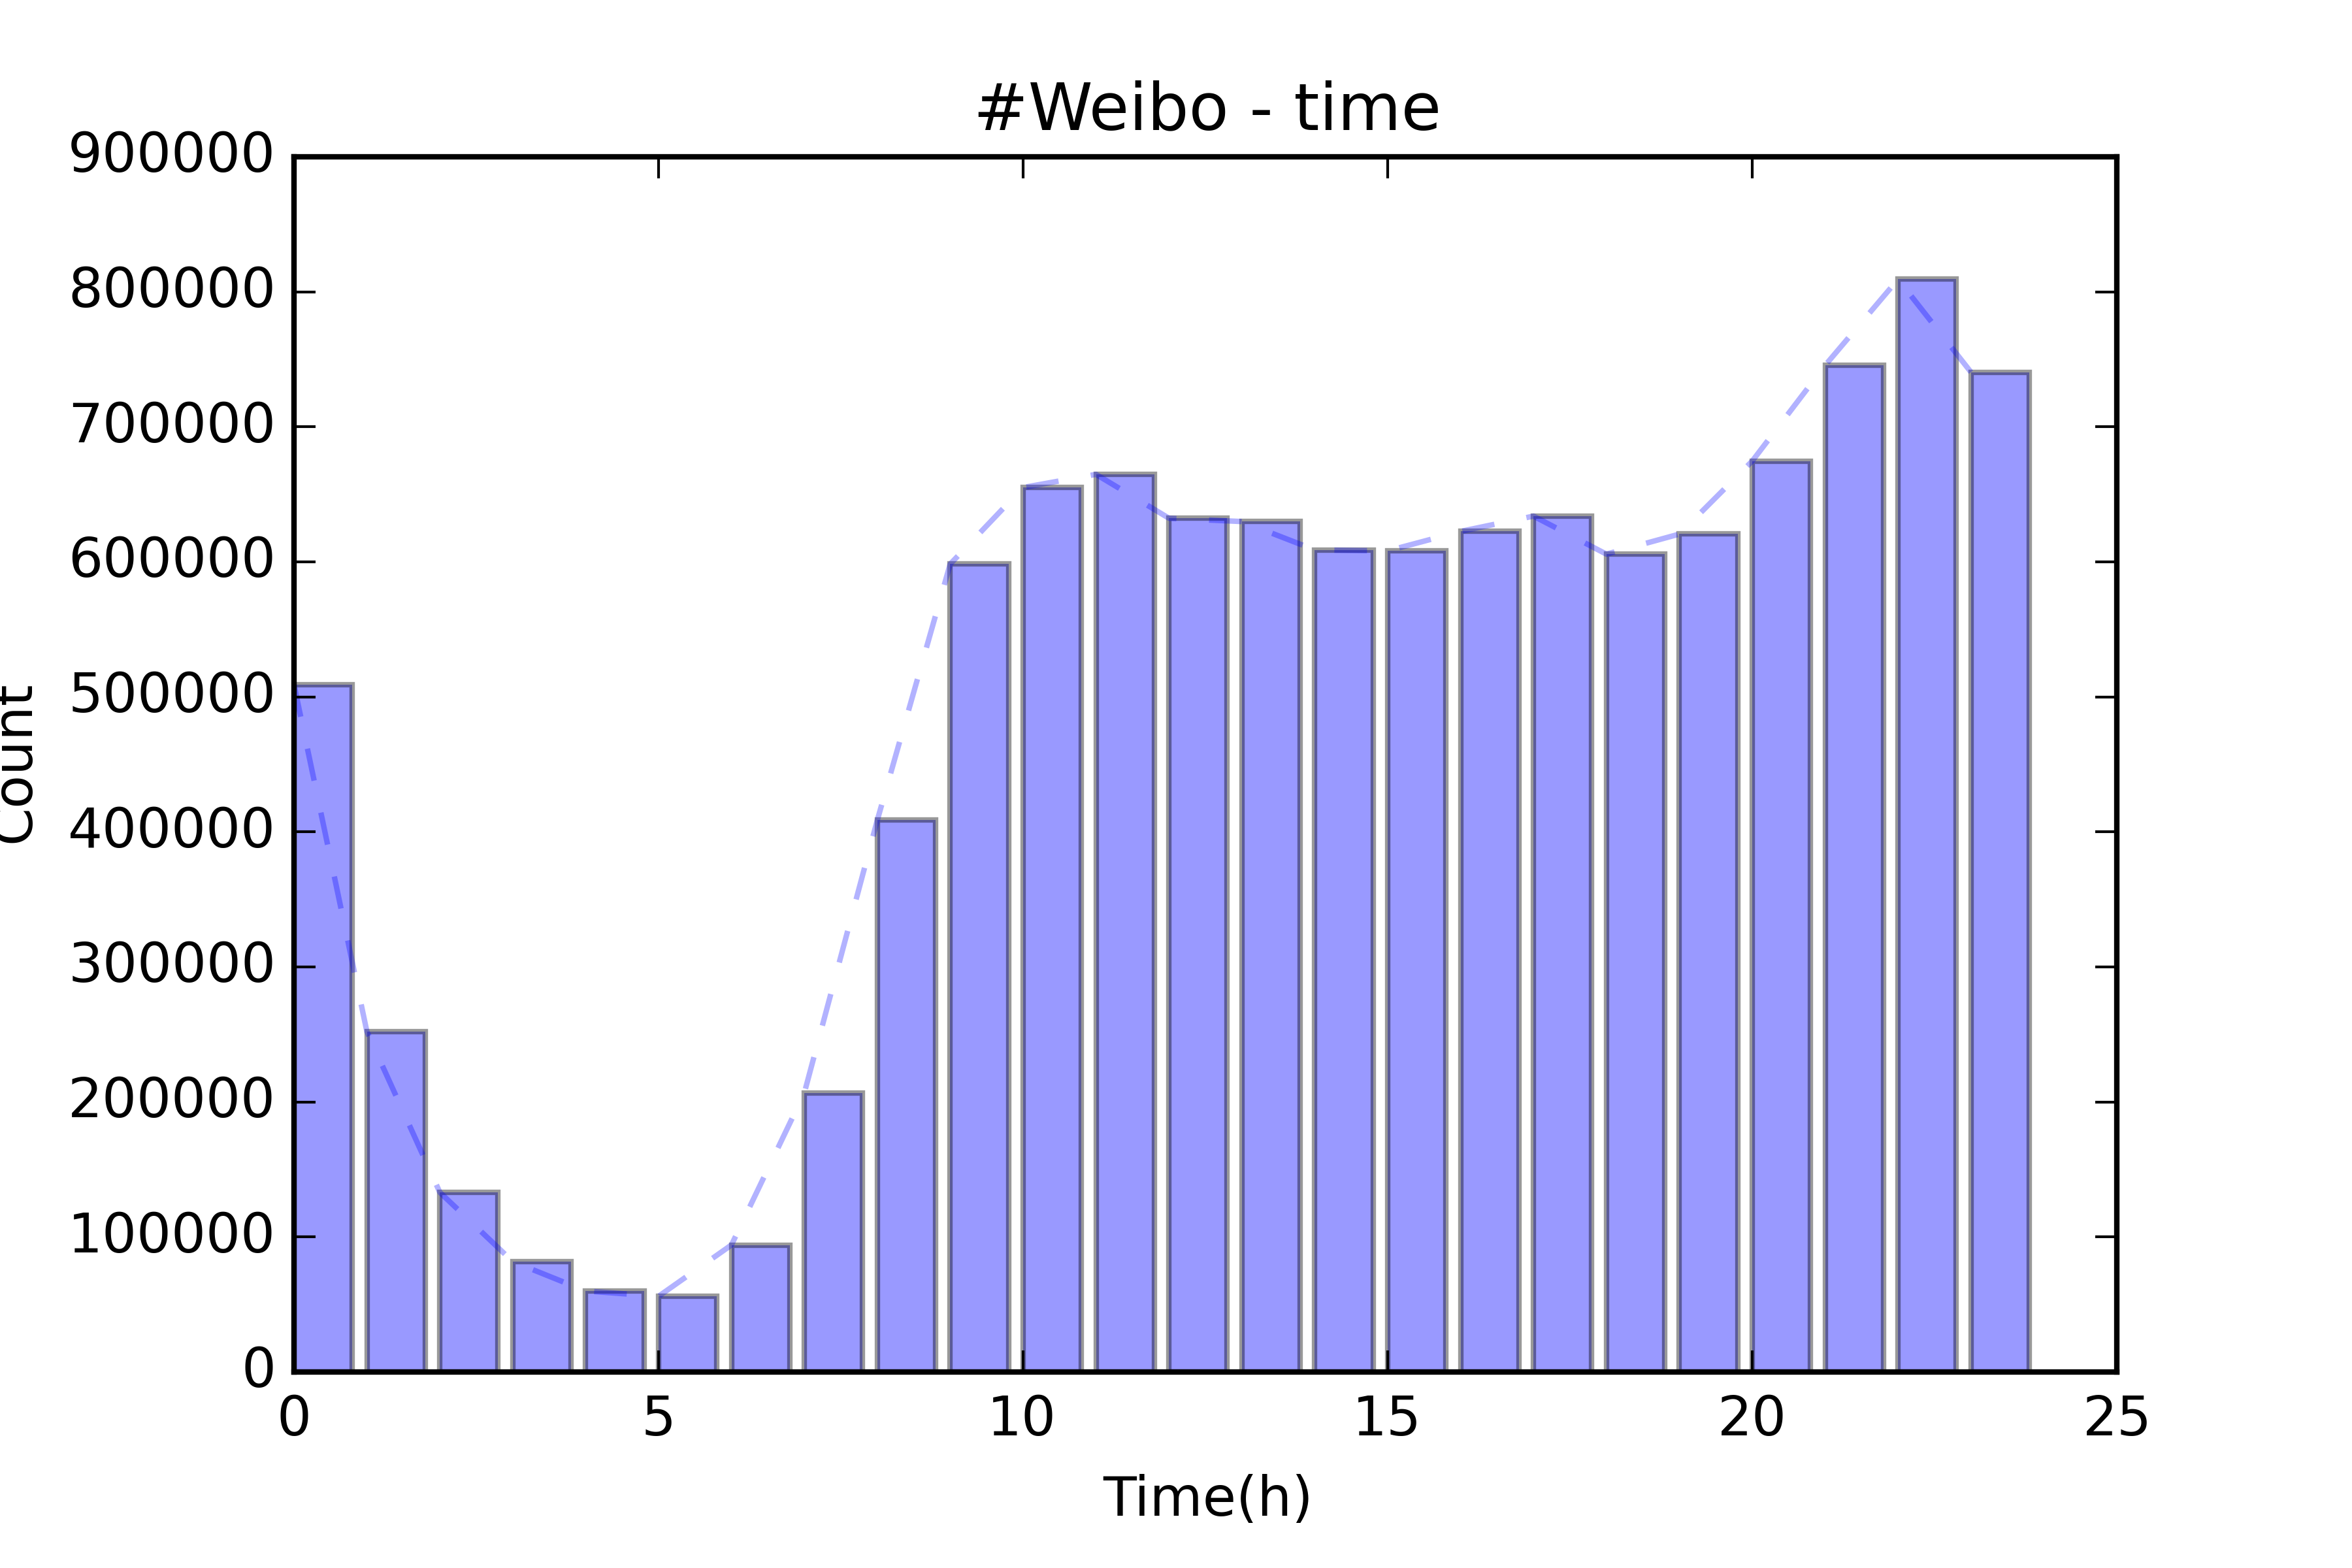
\includegraphics[width=0.8\linewidth]{../result/charts/weibo_time}
	\caption{微博量-时间}
	\label{fig:weibo_time}
\end{figure}

\subsection{微博情绪-时间}
\label{subsec:emotion_time}
在这一节中我们试图通过统计来揭示微博情绪随时间的变化情况。程序实现中, map 和 reduce 操作在\ref{subsec:weibo_time}节中已经介绍,这里补充说明 {\it(HH:MM, emotion)} 的 key-value pair 中 emotion 的计算方法。计算方法如下:
$$
emotion = 
\begin{cases}
1 & npos > 0~and~nneg = 0 \\
-1 & npos = 0~and~nneg > 0 \\
2 & nneg > 0~and~npos >= nneg \\
-2 & npos > 0~and~nneg > npos \\
0 & \text{otherwise}
\end{cases}
$$
公式中的 {\it npos, npeg} 为预处理后统计出来的两个数值,代表微博中包含的正负表情个数。 公式的结果中,1和-1代表这条微博具有明显的情绪倾向,0代表微博中不包含含有情绪的表情(或者表情不在数据集的情感词典中出现),2和-2代表这条微博的情绪有歧义,但更偏向积极或更偏向消极。

图\ref{fig:emotion_time_1}反映了有明确情绪的微博和总微博数量之间的关系。没有明确情绪的微博由上述 emotion 为 0和±2的微博组成。图\ref{fig:emotion_time_2}反映了积极微博和消极微博数量上的关系,可以明显的看出,情感积极的微博总是占据大多数的。为了更好的体现微博整体情感的变化趋势,我们使用 {\it PN ratio} 来衡量整个微博的情感。
$$PN~ratio = \frac{\text{\#positive weibo}}{\text{\#negative weibo}}$$
图\ref{fig:emotion_time_3}反映了 {\it PN ratio} 与时间的关系。有意思的是,整体的图形与微博量-时间的图形非常相似,这也就意味着,在深夜的时候,消极微博占的比重更大。全天来看,4时开始整体开始往积极方向发展,而到了15时之后,则开始往消极方向发展。

\begin{figure}
	\centering
	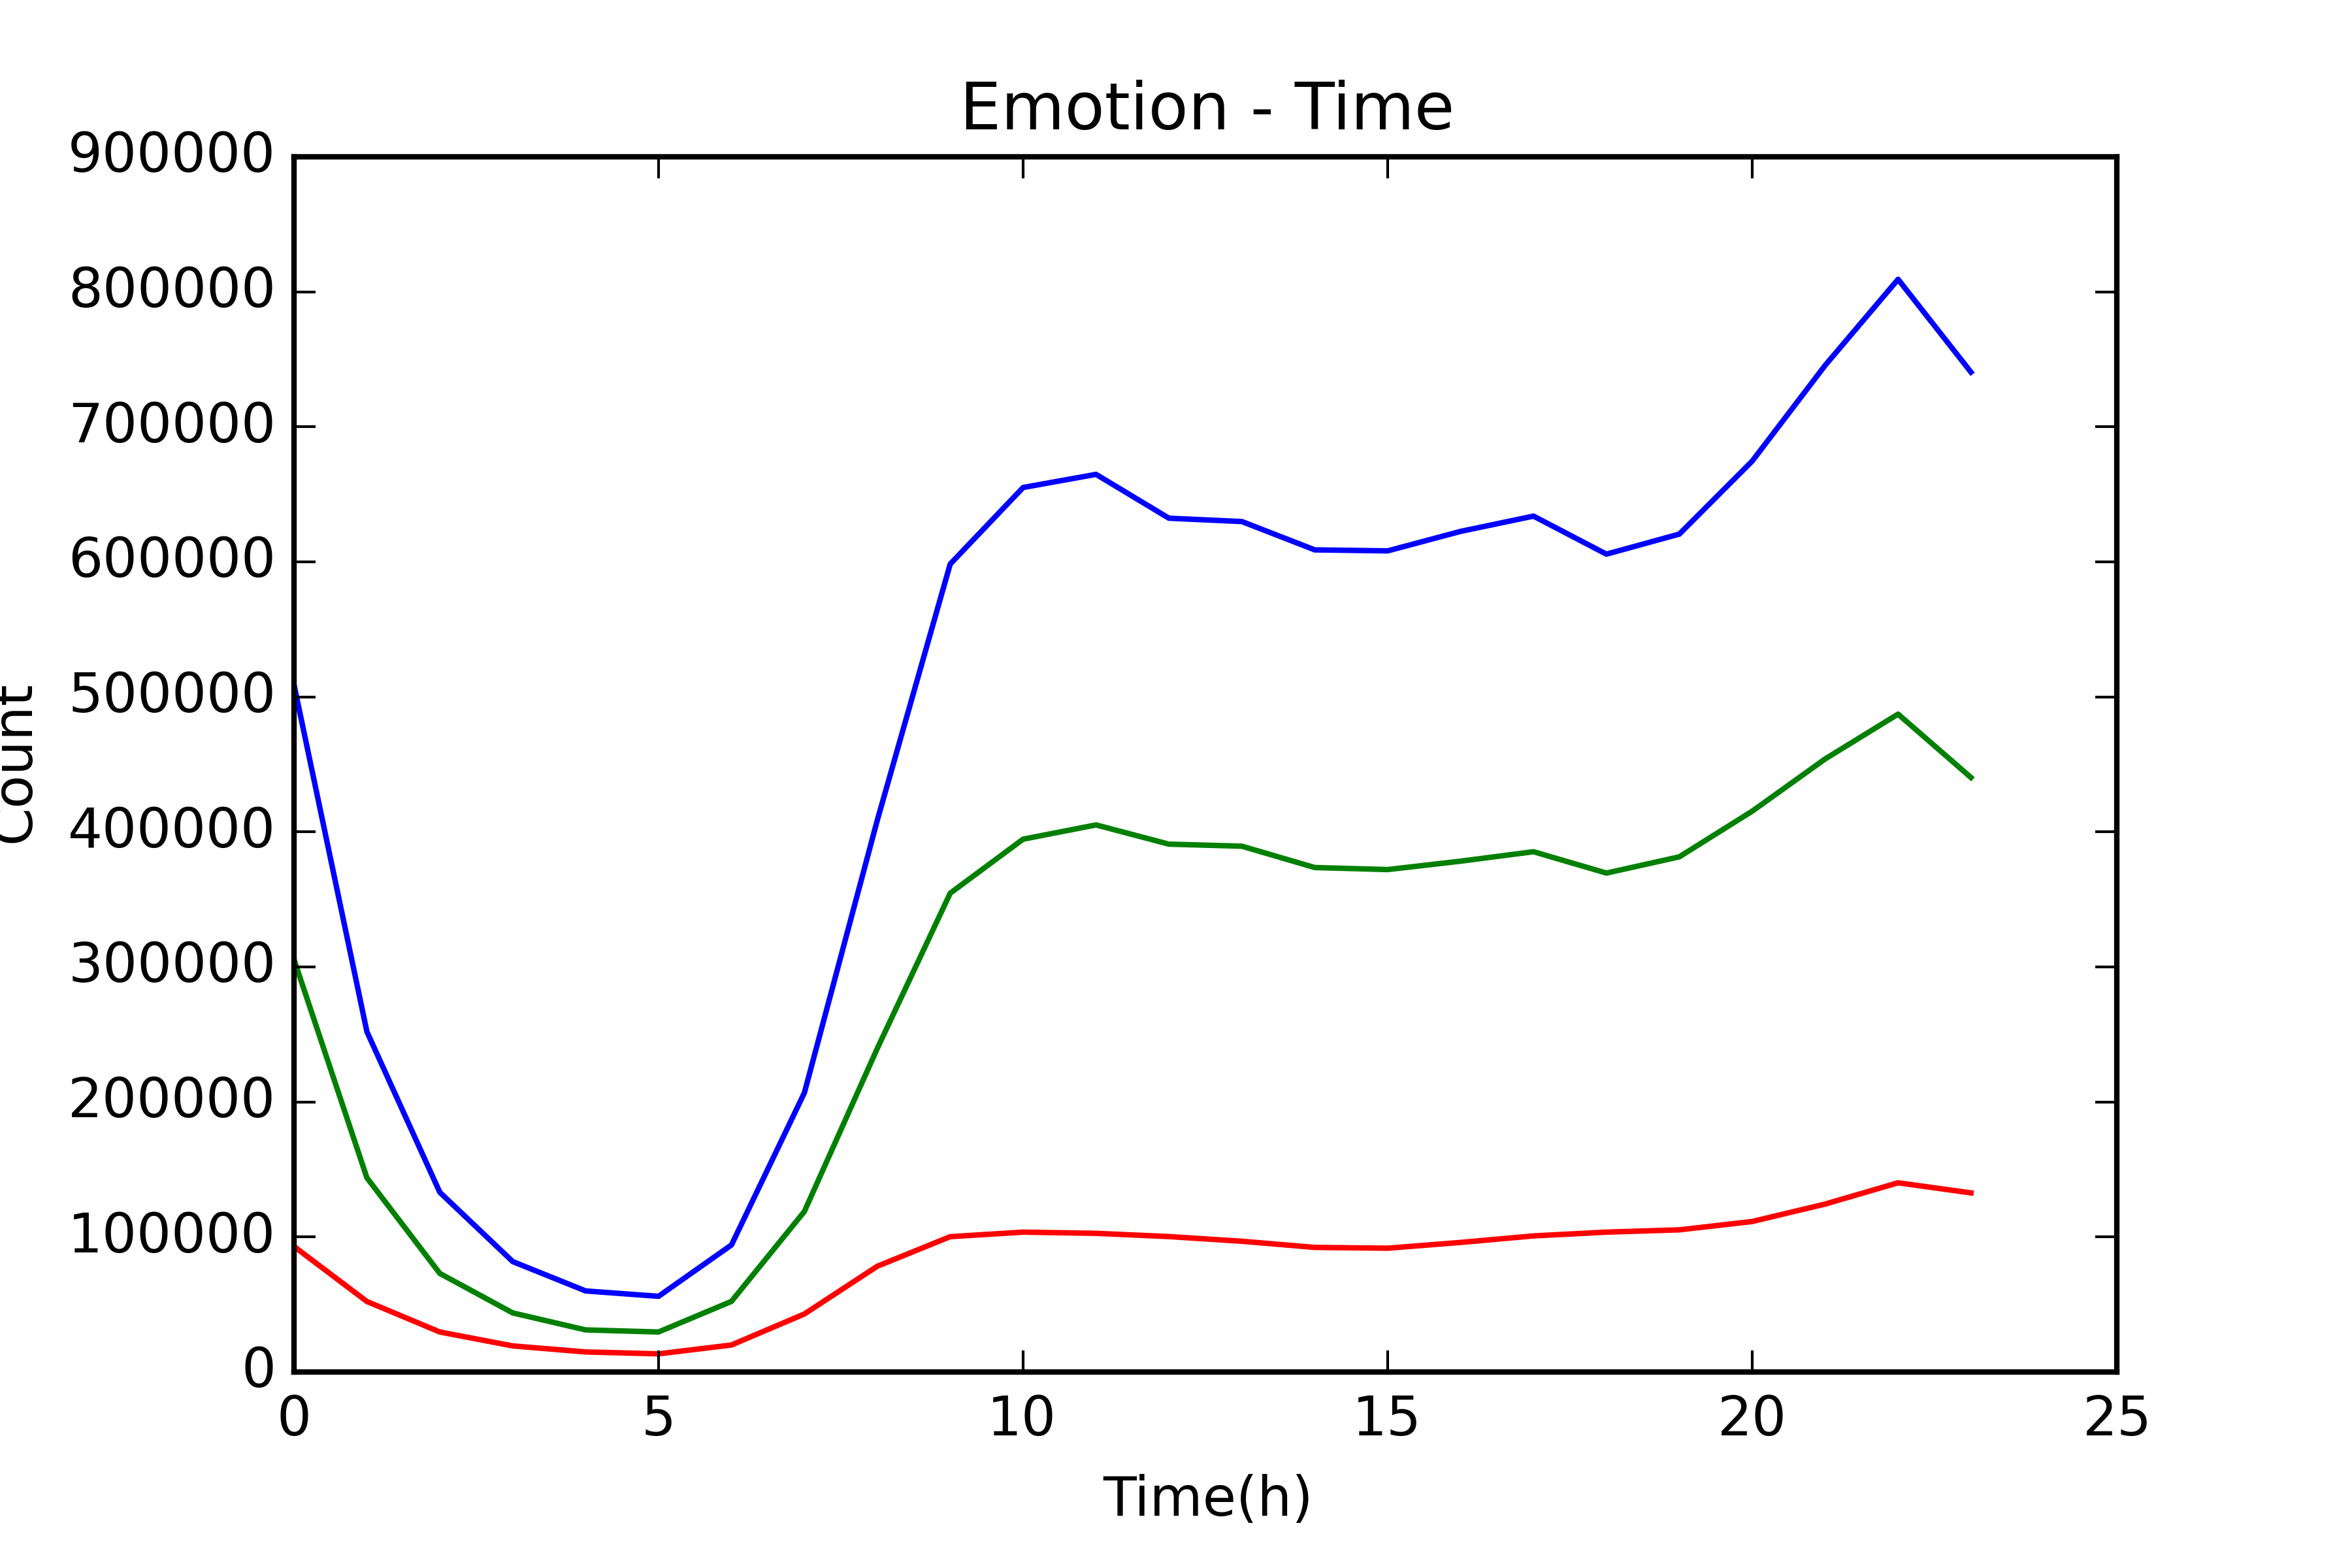
\includegraphics[width=0.8\linewidth]{../result/charts/emotion_time_1}
	\caption{有明确微博和总微博数量的关系。图中绿色线表示所有微博量,蓝色为积极情绪,红色为消极情绪。}
	\label{fig:emotion_time_1}
\end{figure}
\begin{figure}
	\centering
	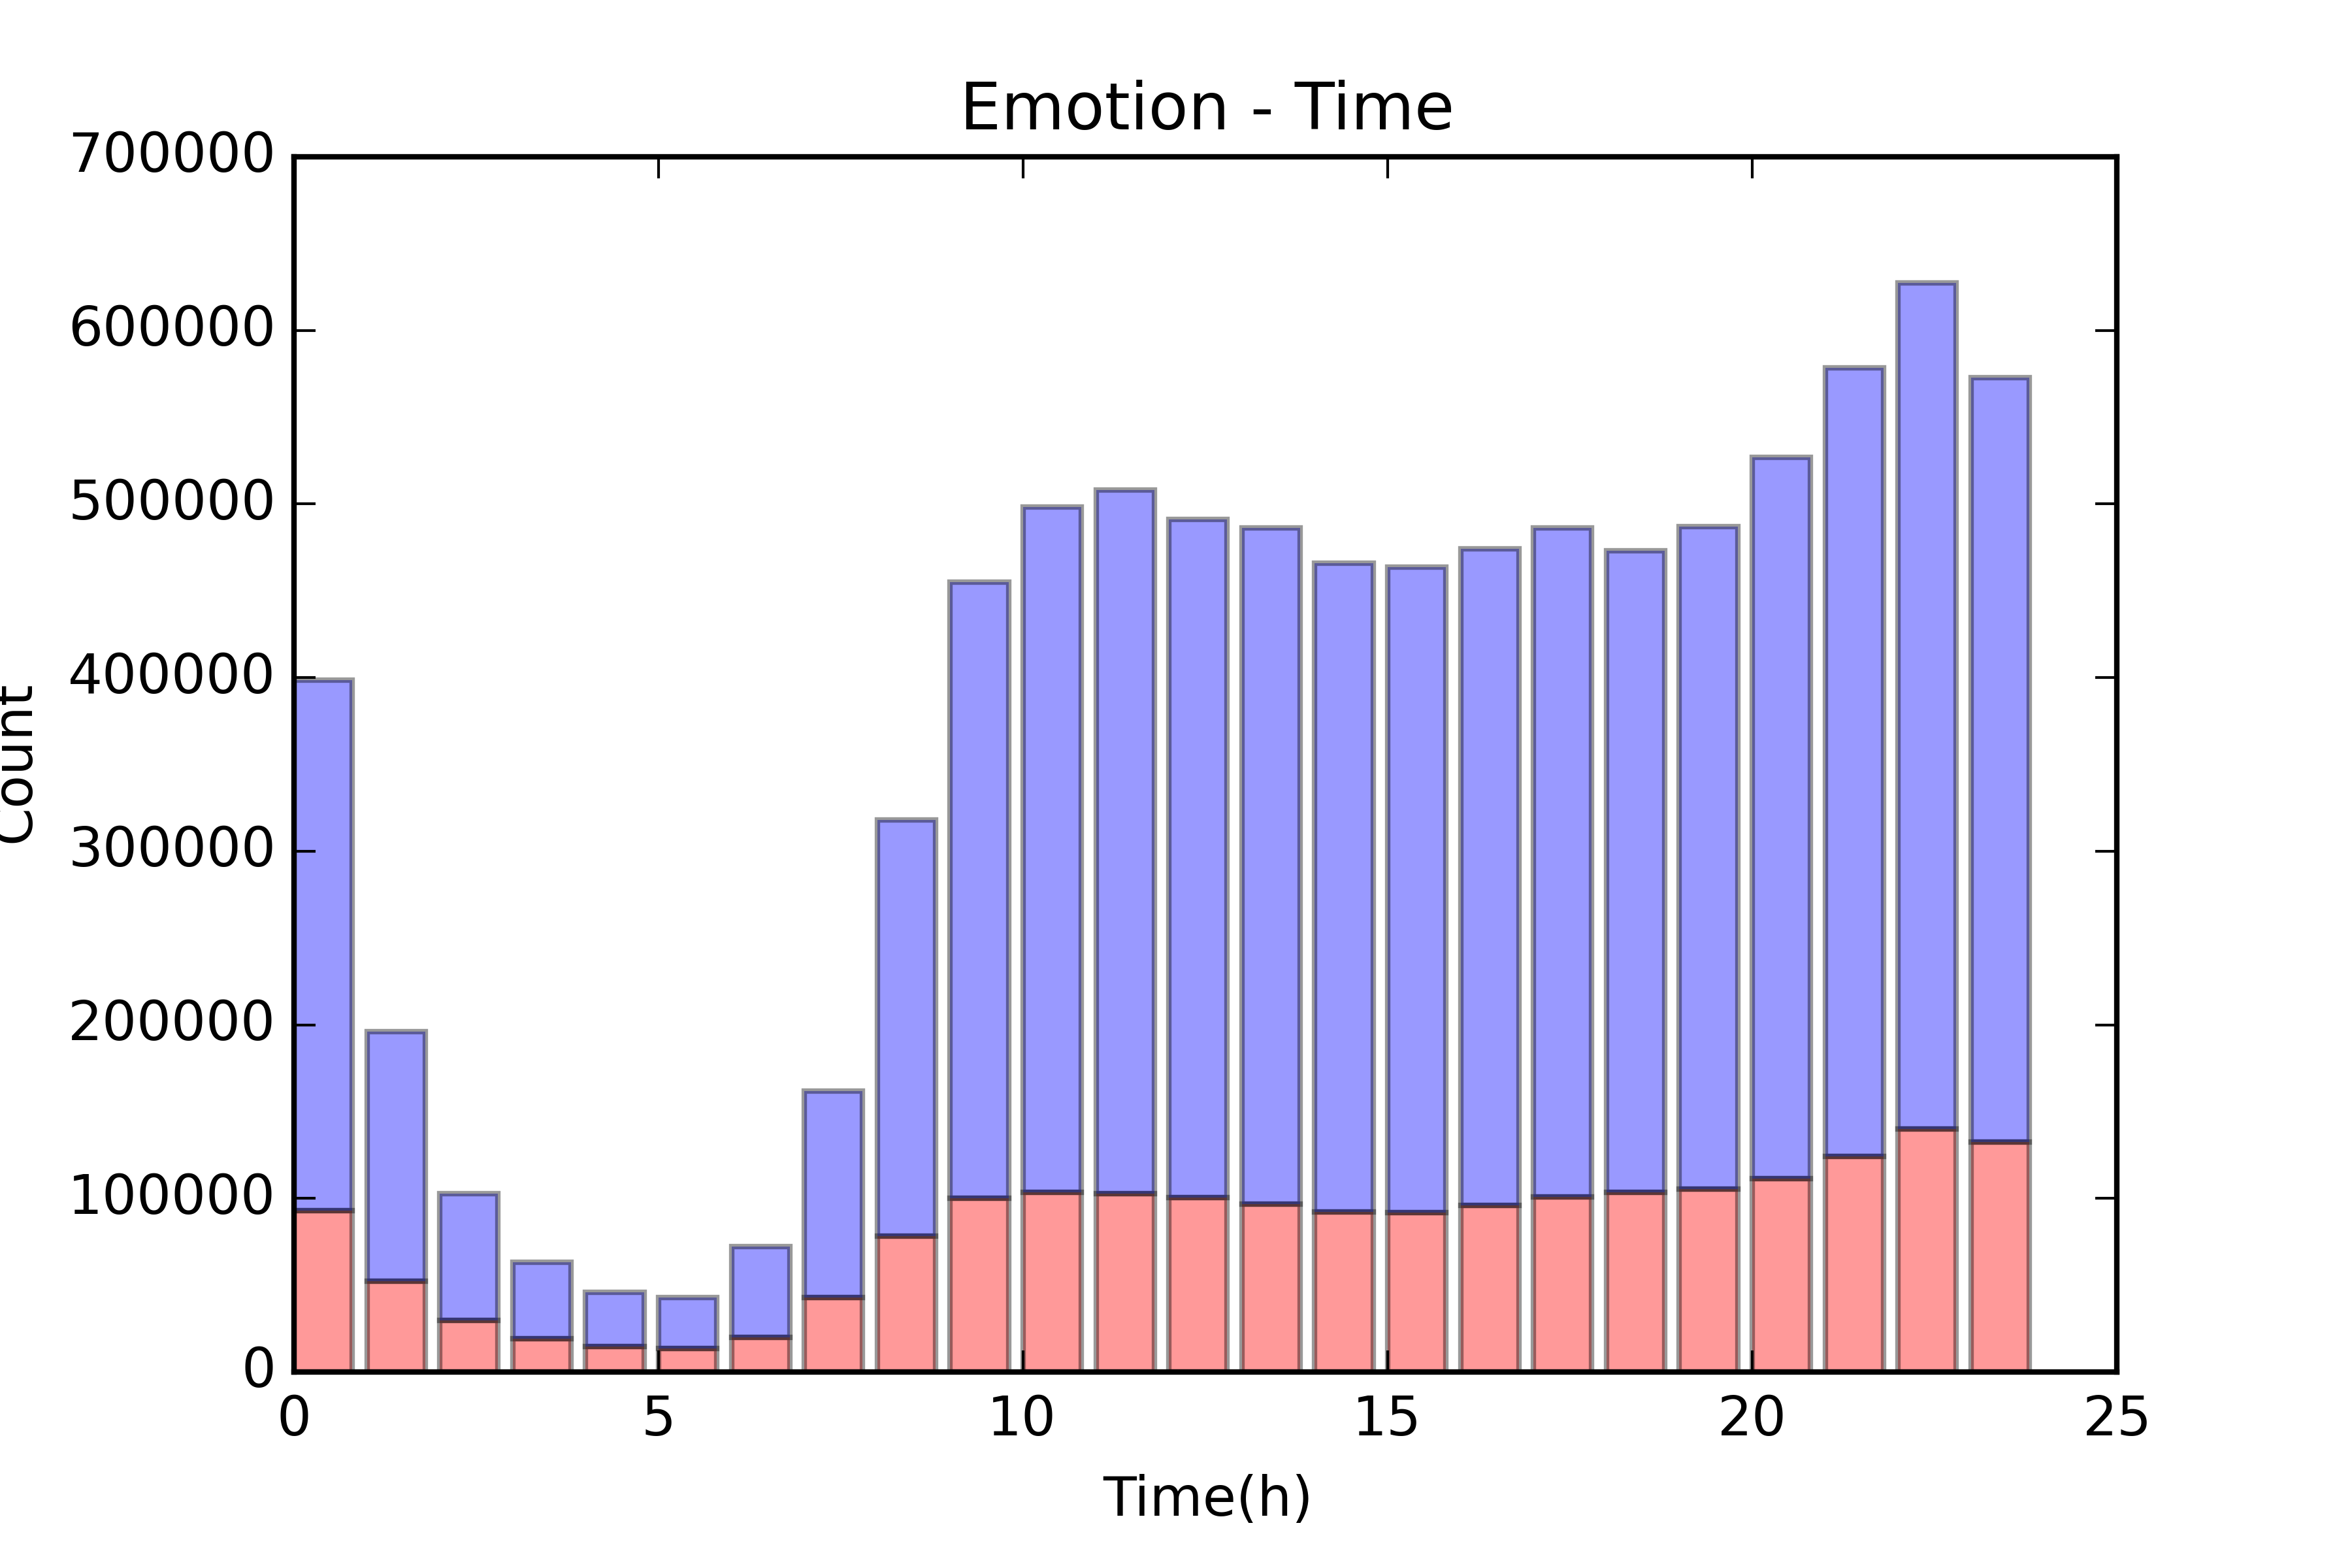
\includegraphics[width=0.8\linewidth]{../result/charts/emotion_time_2}
	\caption{微博情绪-时间(不包括没有明确情绪的微博)。图中蓝色代表积极情绪,红色代表消极情绪,蓝色柱堆叠于红色柱上方。}
	\label{fig:emotion_time_2}
\end{figure}
\begin{figure}
	\centering
	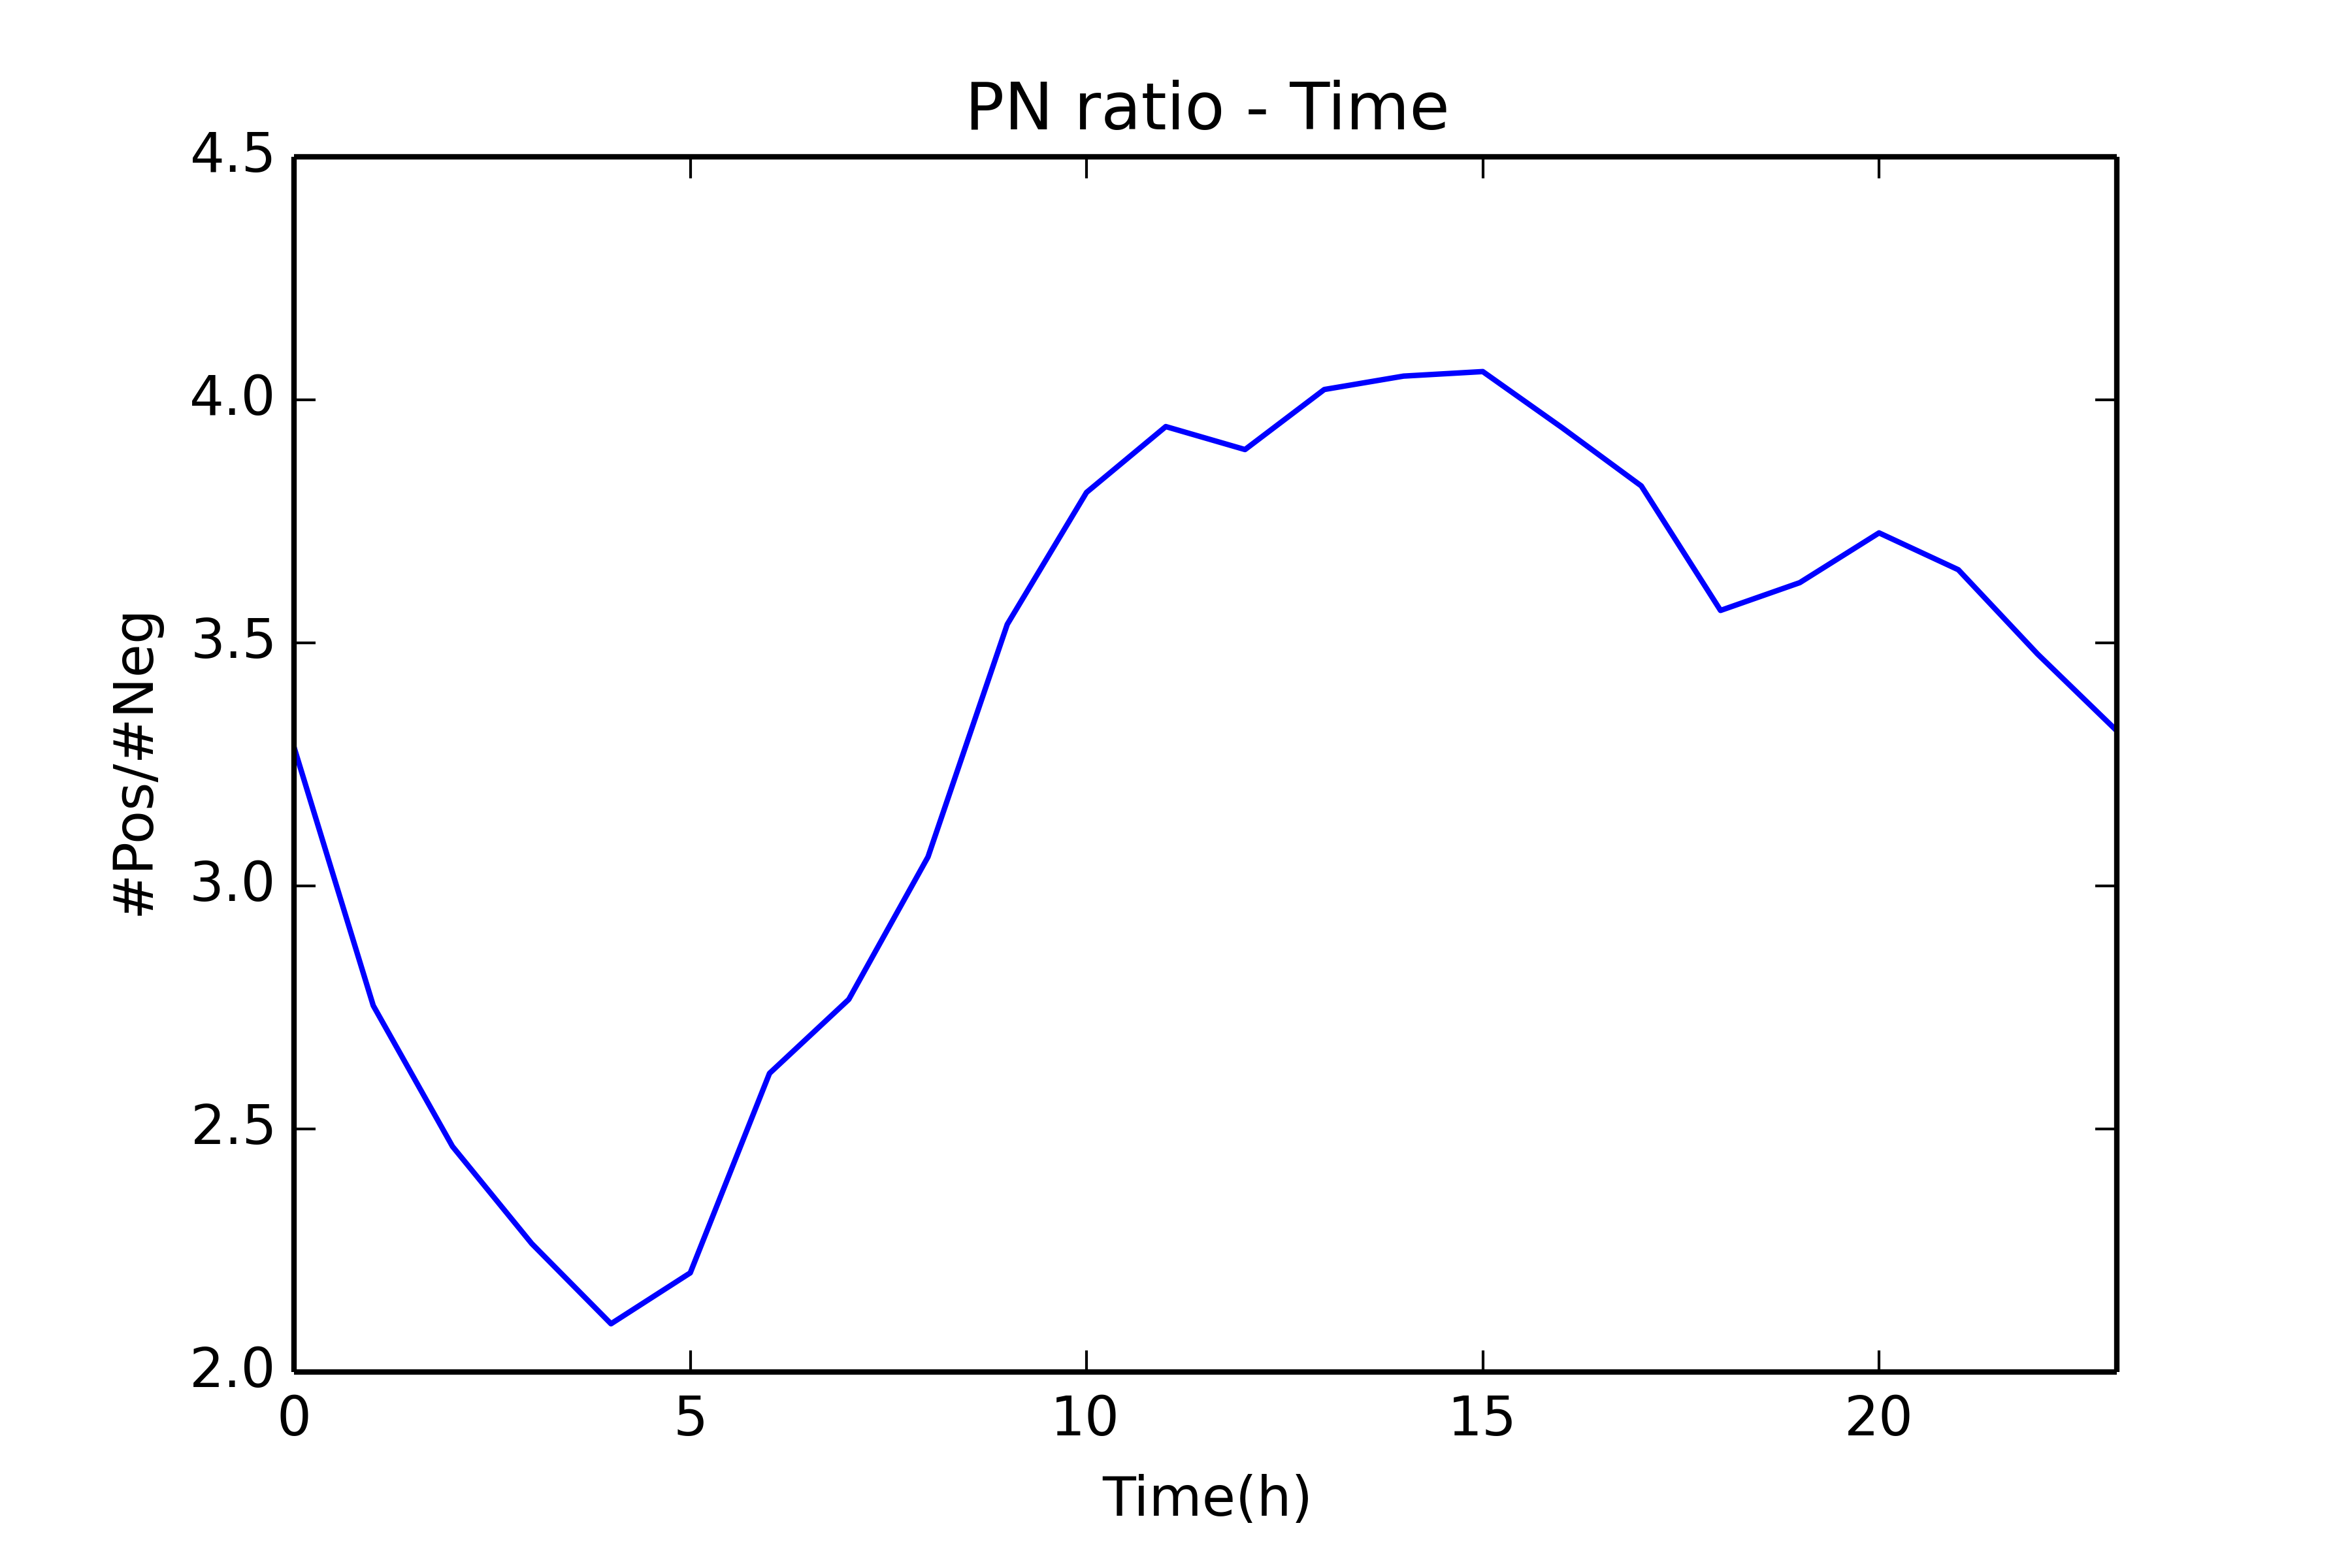
\includegraphics[width=0.8\linewidth]{../result/charts/emotion_time_3}
	\caption{积极与消极微博比例和时间的关系。}
	\label{fig:emotion_time_3}
\end{figure}

\subsection{微博情绪-日期}
这一小节我们分析每日微博情绪(使用 {\it PN ratio} 衡量)波动,并以此检验衡量标准是否有效。从\cite{bollen2011twitter}中作者的实验来看,好的衡量标准应该能够准确的反映重大公众事件的发生。因此我们在实验之前,预期 {\it PN ratio} 在春节等节日应该达到最大,在5·12等纪念日时达到低谷。

实验结果符合我们的预期, {\it PN ratio} 能够如实体现重大公众事件发生后大众心理的变化。积极情绪中:2012年01月01日,元旦,微博情绪达到了全年最高峰, {\it PN ratio} 为5.87。2012年01月22日,除夕,{\it PN ratio} 达到了另一个极大值5.76。随后的大年初一,该值仍维持较高的水平,达到5.51。到了2012年01月28日,春节7天假期结束,上班族不得不重返工作岗位,微博相应的出现了较多的消极情绪,这一天 {\it PN ratio} 为2.96。全年还有两个明显的峰值,一个是在2012年02月14日的情人节,另一个则是在2012年06月01日的六一儿童节。

消极情绪方面:2012年05月12日,汶川大地震四周年,微博上包括名人、机构在内的众多网友纷纷发微博表示悼念, {\it PN ratio} 为2.29。此外,2012年07月22日和2012年07月23日两天达到了全年的最低谷, {\it PN ratio} 分别为2.09和2.19。经过采样分析,主要与两件事情有关,一是2012年07月22日重创北京的大暴雨,二是2011年7月23日发生的甬台温铁路列车追尾事故。两件事情的叠加,使得微博上出现了更多悼念和问责的声音,最终把情绪拉向了全年的最低谷。初次之外,2012年01月28日还出现了一次低谷,{\it PN ratio} 为2.96,经过分析,与惠特尼·休斯顿去世有关。通过数据还可以类似的找出其于公众事件的关联,在此不再赘述。

\begin{figure}
	\centering
	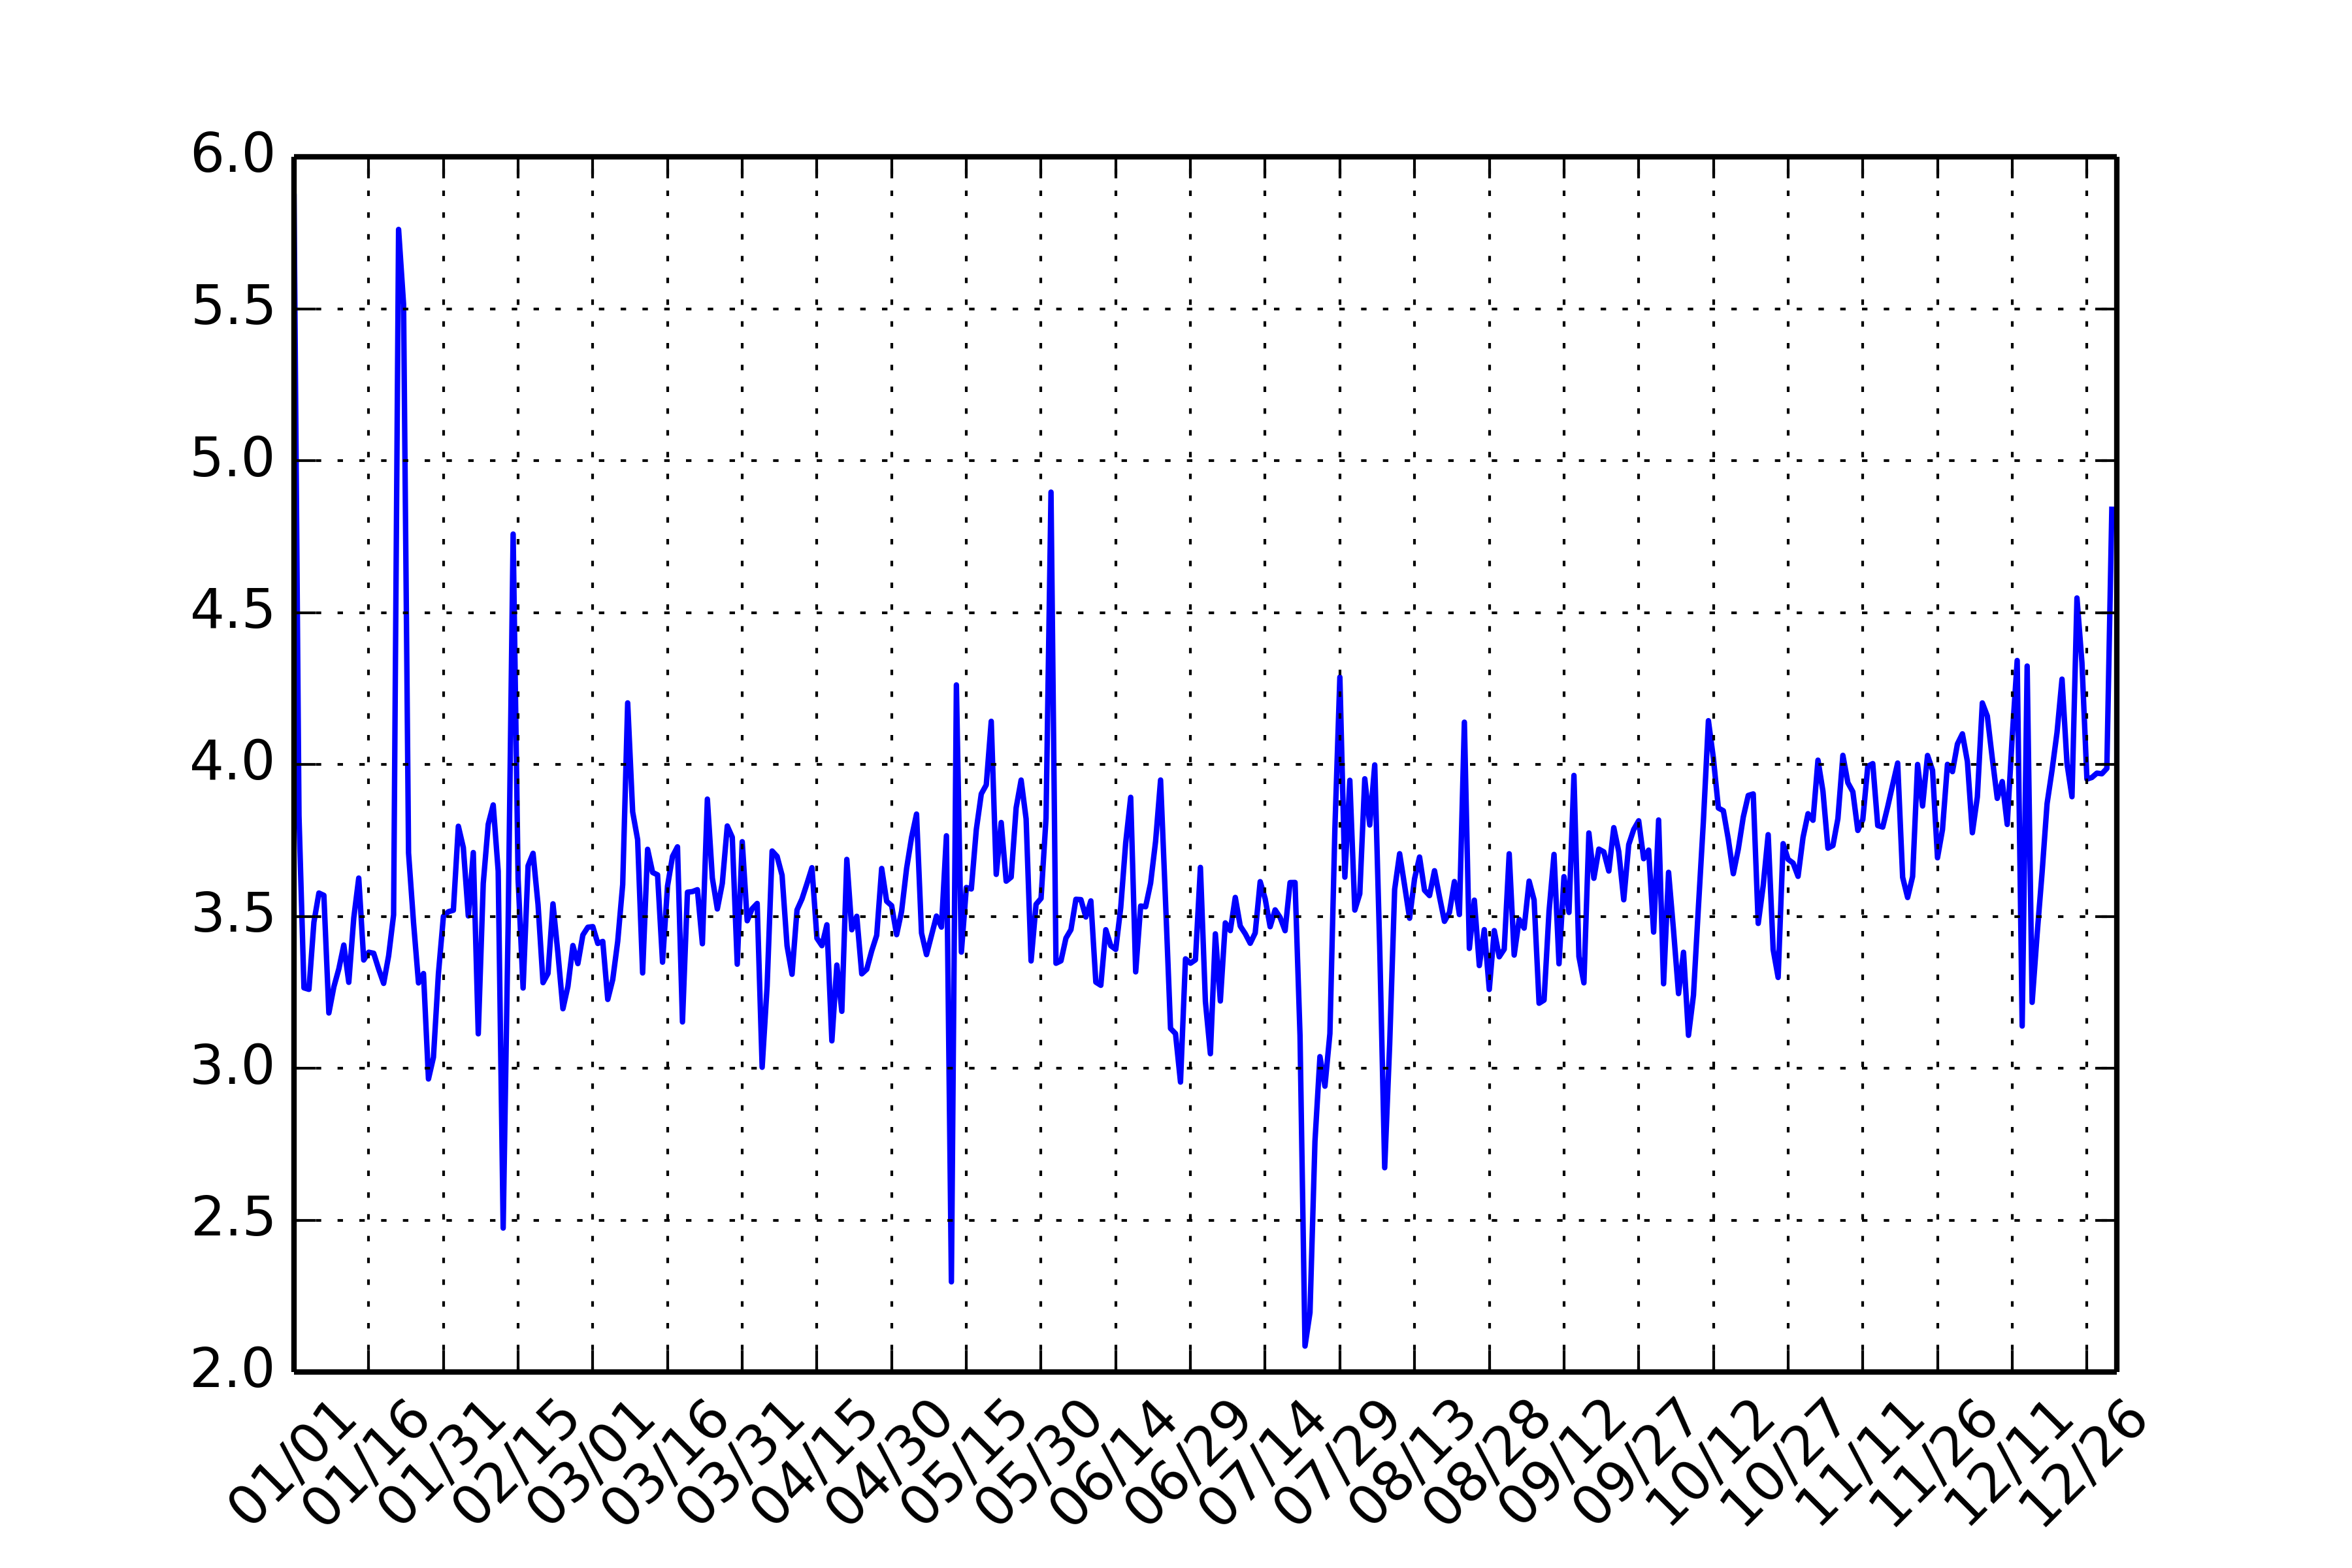
\includegraphics[width=0.8\linewidth]{../result/charts/emotion_day}
	\caption{2012年日微博情绪波动。}
	\label{fig:emotion_day}
\end{figure}

\subsection{微博情绪-性别}
这一小节分析微博情绪在男女之中是否有所差别。从数据中看,积极微博的占比在男女性中不相上下,而女性的消极微博占比要多出约2个百分点。

\begin{figure}
	\centering
	\begin{subfigure}[b]{0.45\linewidth}
		\centering
		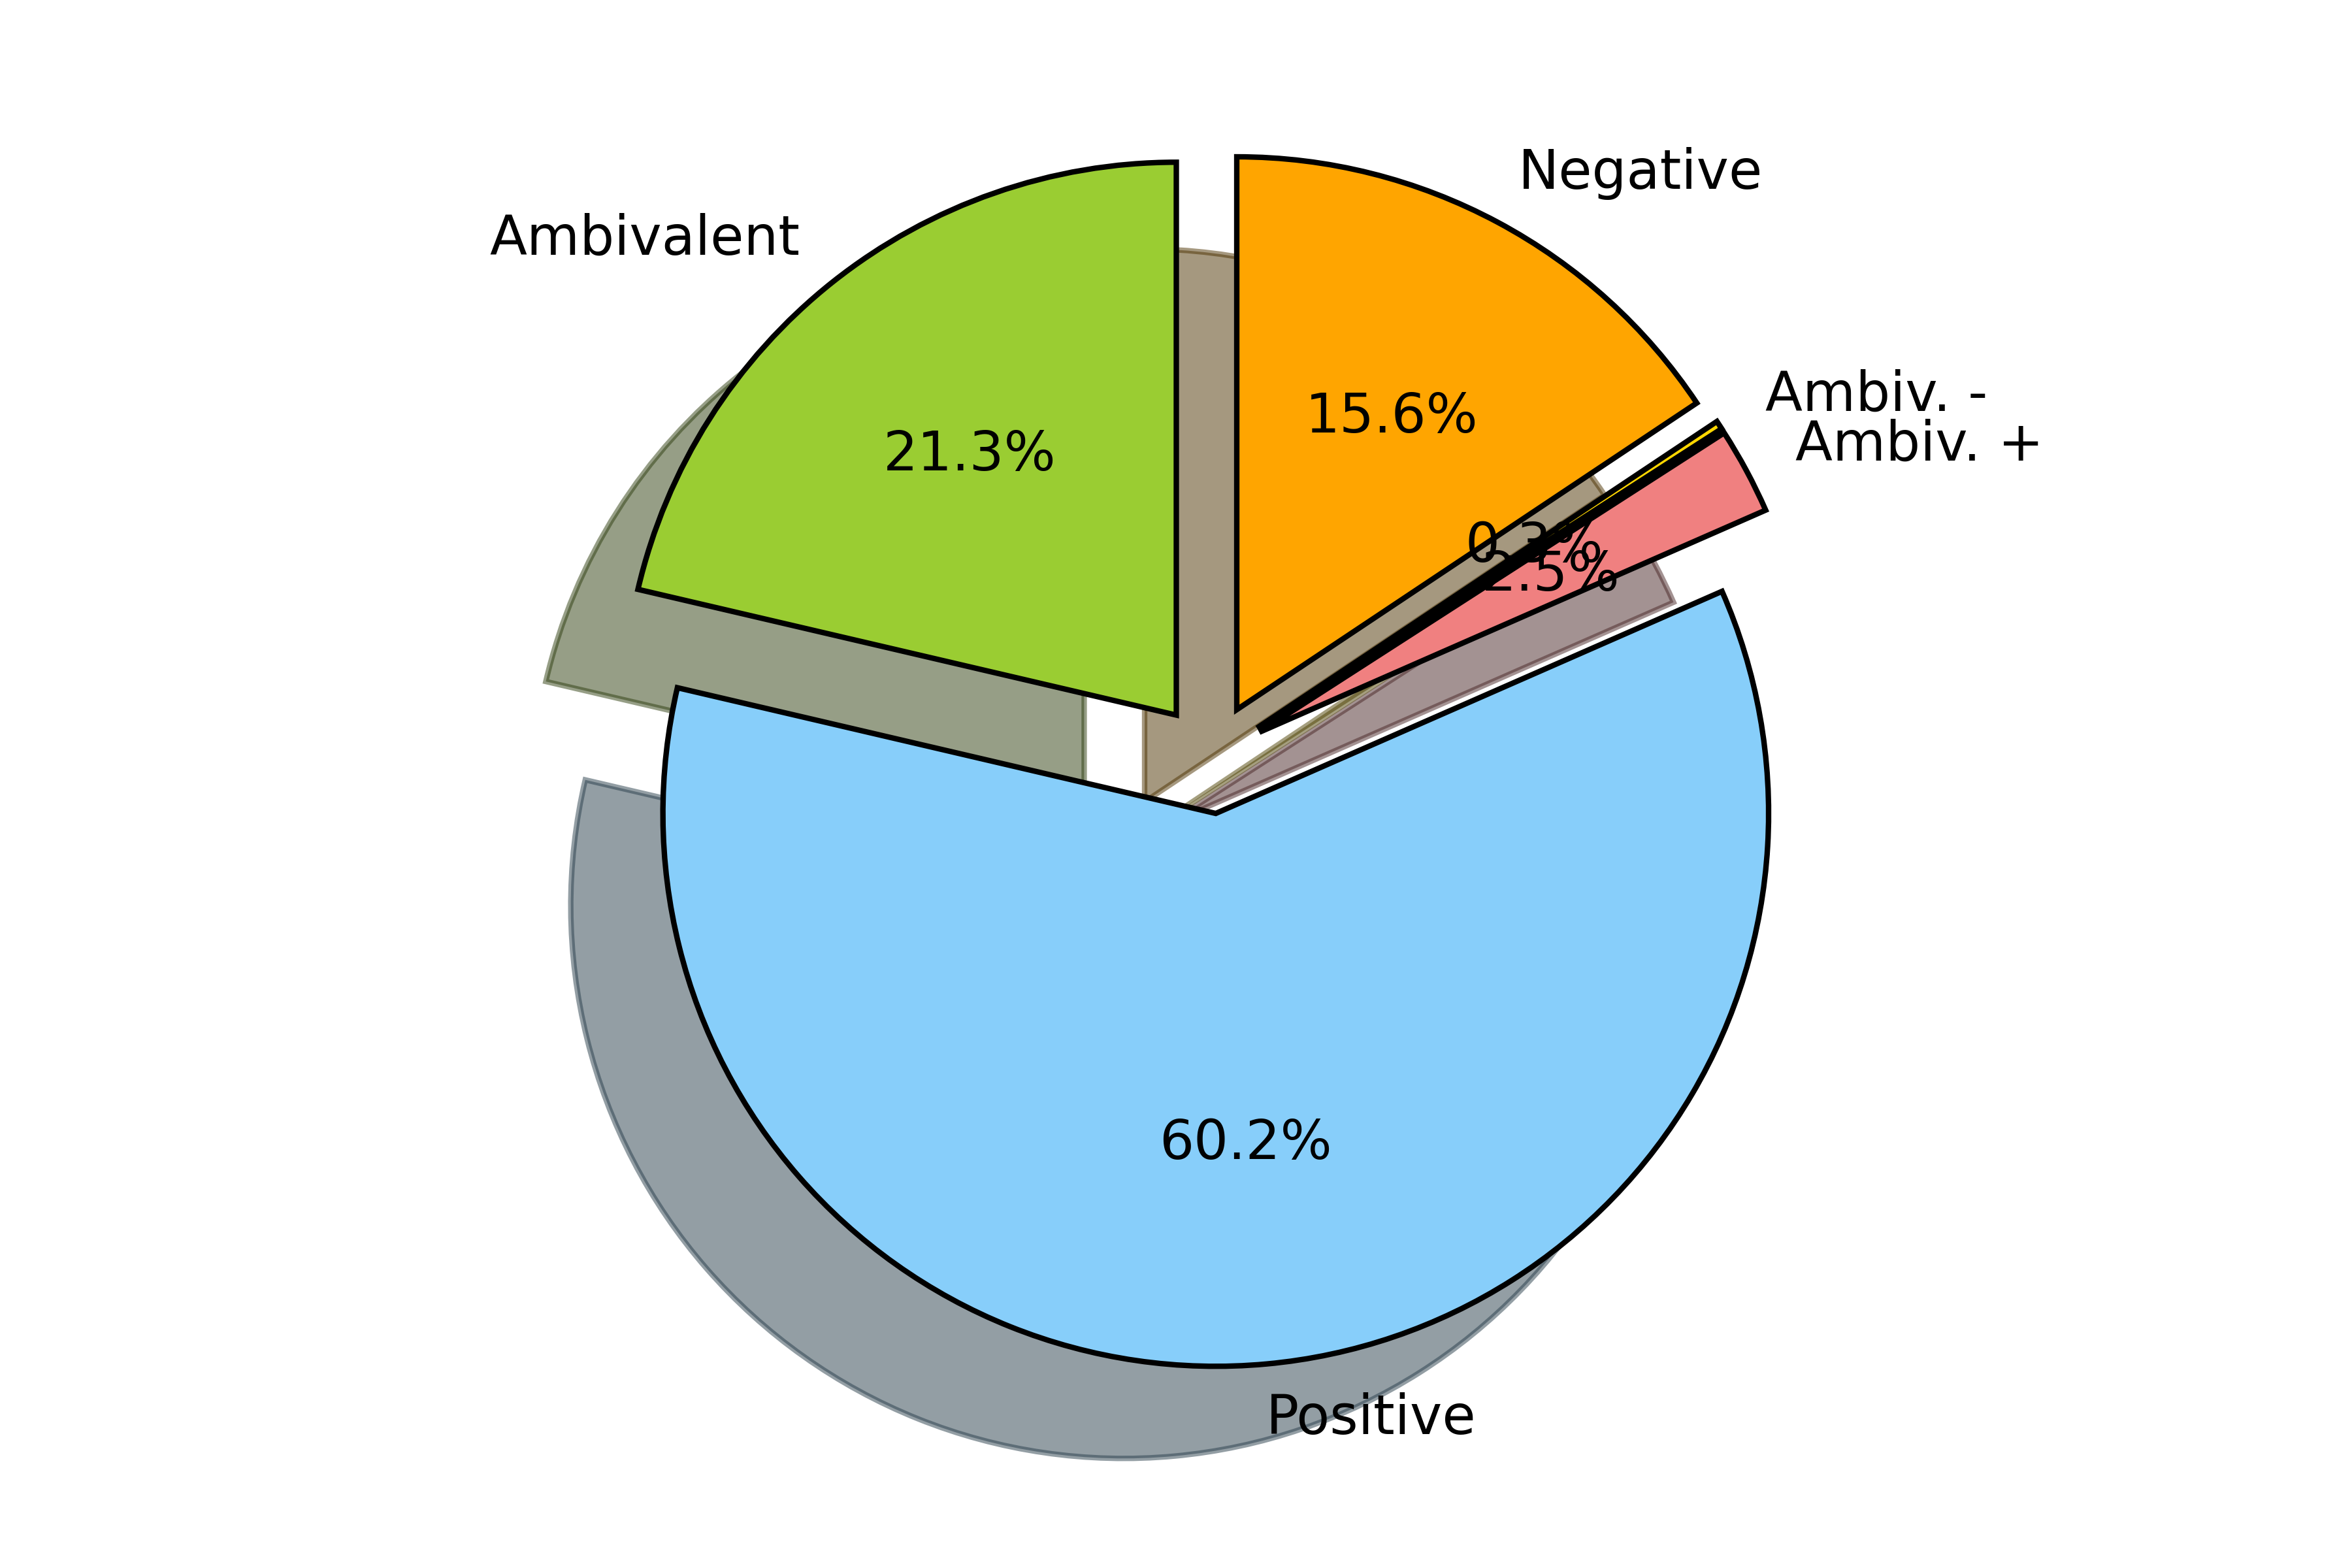
\includegraphics[trim = 1.5cm 0 1.5cm 0, clip = true, width=\textwidth]{../result/charts/emotion_gender_m}
		\caption{男性}
	\end{subfigure}
	\begin{subfigure}[b]{0.45\linewidth}
		\centering
		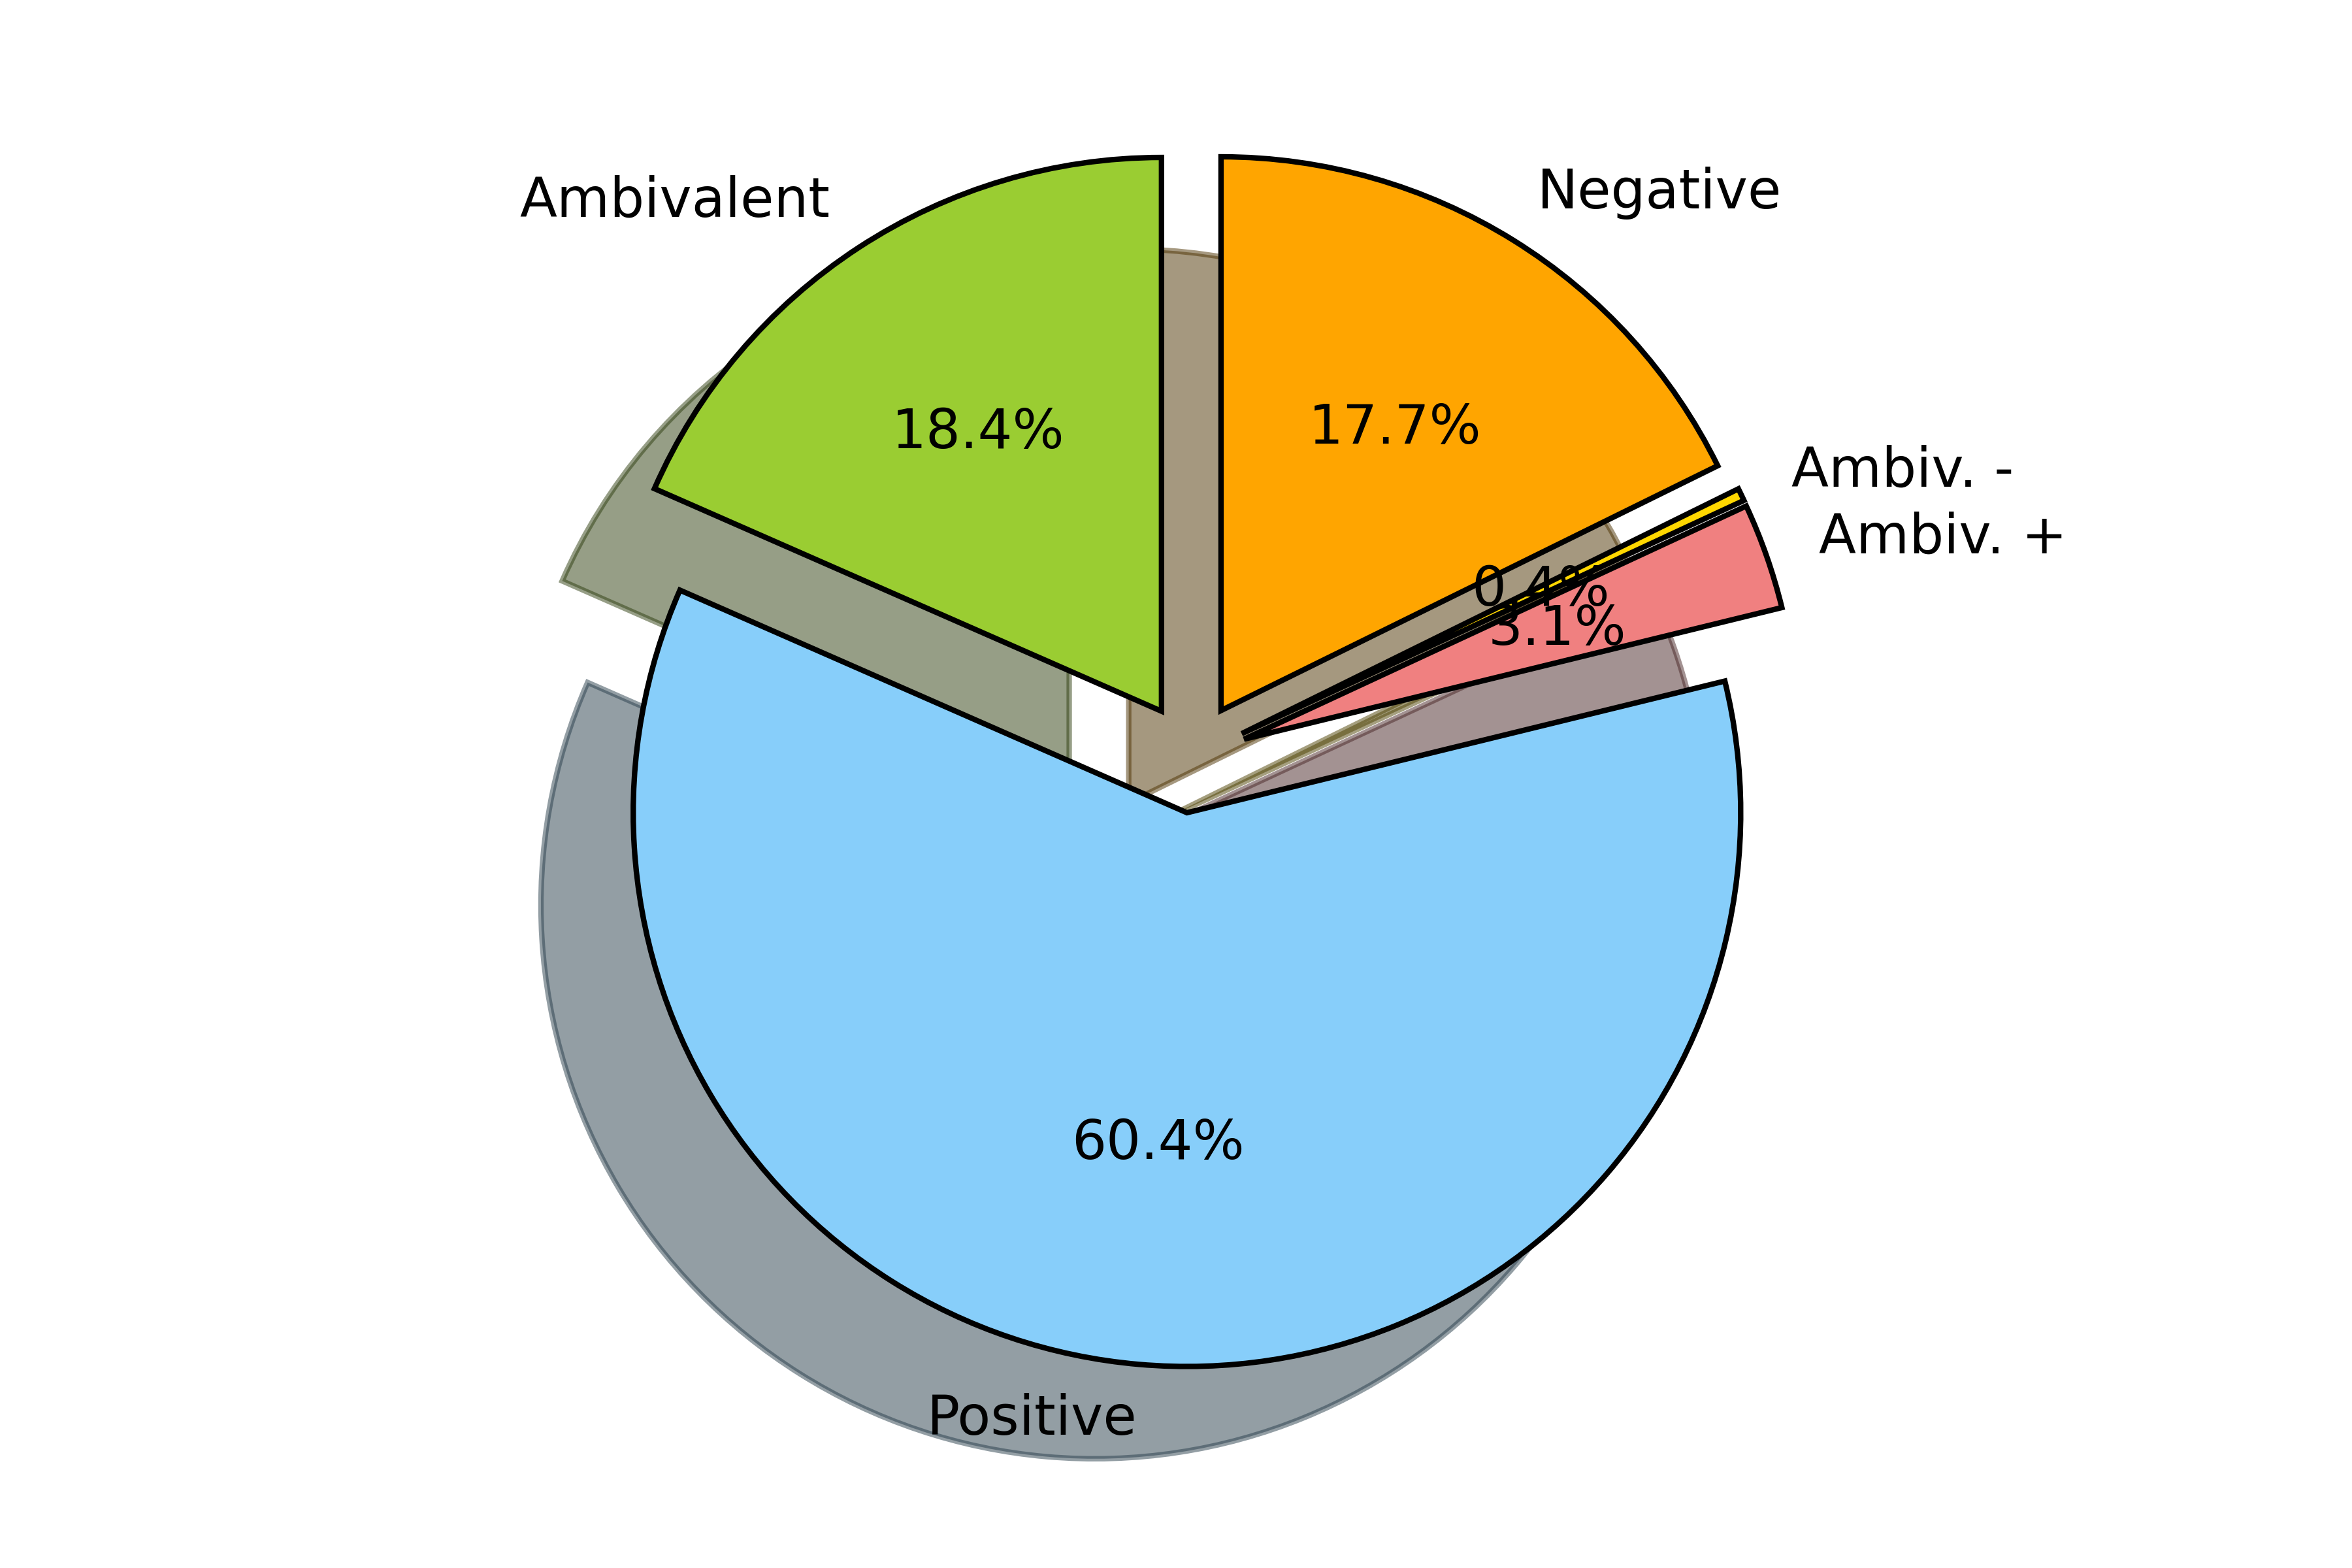
\includegraphics[trim = 1.5cm 0 1.5cm 0, clip = true, width=\textwidth]{../result/charts/emotion_gender_f}
		\caption{女性}
	\end{subfigure}
	\caption{各种微博情绪在不同性别人群里的分布。(图中蓝色代表积极情绪的微博,绿色代表无情绪,橙色代表消极情绪,剩余两类为有歧义的微博)}
	\label{fig:emotion_gender}
\end{figure}

\subsection{微博情绪-身份}
从图\ref{fig:emotion_identification}中蓝色部分(积极的微博)可以看出,最积极的是学校的微博,其次是企业和名人所发。原来预计政府应该在这一项中有最高的比重,但是可以看到,由于政府的微博有很大一部分被划分为无表情一类,推测可能的原因是政府使用的表情更偏向那些没有明显感情色彩的表情。另一方面,从消极占比来看,政府的消极微博占比则相较总体情况要少了很多,由此可以判断政府的微博还是比大部分的用户要更加积极的。除了政府,学校、名人、企业和媒体相对来说负面情绪要少一些,而负面情绪在微博会员这一类别中表现的更强烈。

\begin{figure}
	\centering
	\begin{subfigure}[b]{0.3\linewidth}
		\centering
		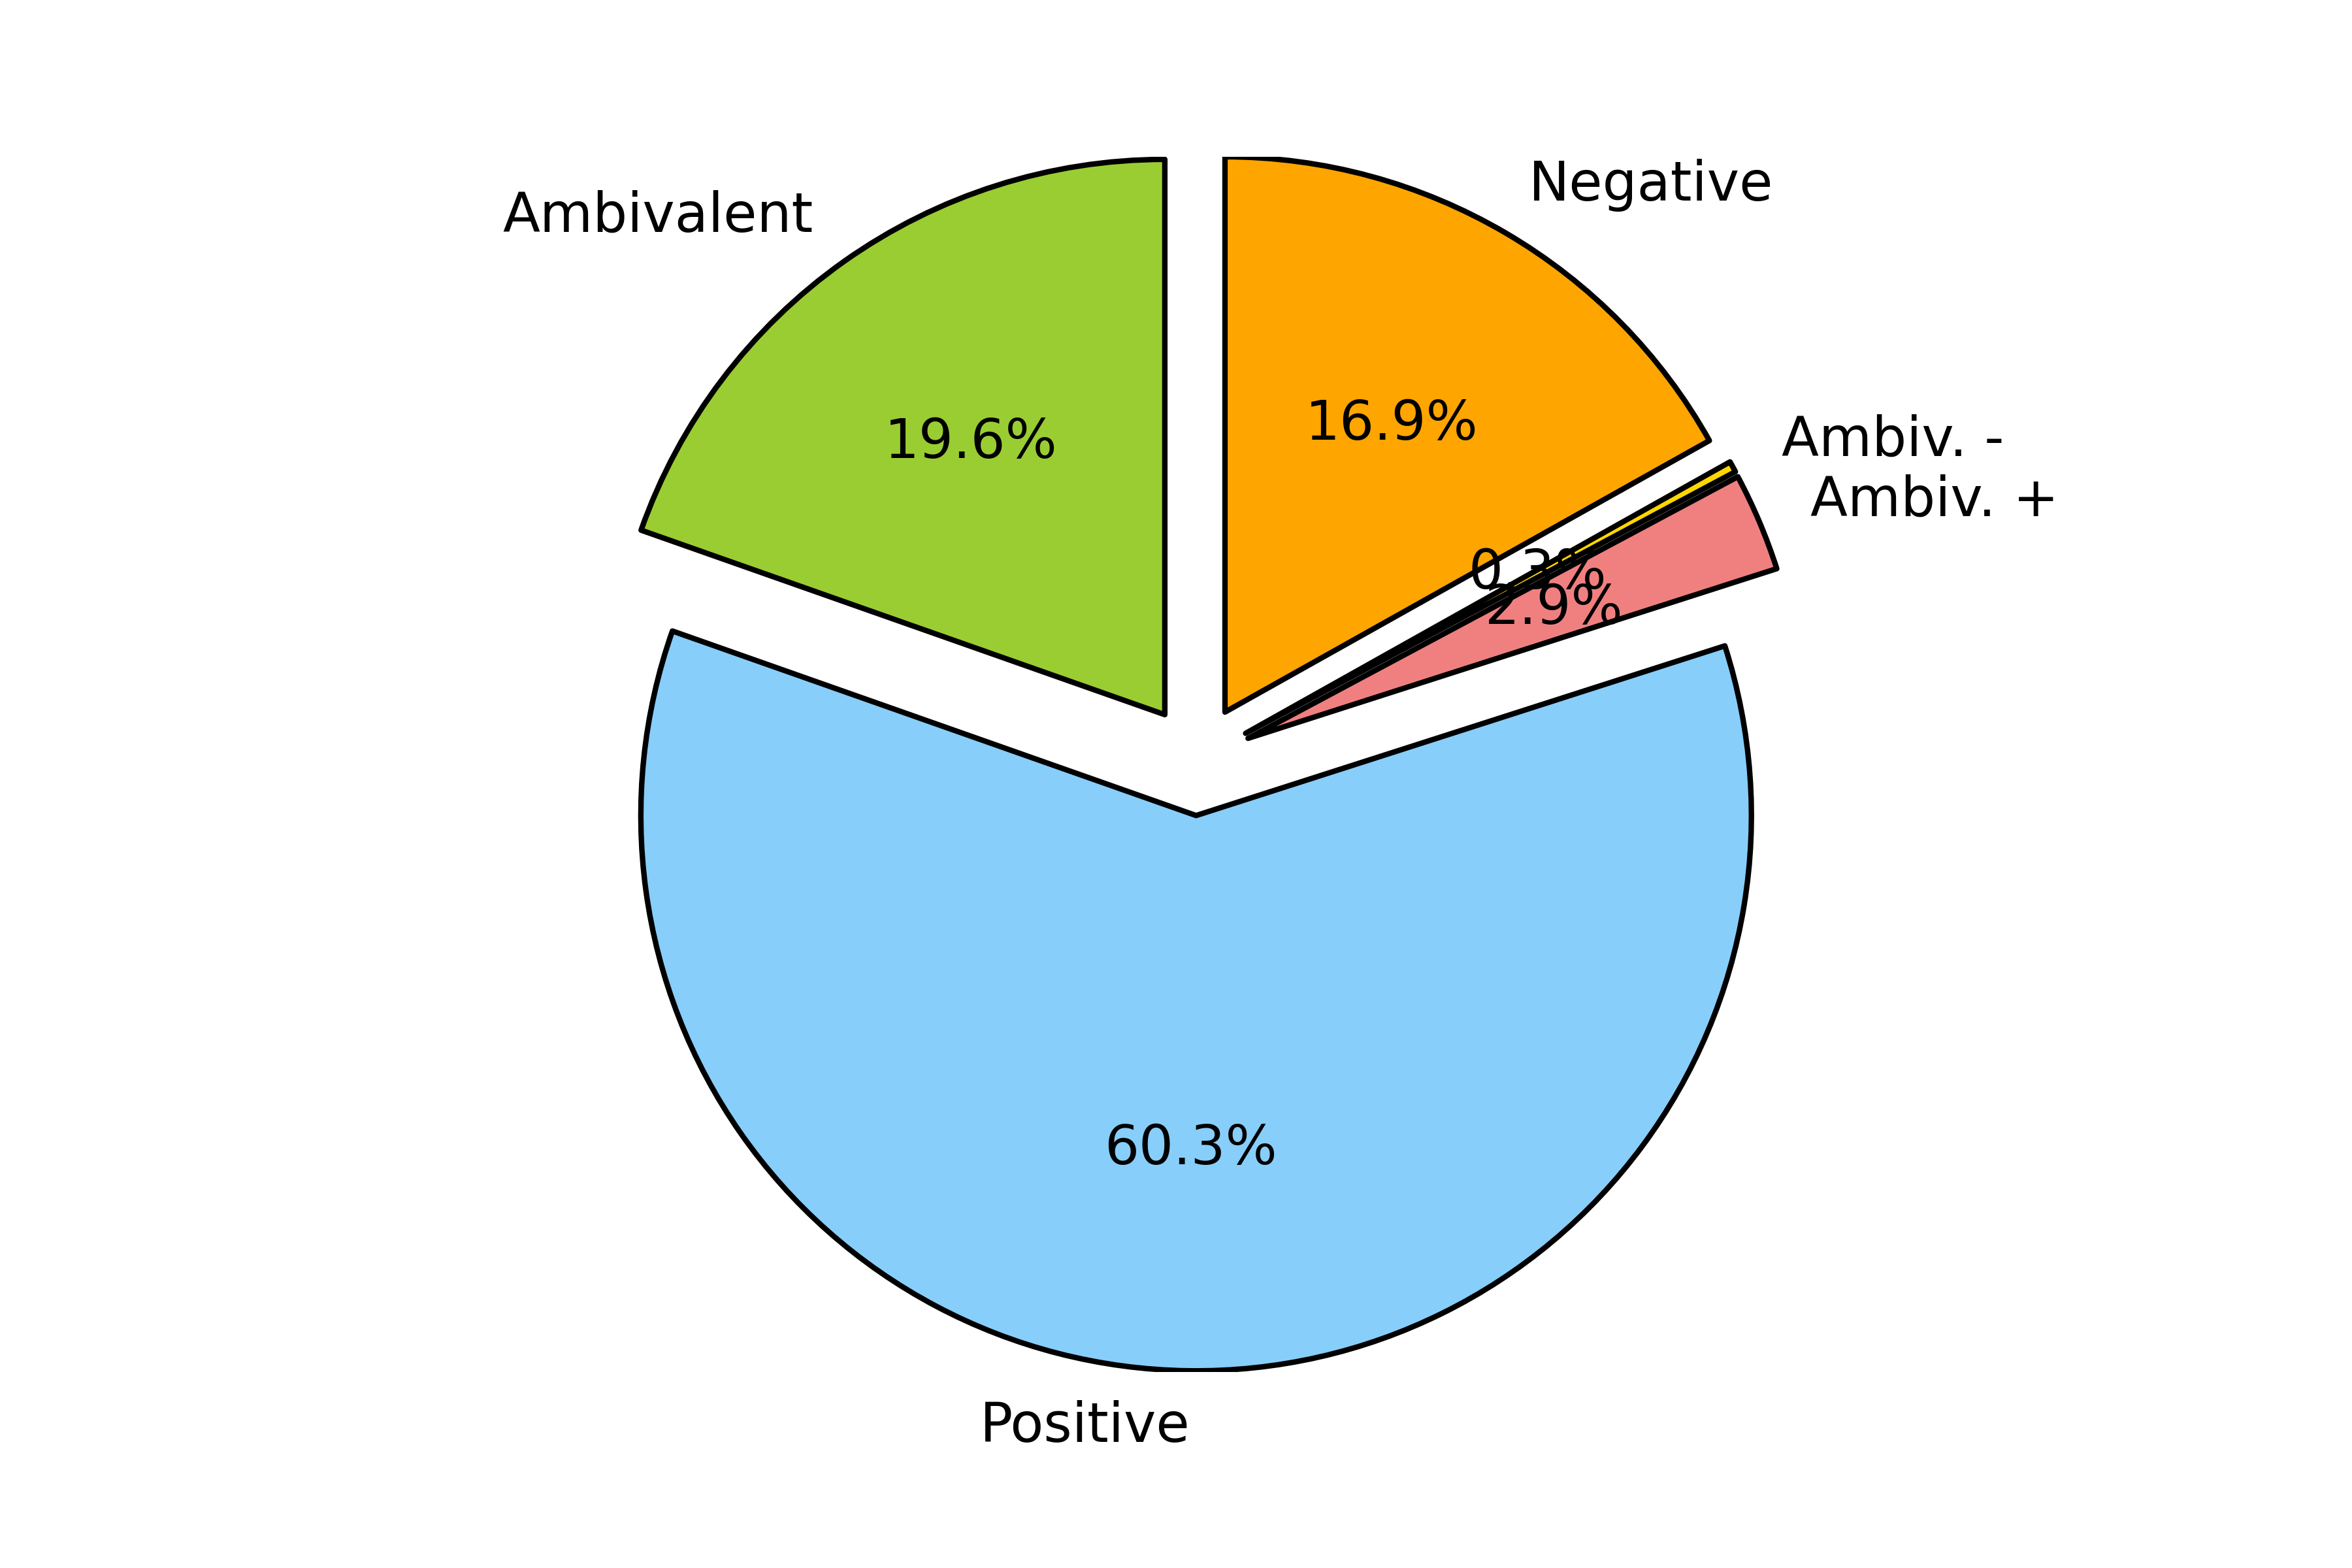
\includegraphics[trim = 1.5cm 0 1.5cm 0, clip = true, width=\textwidth]{../result/charts/emotion_identification_all}
		\caption{总体}
	\end{subfigure}
	\begin{subfigure}[b]{0.3\linewidth}
		\centering
		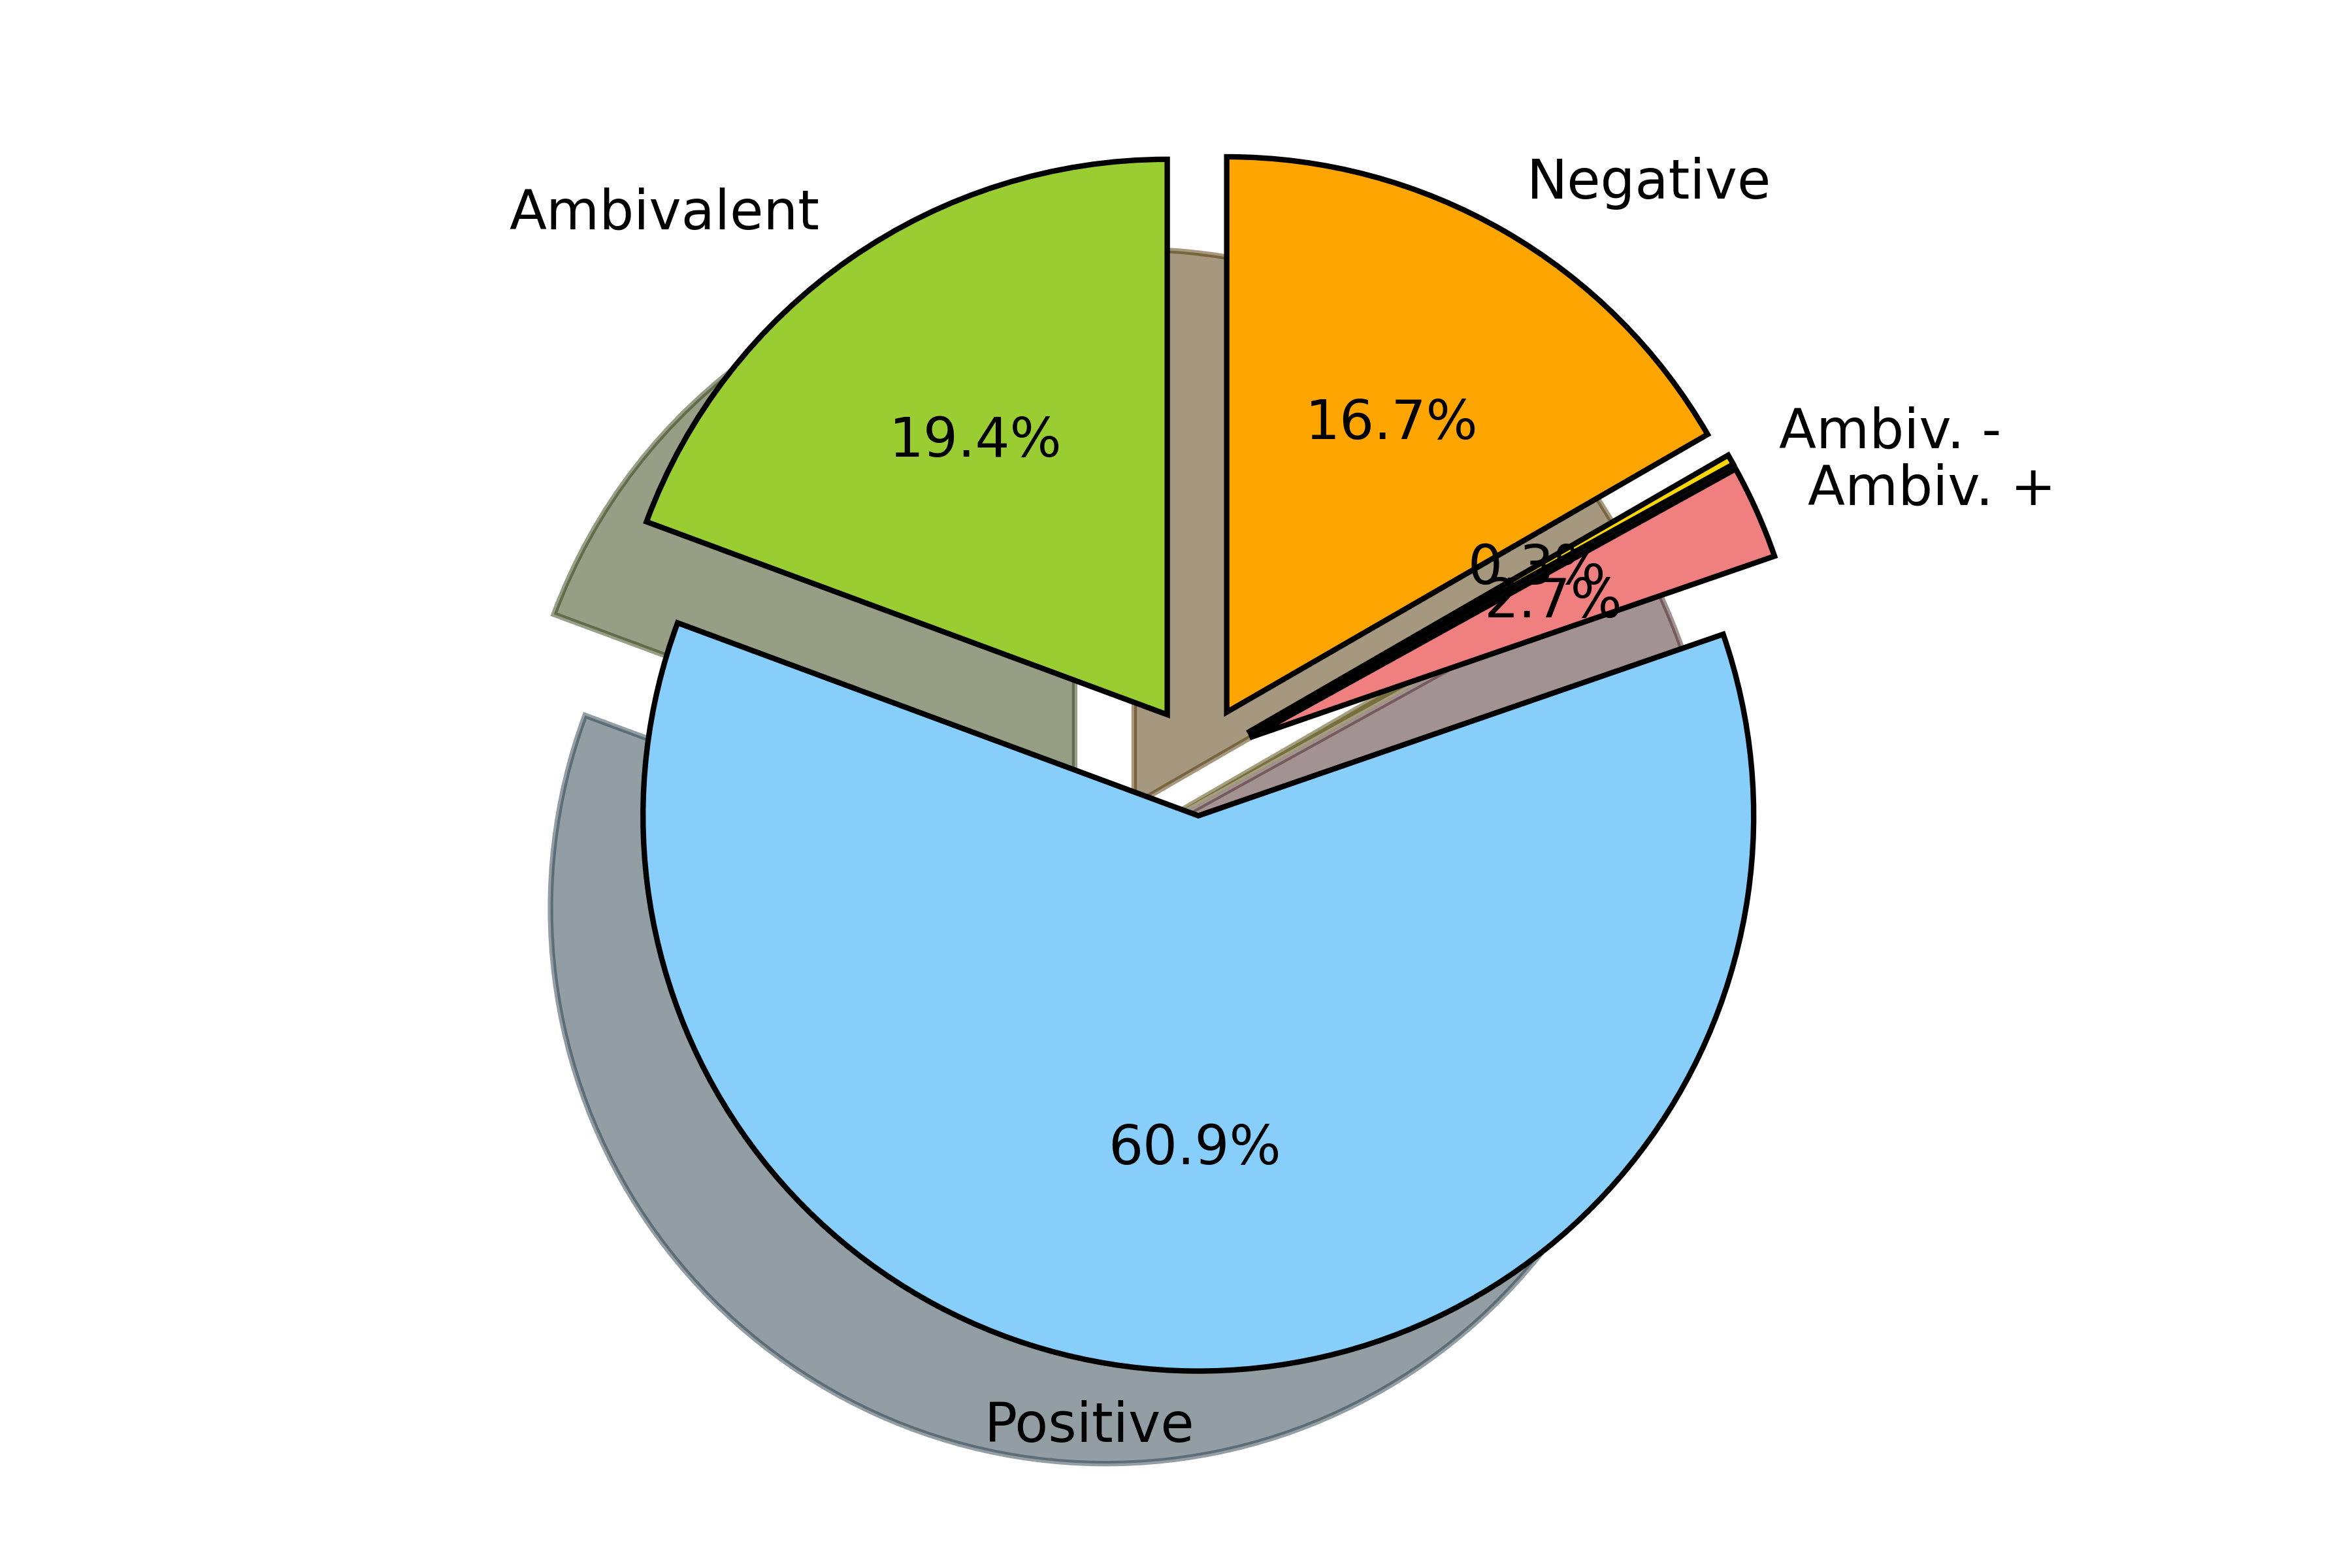
\includegraphics[trim = 1.5cm 0 1.5cm 0, clip = true, width=\textwidth]{../result/charts/emotion_identification_ordinary}
		\caption{普通用户}
	\end{subfigure}
	\begin{subfigure}[b]{0.3\linewidth}
		\centering
		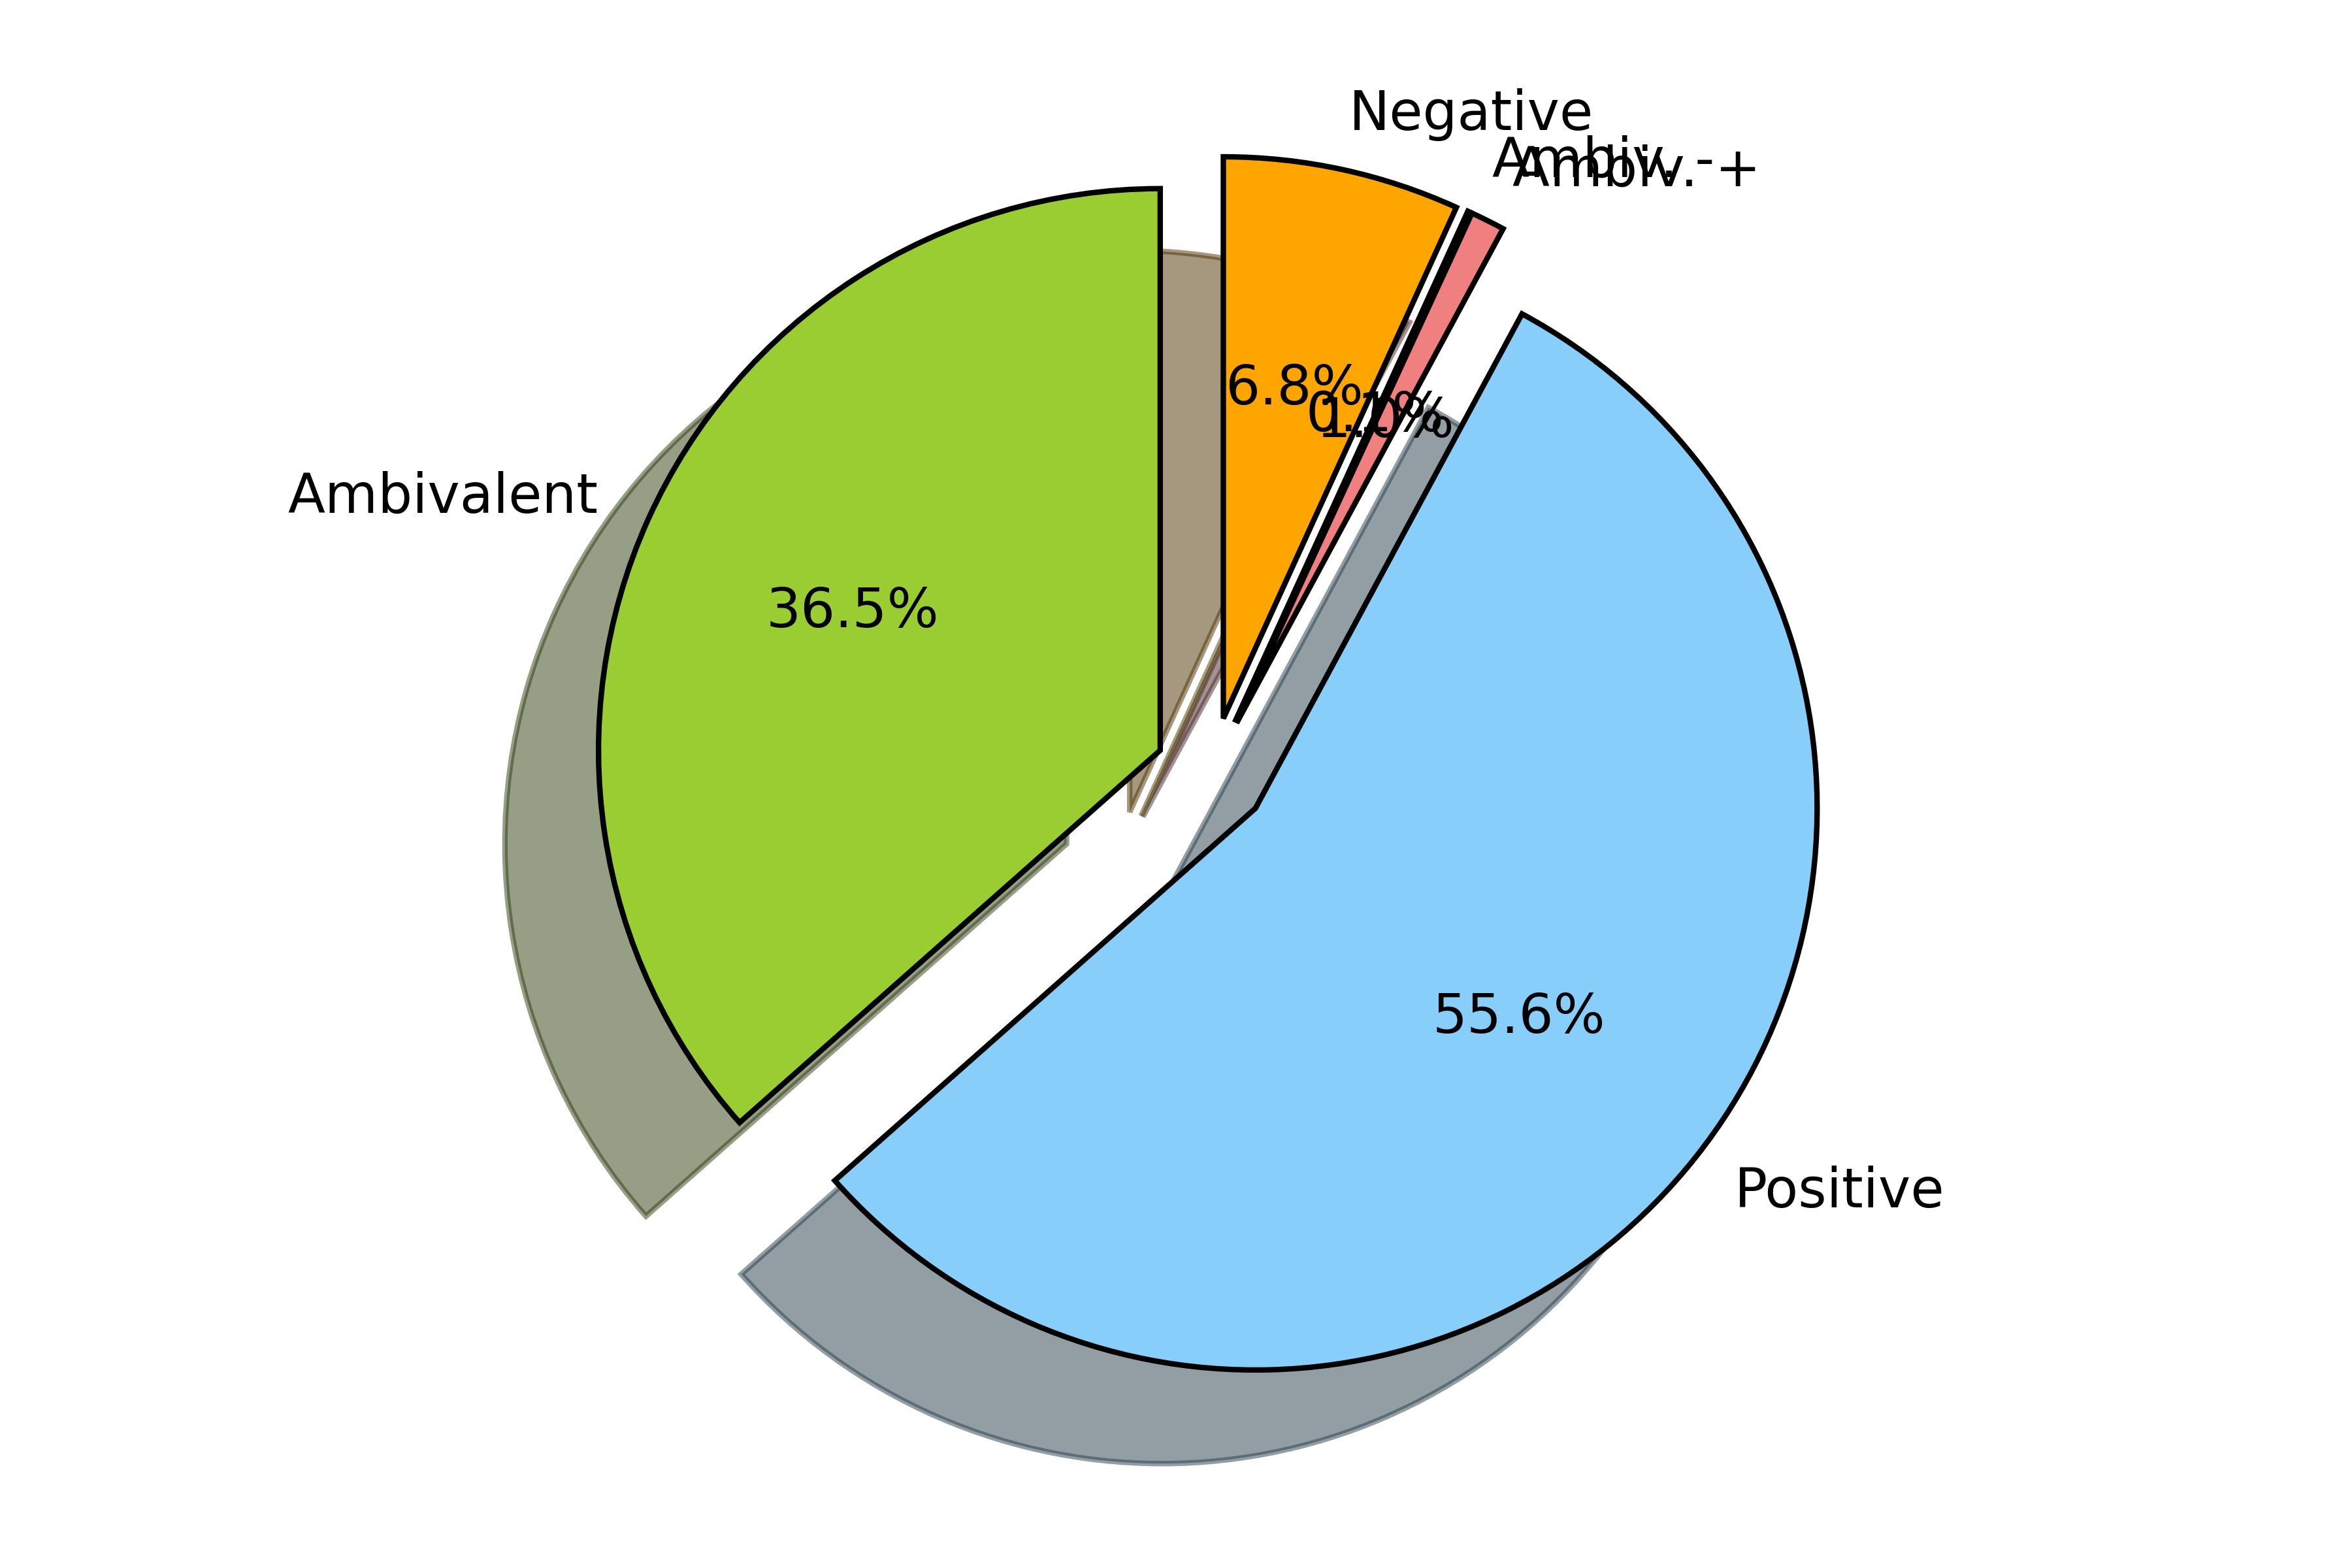
\includegraphics[trim = 1.5cm 0 1.5cm 0, clip = true, width=\textwidth]{../result/charts/emotion_identification_government}
		\caption{政府}
	\end{subfigure}
	\\
	\begin{subfigure}[b]{0.3\linewidth}
		\centering
		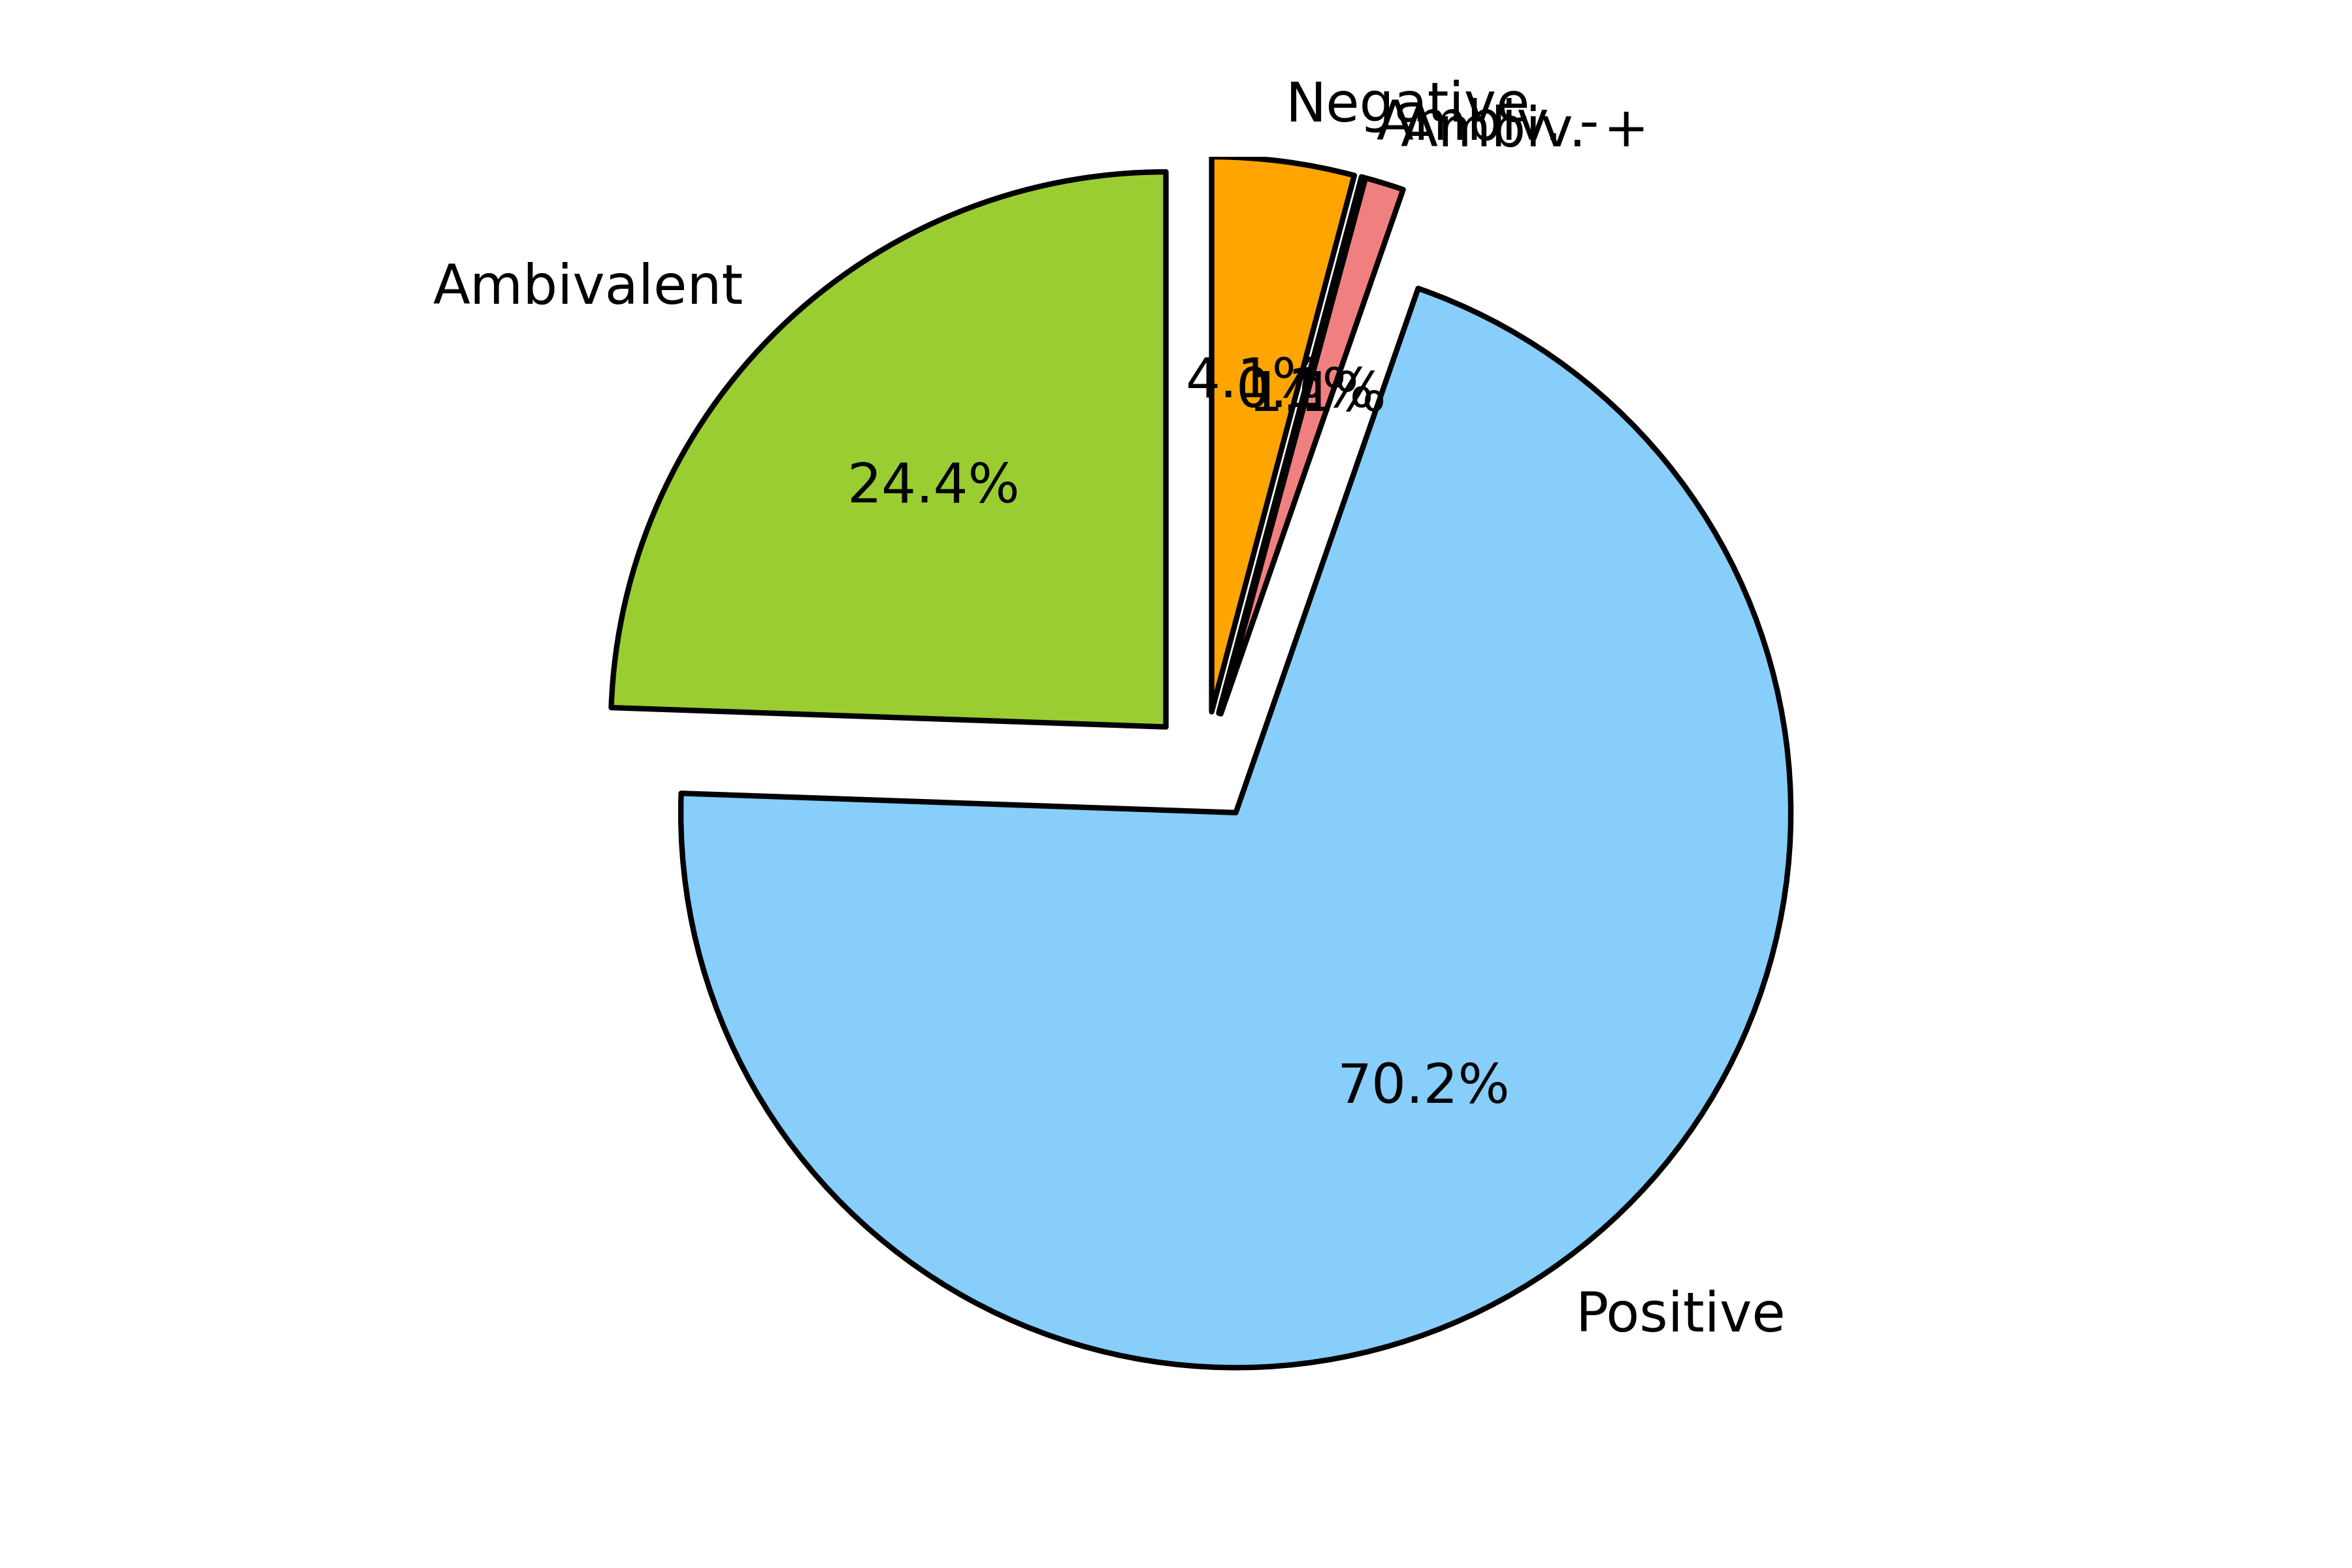
\includegraphics[trim = 1.5cm 0 1.5cm 0, clip = true, width=\textwidth]{../result/charts/emotion_identification_campus}
		\caption{学校}
	\end{subfigure}
	\begin{subfigure}[b]{0.3\linewidth}
		\centering
		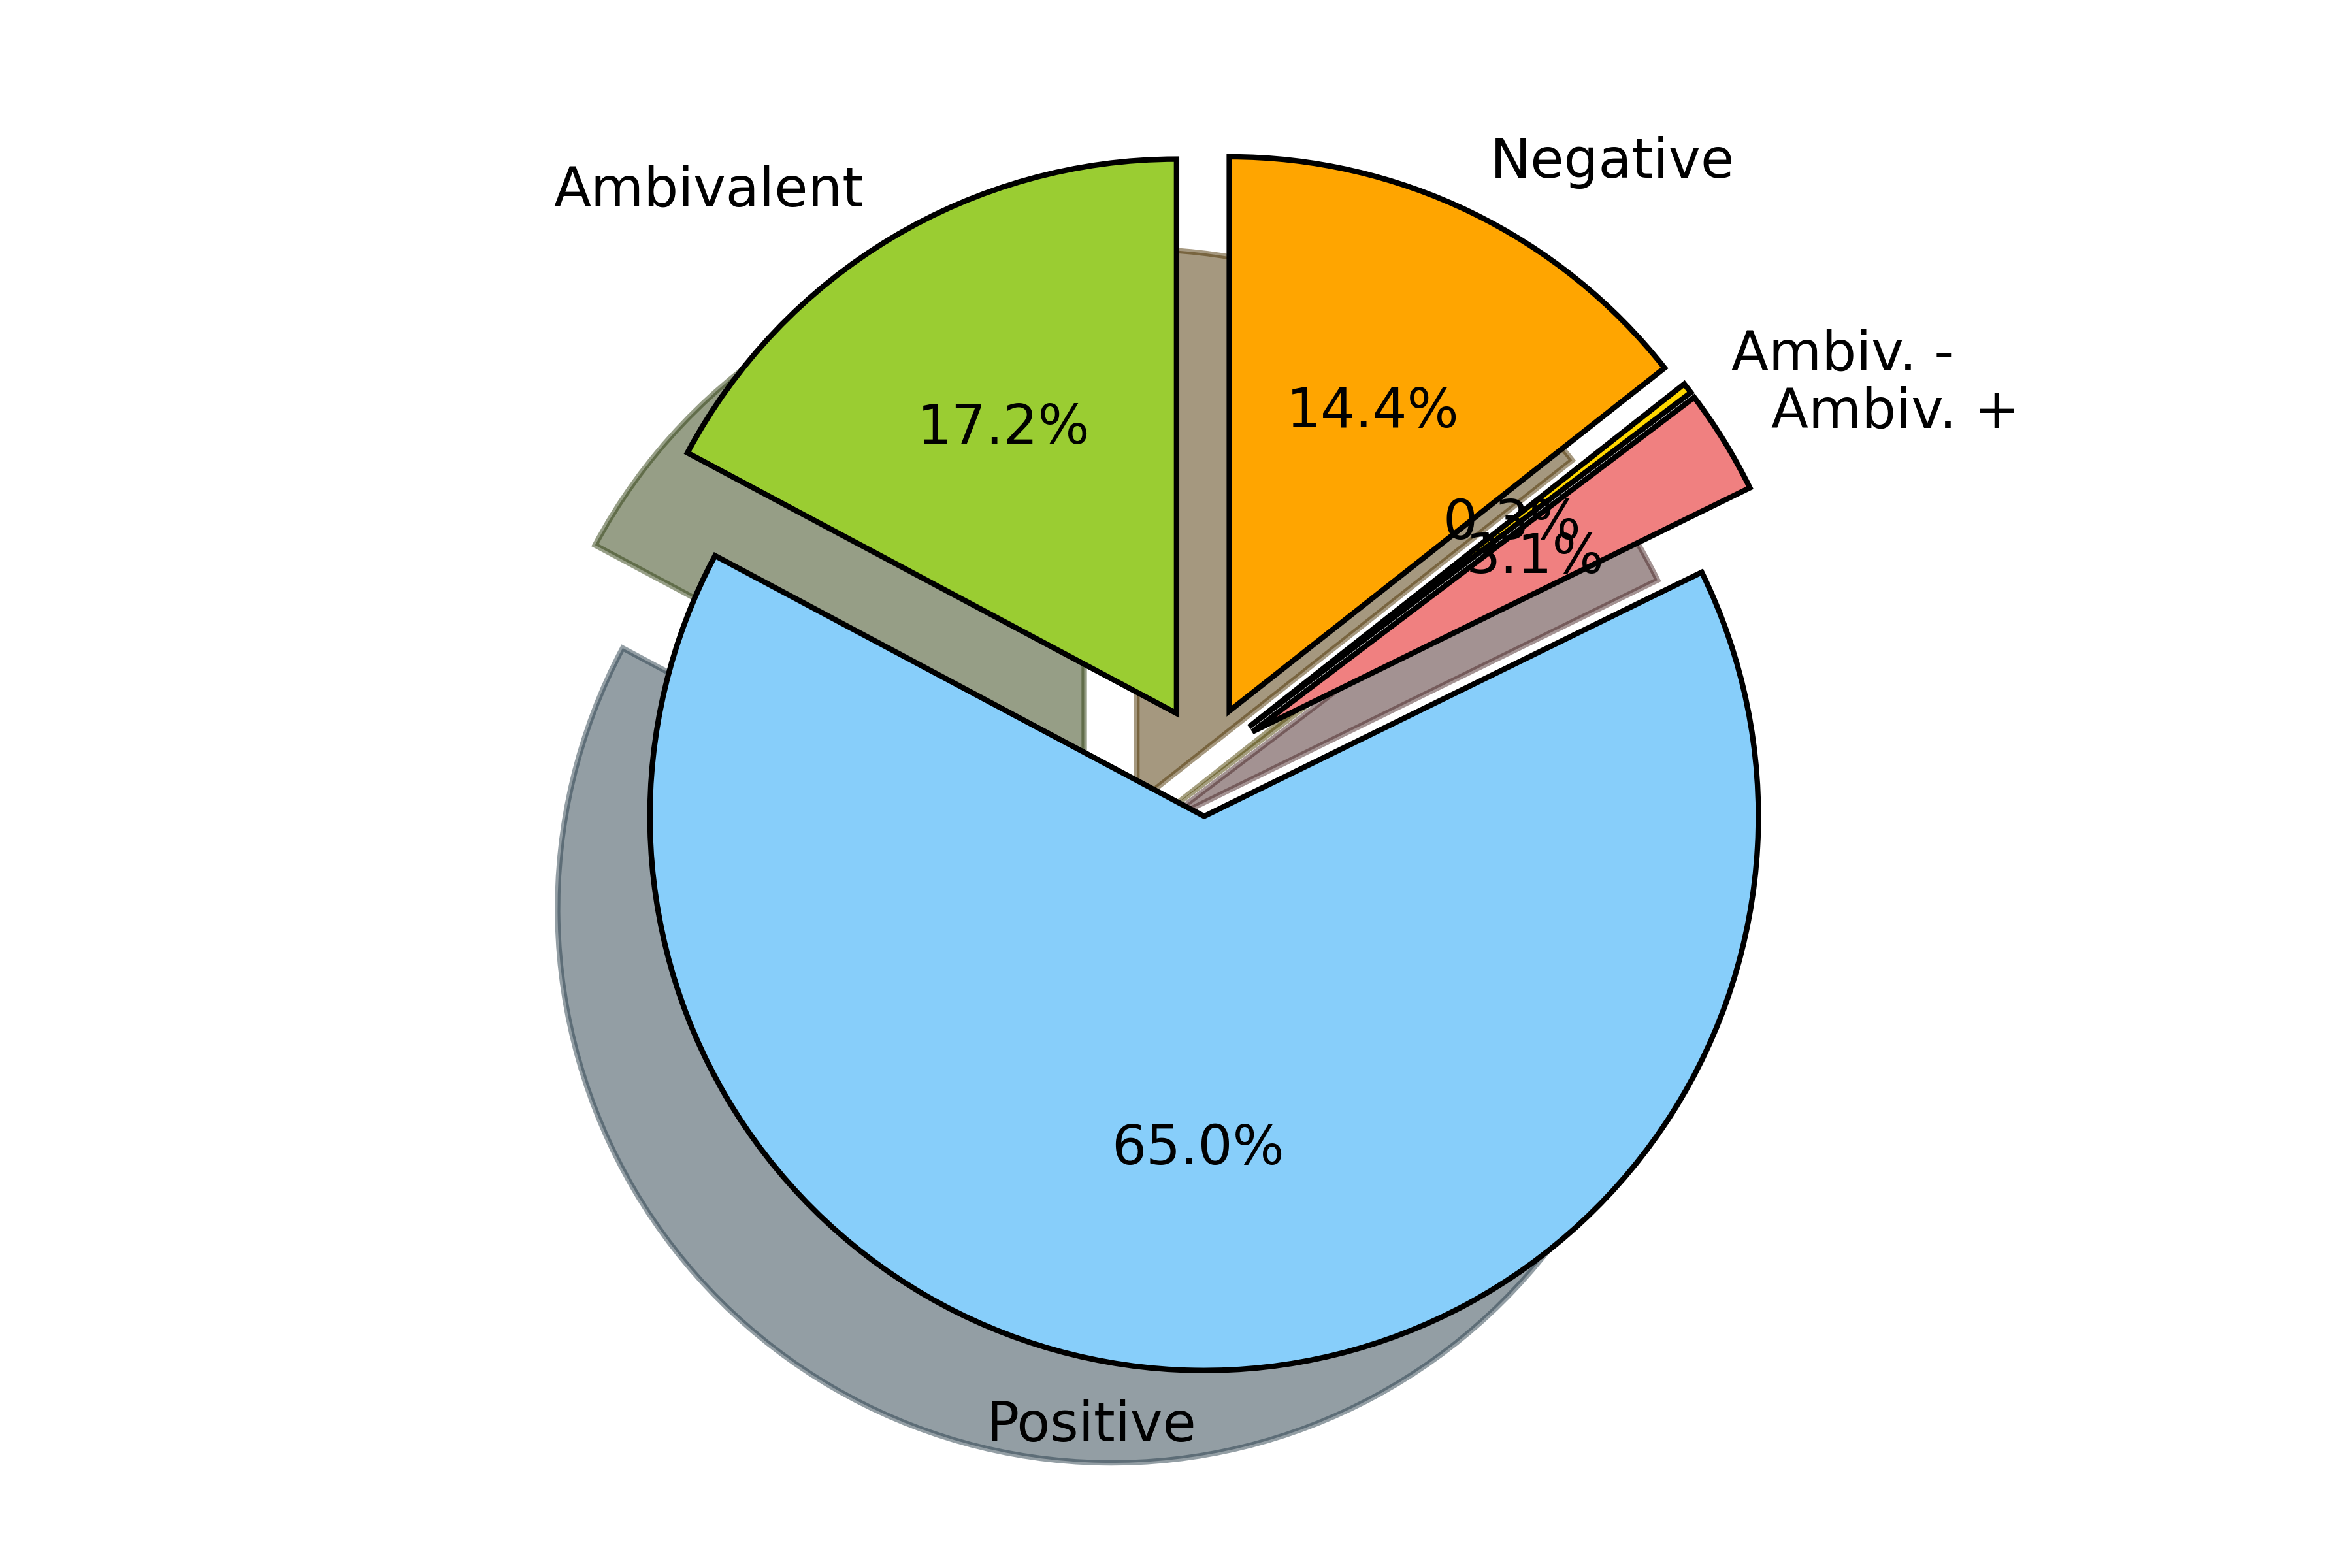
\includegraphics[trim = 1.5cm 0 1.5cm 0, clip = true, width=\textwidth]{../result/charts/emotion_identification_celebrities}
		\caption{名人}
	\end{subfigure}
	\begin{subfigure}[b]{0.3\linewidth}
		\centering
		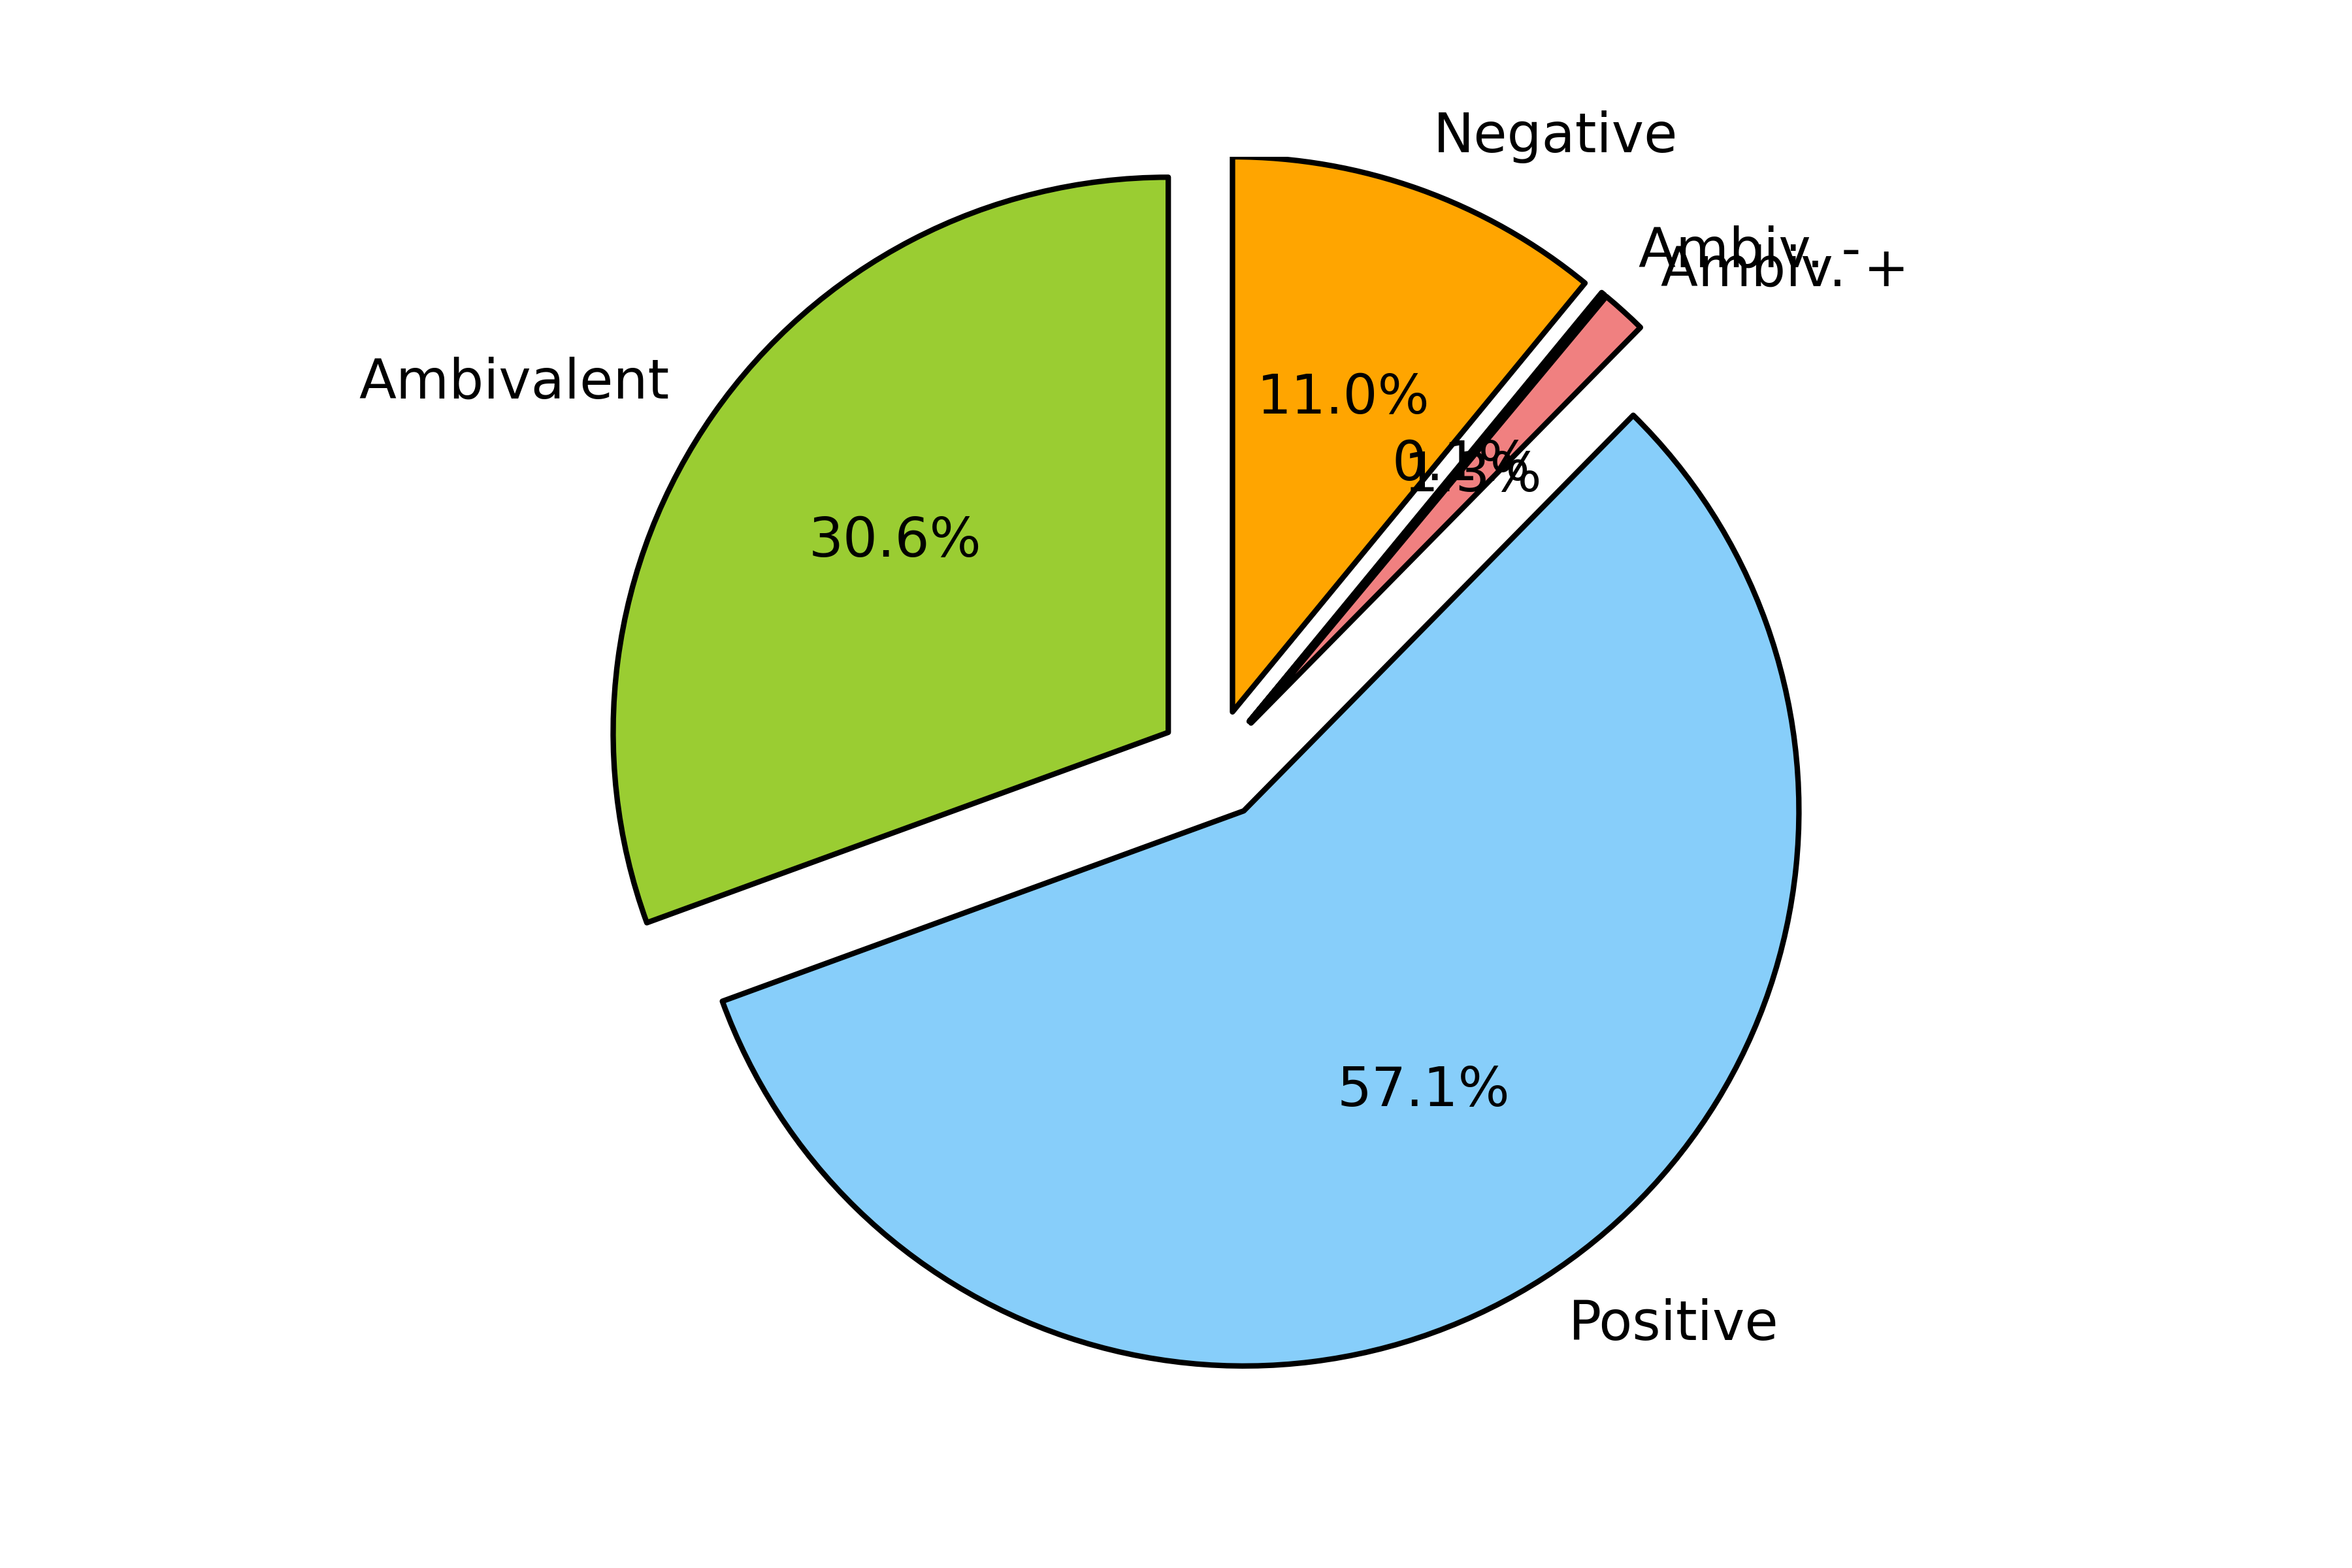
\includegraphics[trim = 1.5cm 0 1.5cm 0, clip = true, width=\textwidth]{../result/charts/emotion_identification_media}
		\caption{媒体}
	\end{subfigure}
	\\
	\begin{subfigure}[b]{0.3\linewidth}
		\centering
		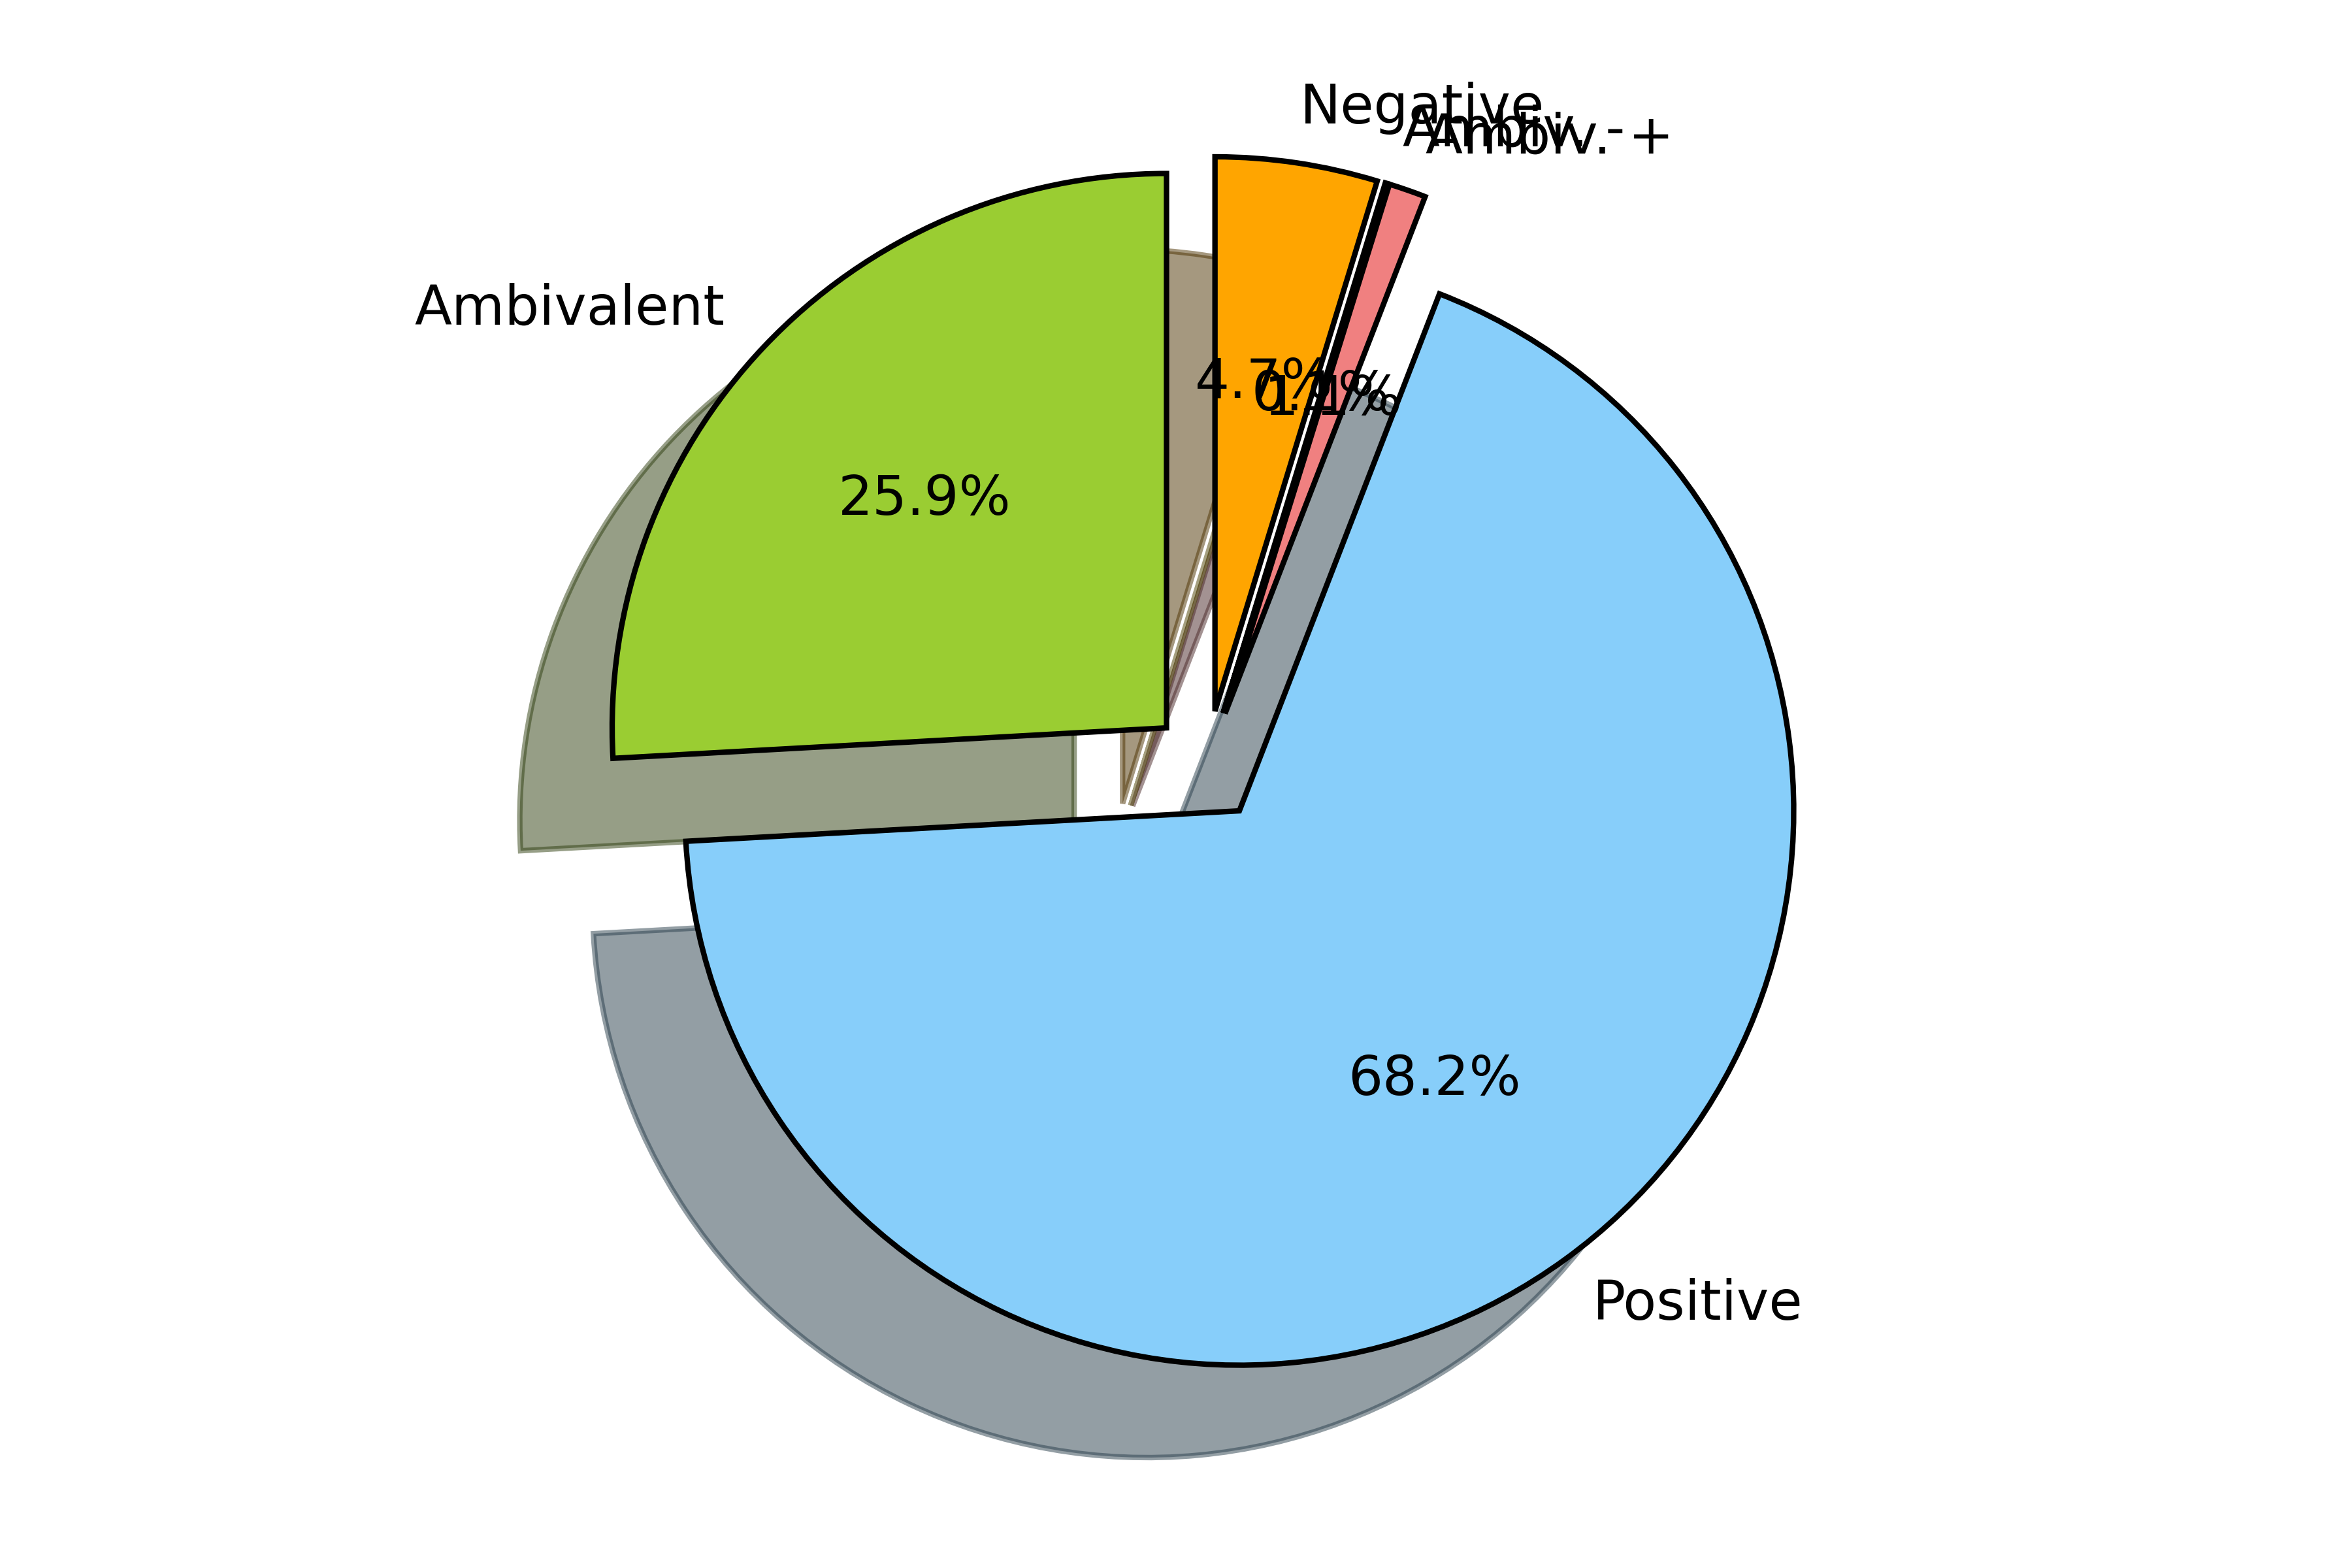
\includegraphics[trim = 1.5cm 0 1.5cm 0, clip = true, width=\textwidth]{../result/charts/emotion_identification_enterprises}
		\caption{企业}
	\end{subfigure}
	\begin{subfigure}[b]{0.3\linewidth}
		\centering
		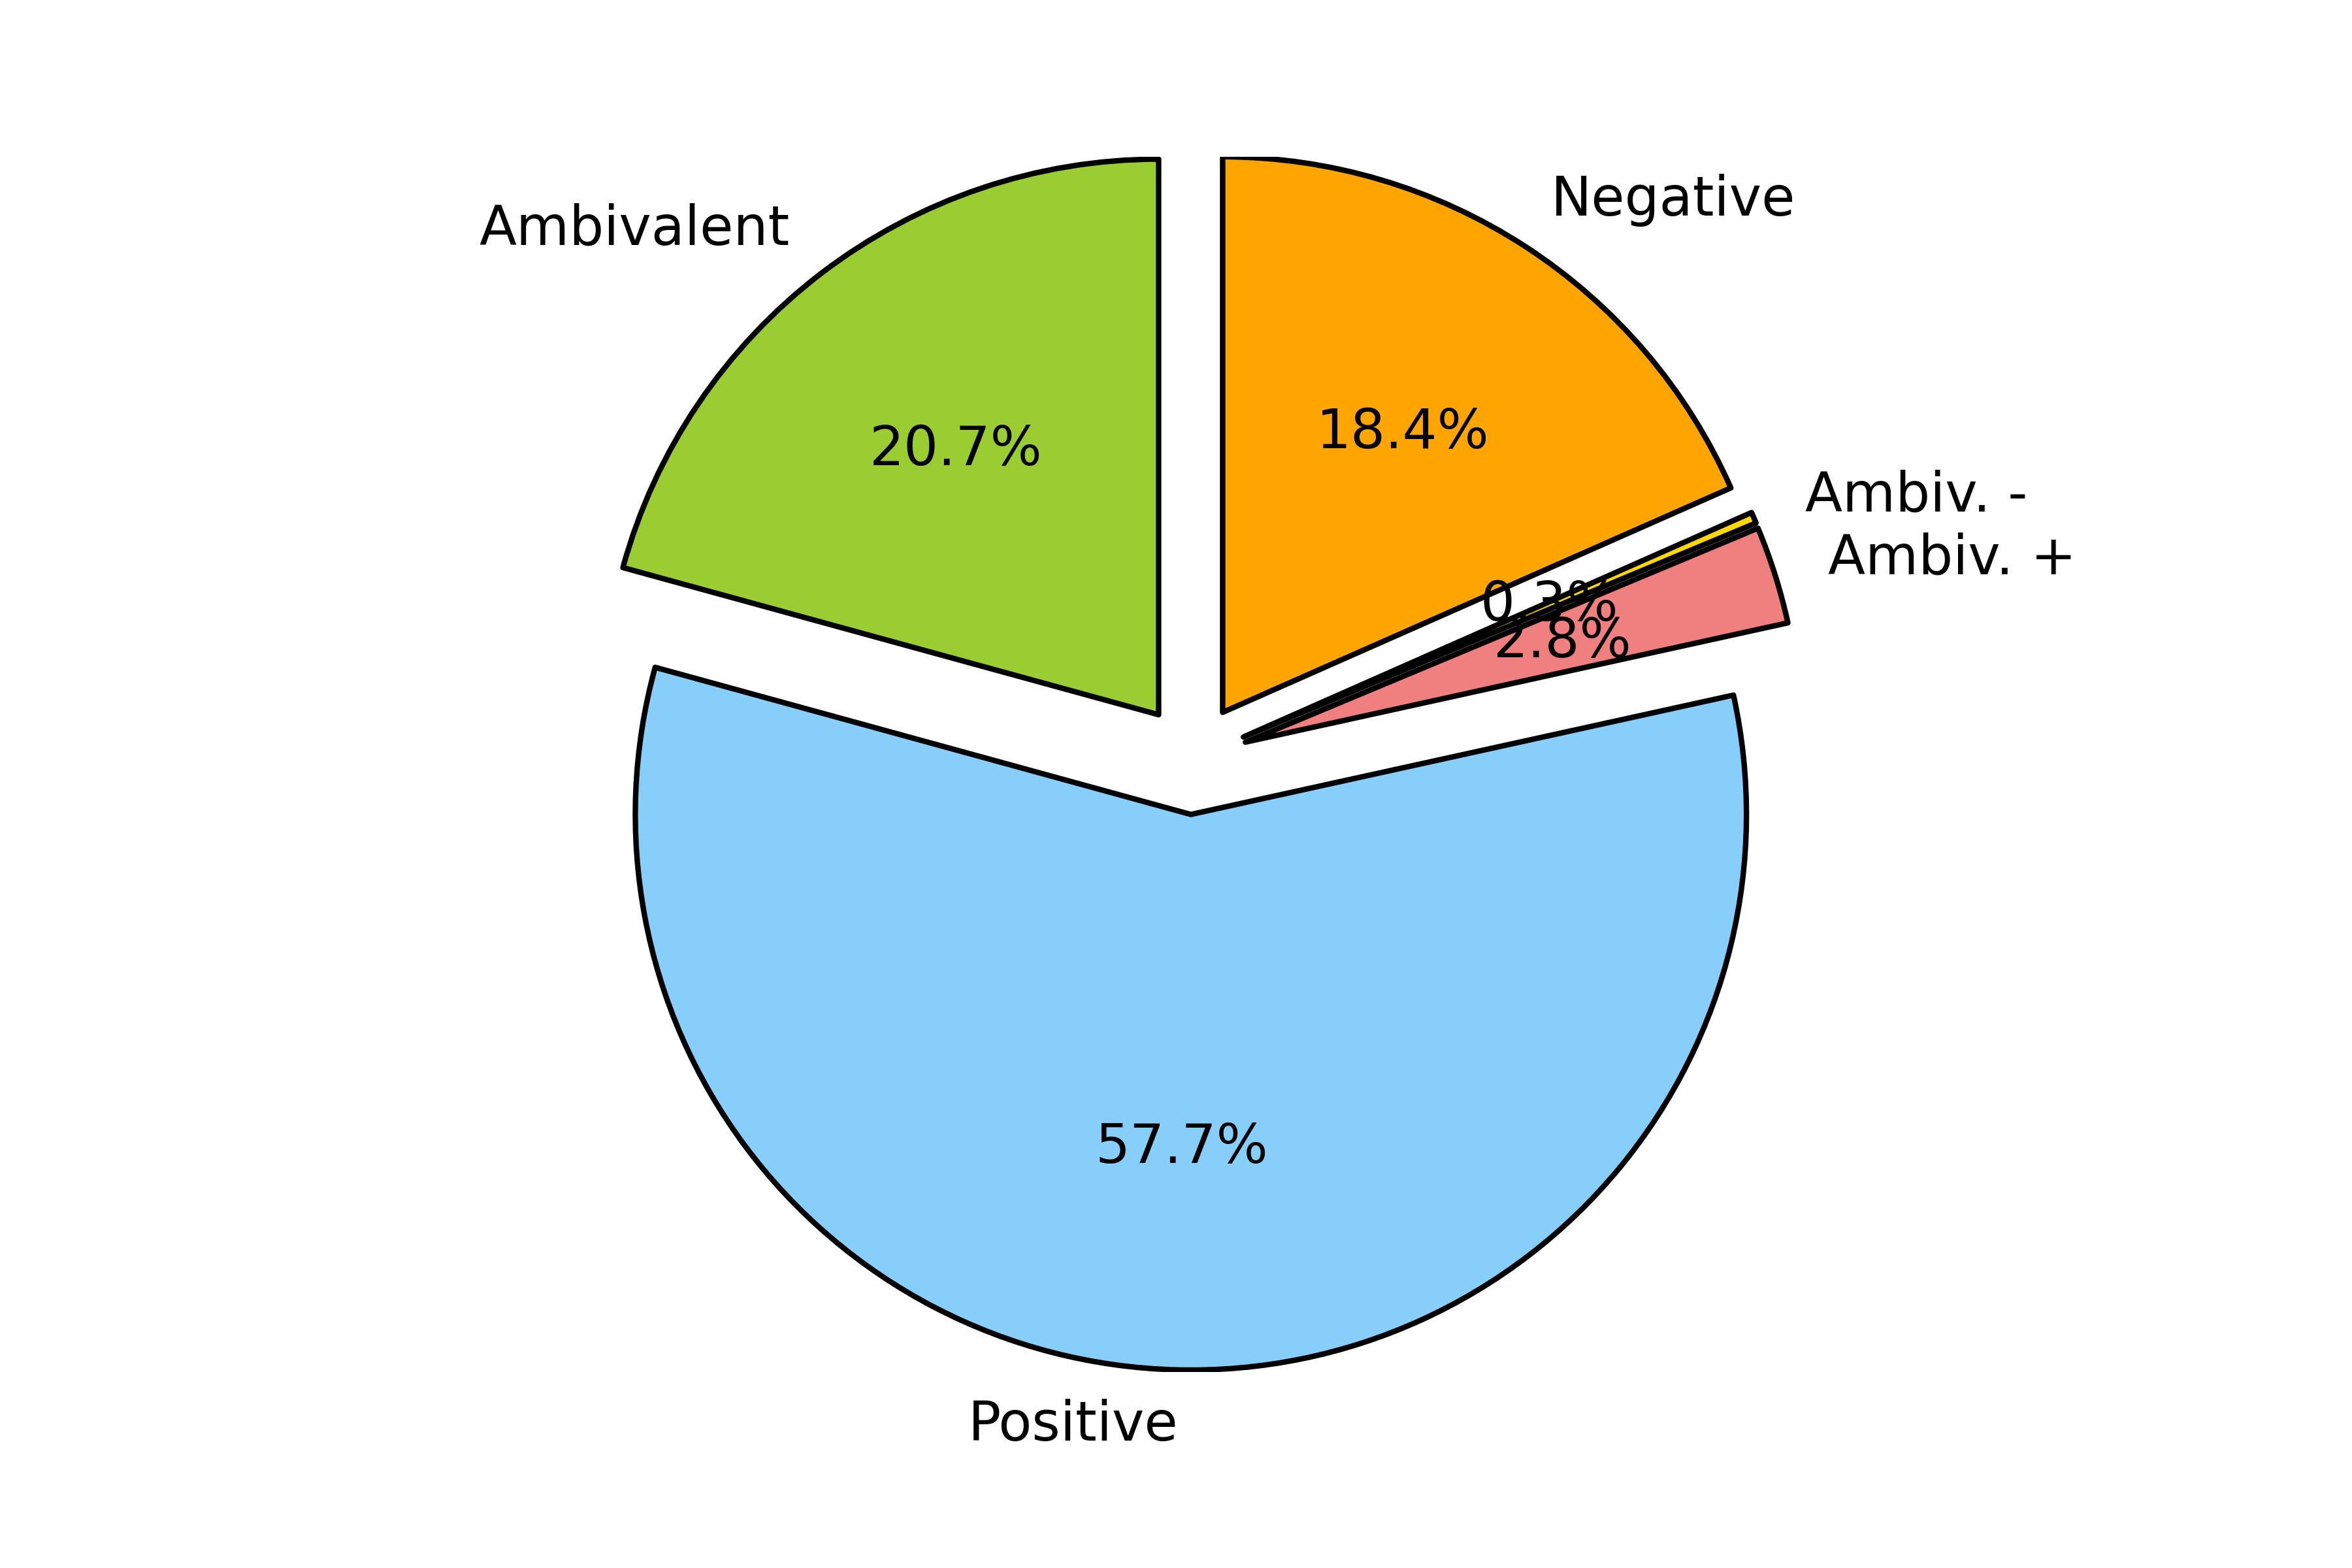
\includegraphics[trim = 1.5cm 0 1.5cm 0, clip = true, width=\textwidth]{../result/charts/emotion_identification_junior}
		\caption{普通会员}
	\end{subfigure}
	\begin{subfigure}[b]{0.3\linewidth}
		\centering
		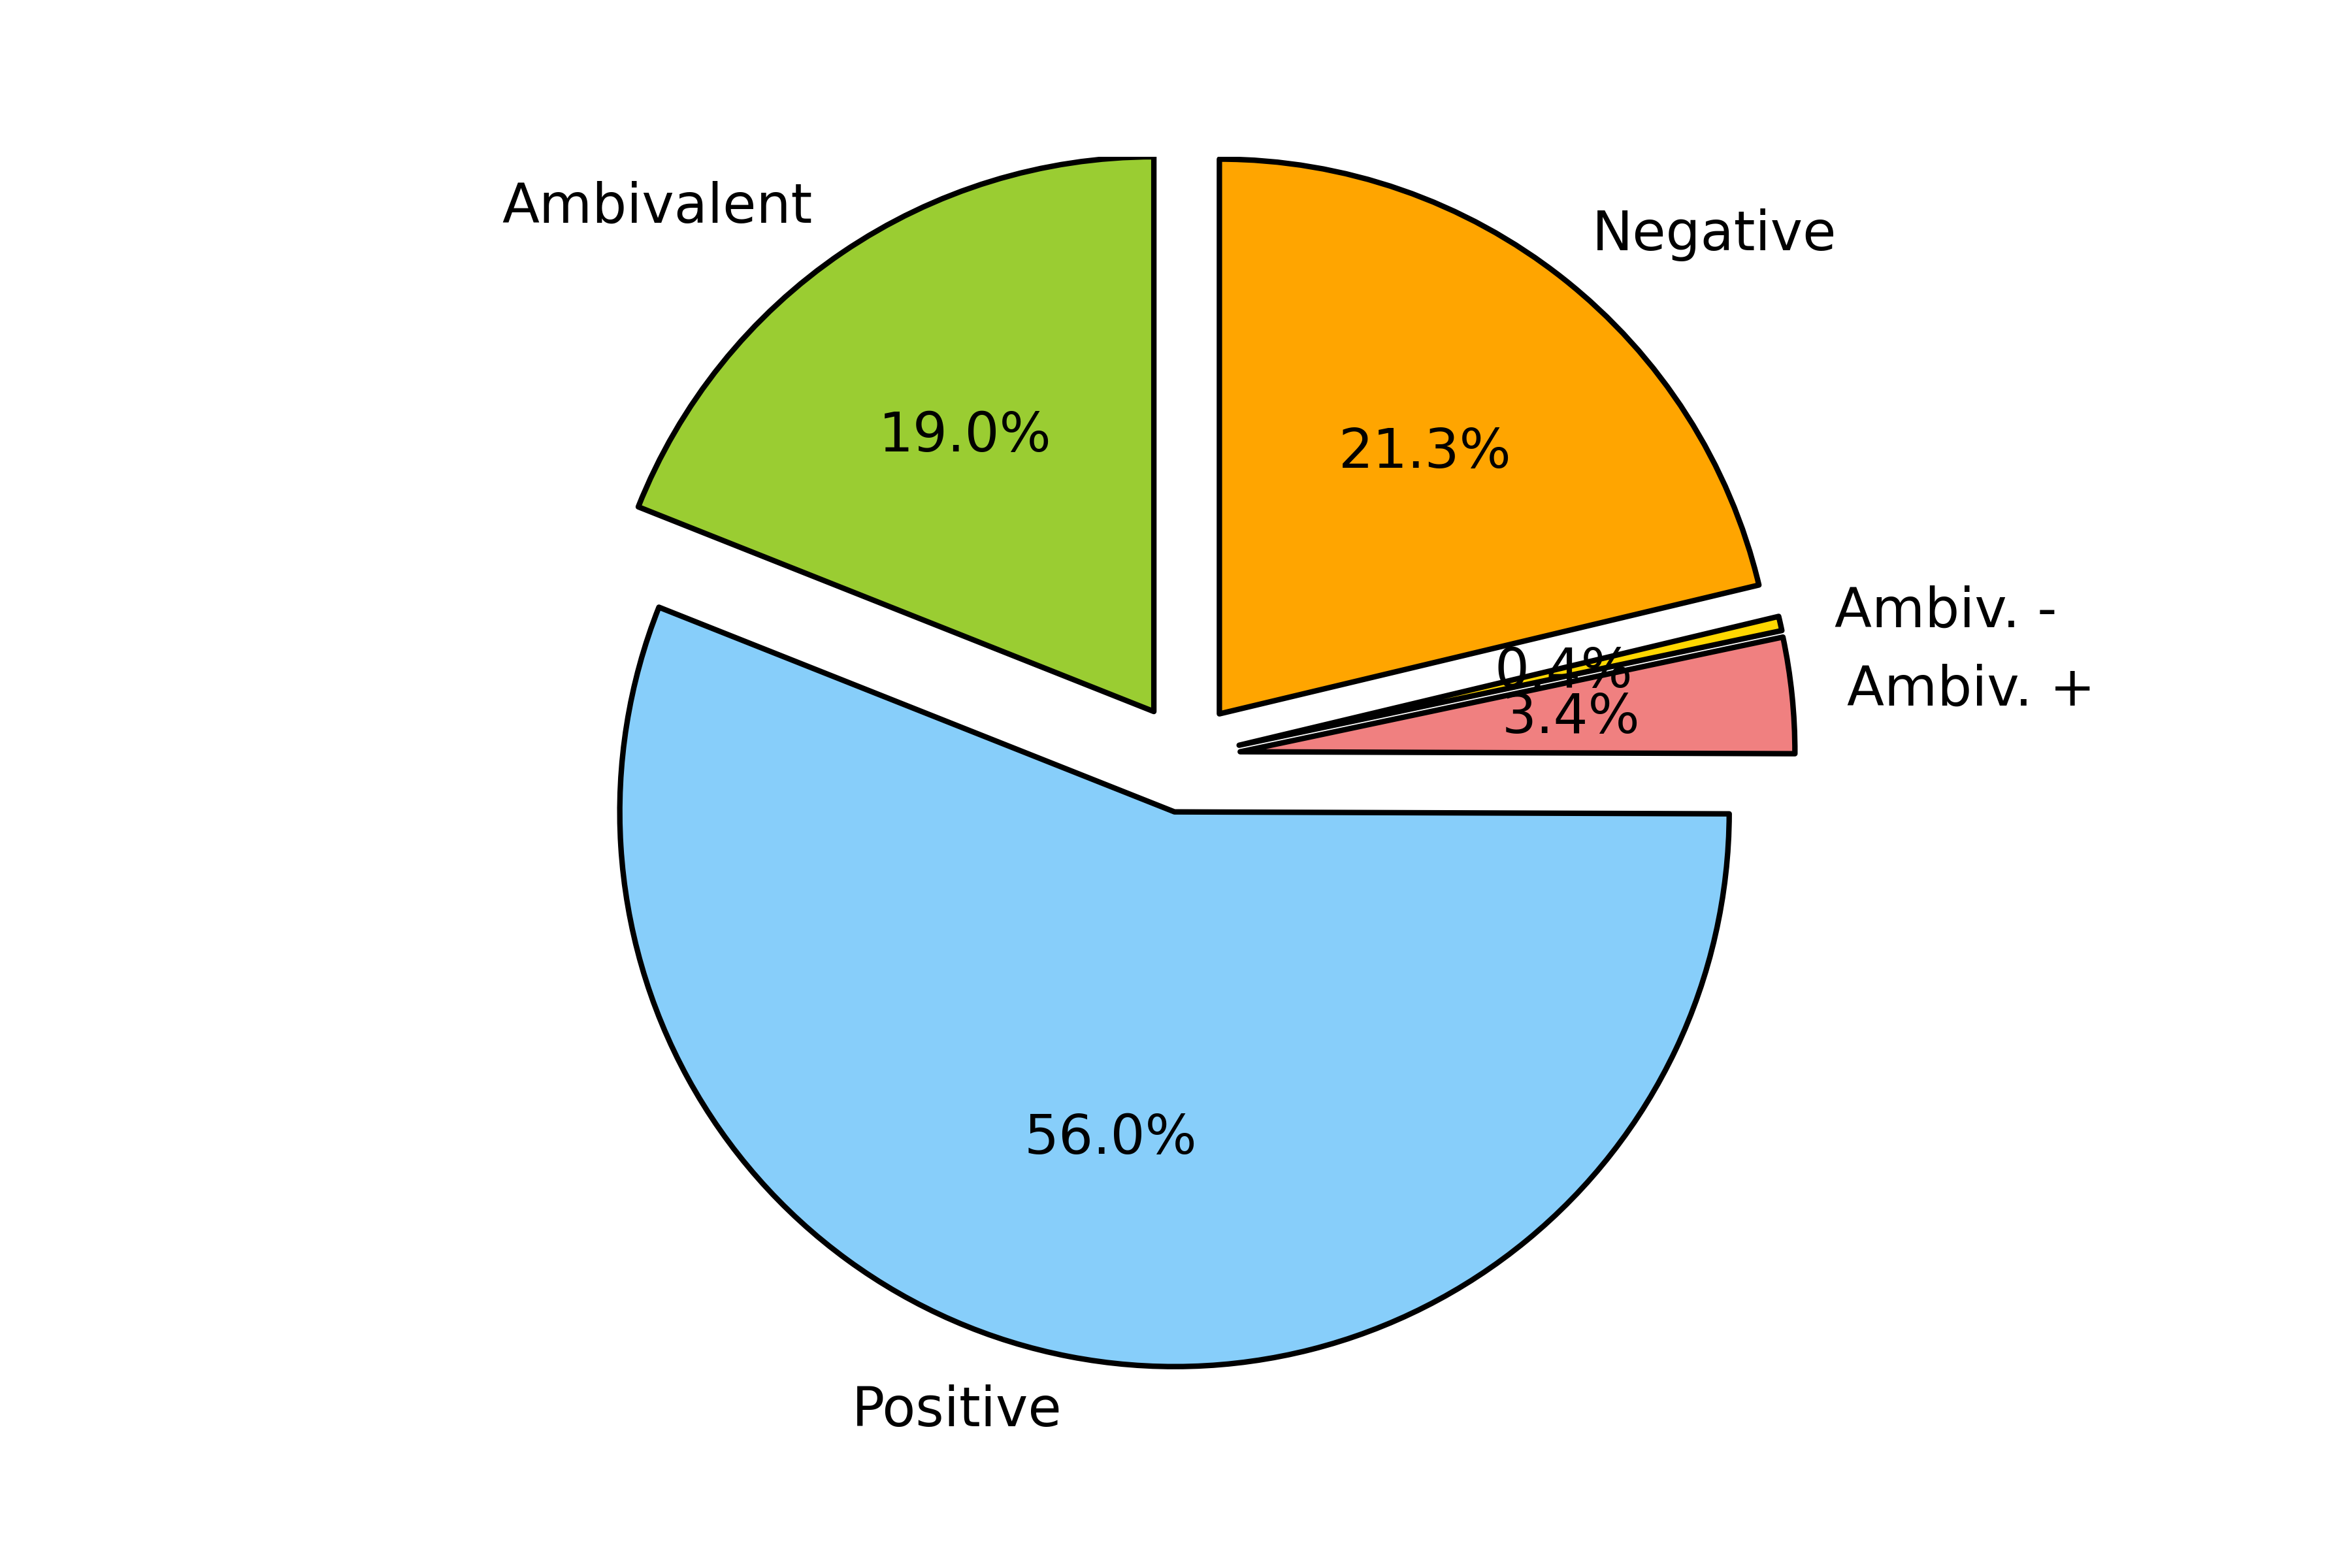
\includegraphics[trim = 1.5cm 0 1.5cm 0, clip = true, width=\textwidth]{../result/charts/emotion_identification_senior}
		\caption{高级会员}
	\end{subfigure}
	\caption{不同类别用户的微博的情绪分布。}
	\label{fig:emotion_identification}
\end{figure}


\subsection{微博情绪-转发量}
为了检验什么样的情绪更容易在微博上被传播,我们使用filter过滤出含有转发符号(“//”)的微博。从图\ref{fig:emotion_forward}中可以明显的比较出,积极情绪的微博更容易被转发。

\begin{figure}
	\centering
	\begin{subfigure}[b]{0.45\linewidth}
		\centering
		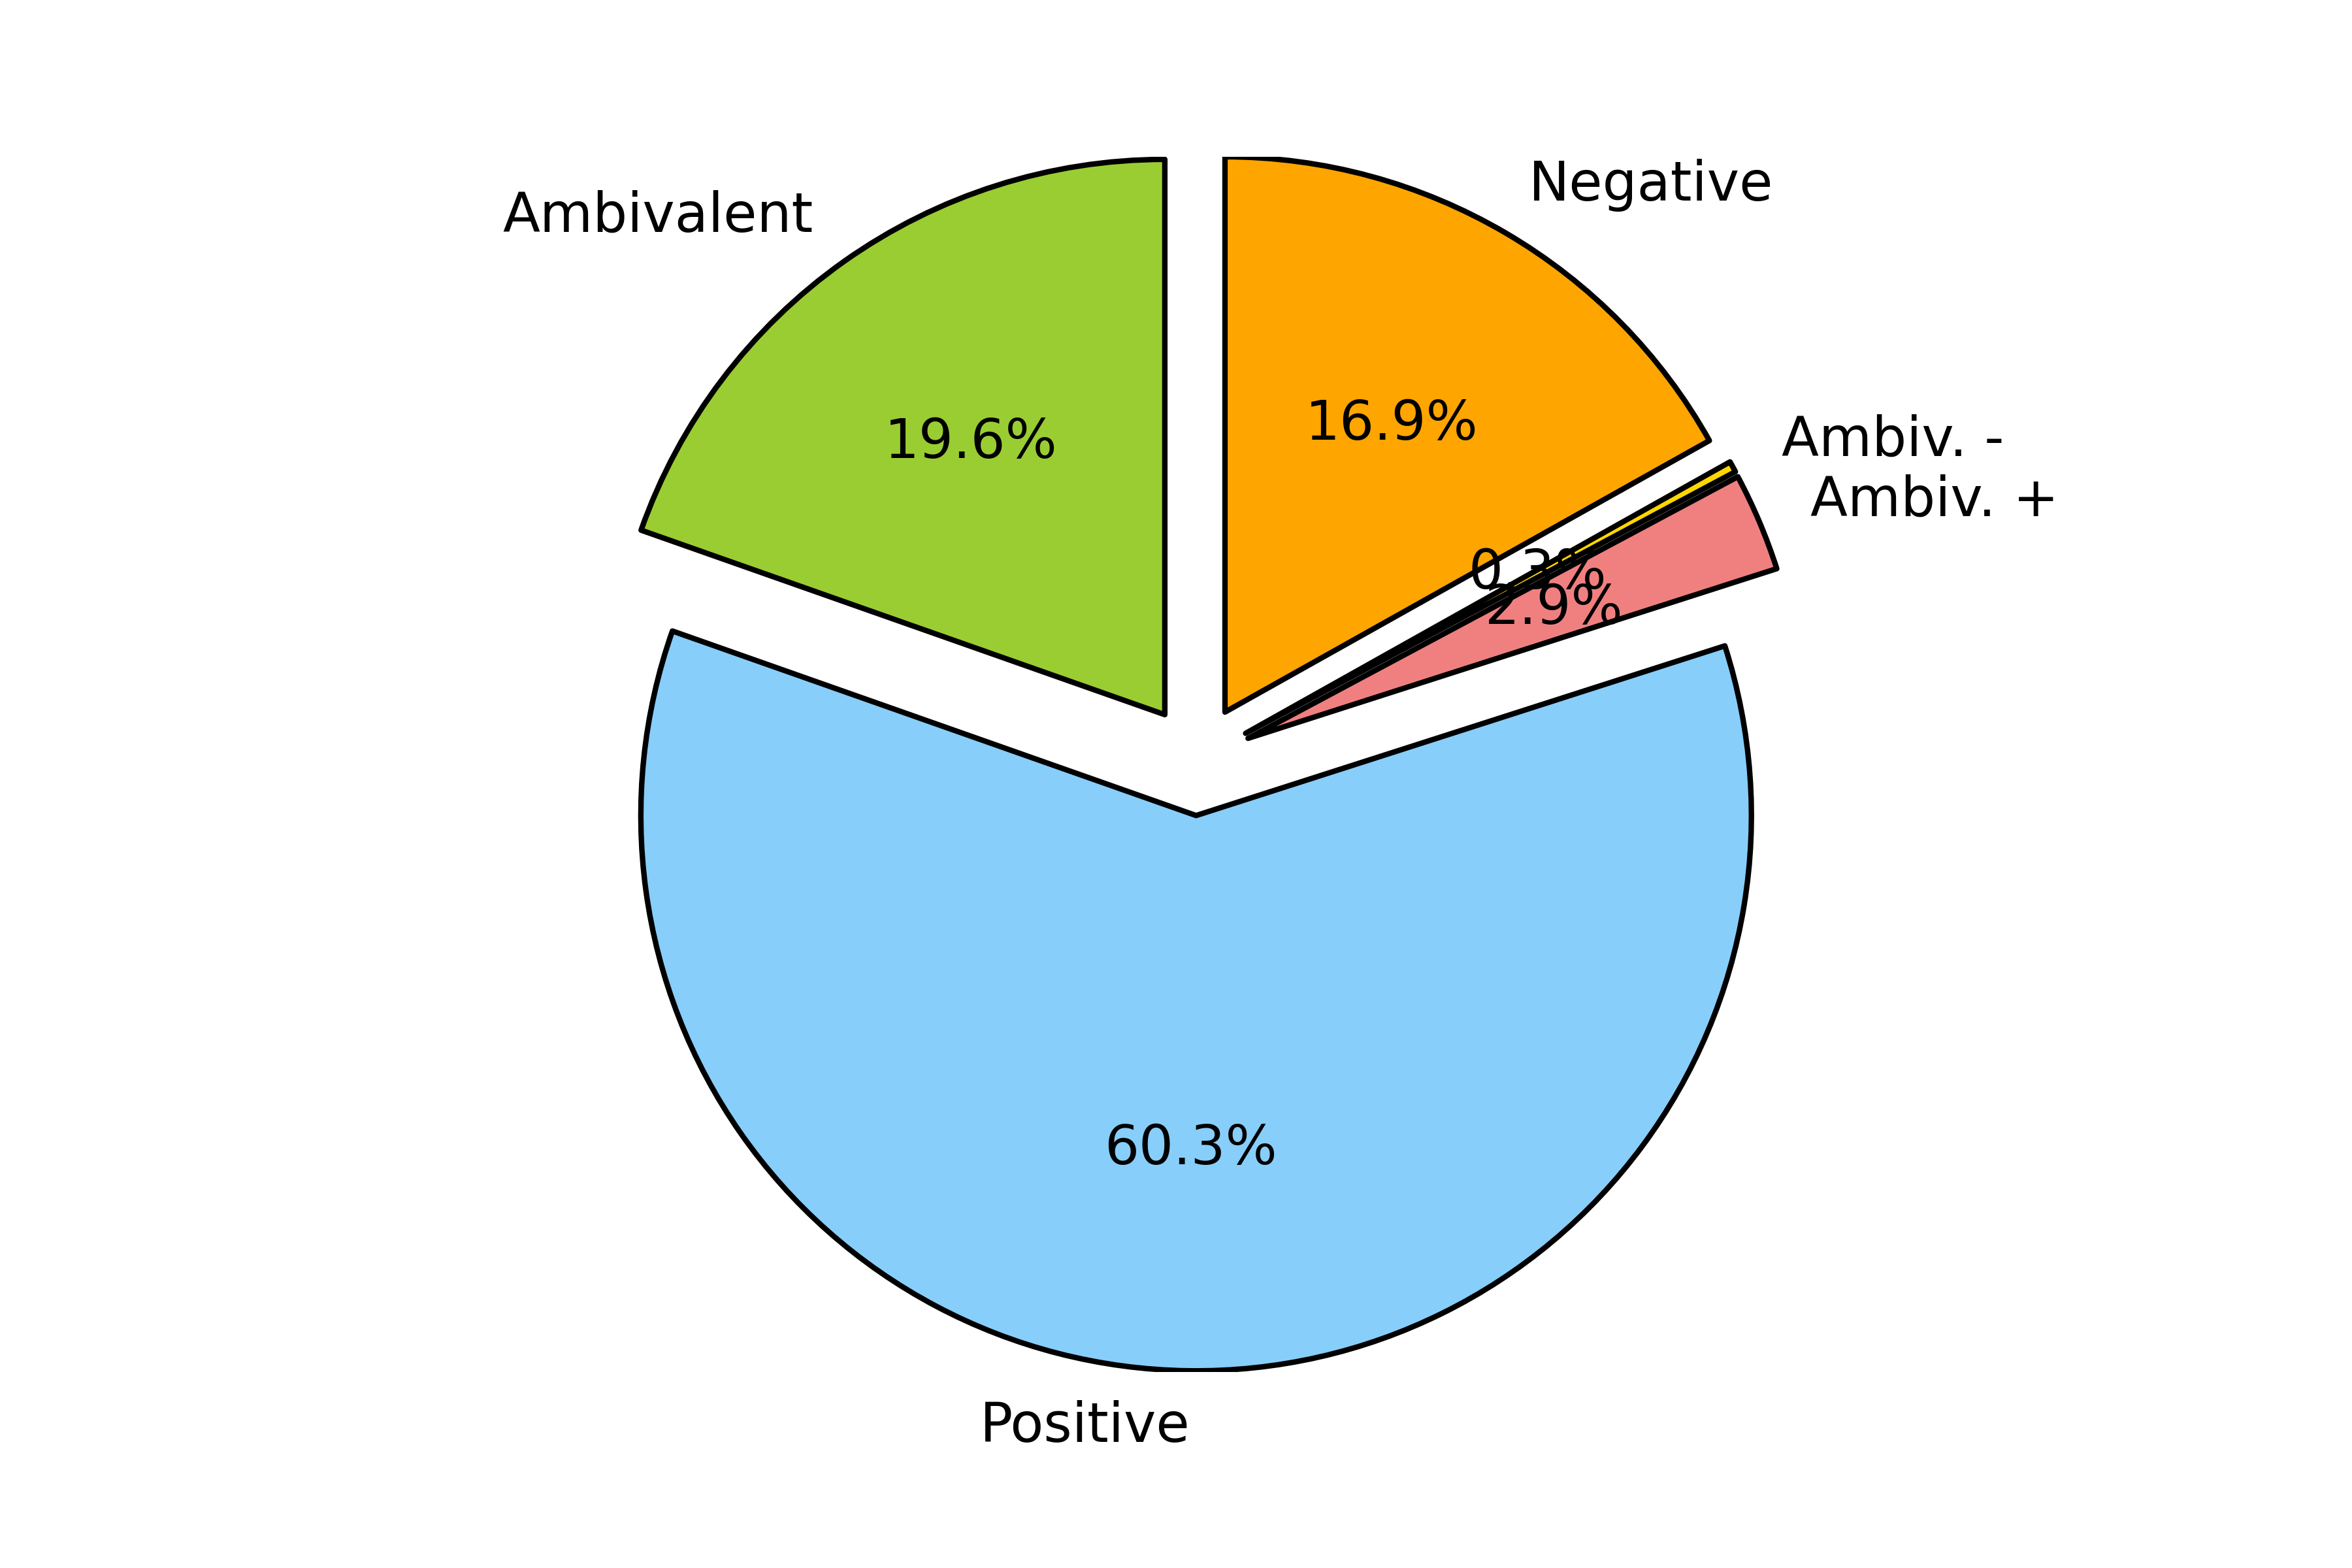
\includegraphics[trim = 1.5cm 0 1.5cm 0, clip = true, width=\textwidth]{../result/charts/emotion_identification_all}
		\caption{总体}
	\end{subfigure}
	\begin{subfigure}[b]{0.45\linewidth}
		\centering
		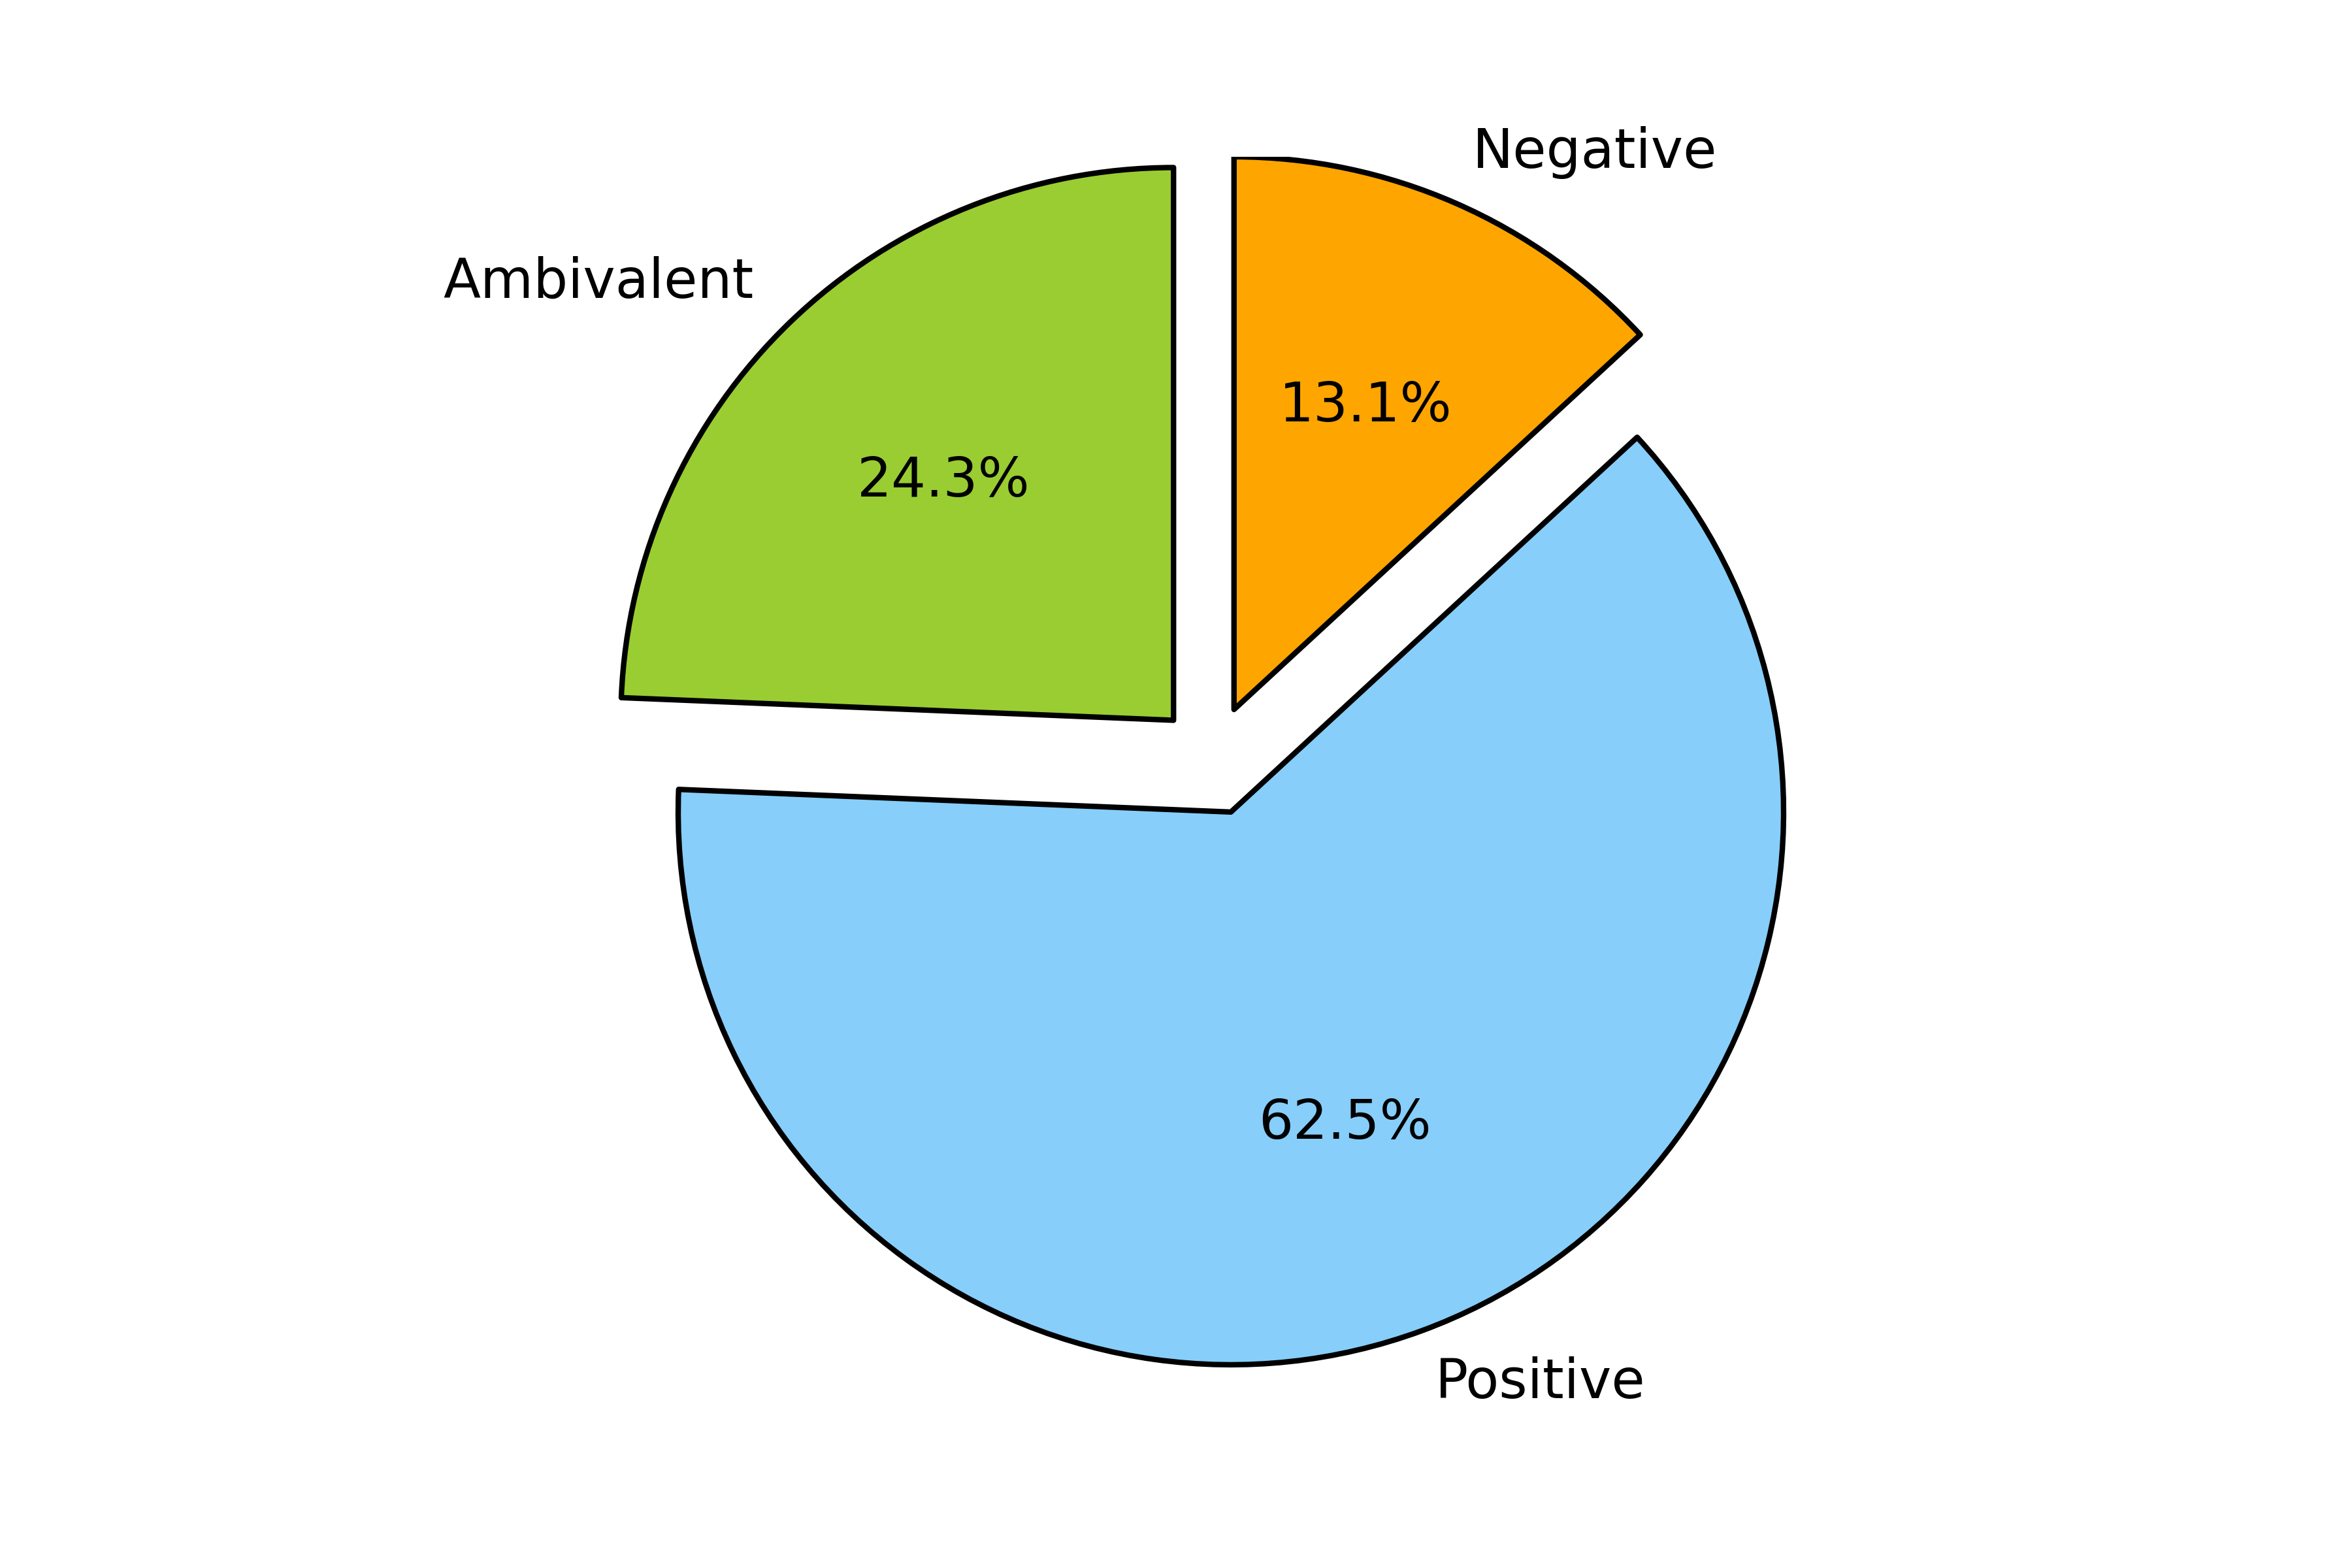
\includegraphics[trim = 1.5cm 0 1.5cm 0, clip = true, width=\textwidth]{../result/charts/emotion_forward}
		\caption{被转发过的微博}
	\end{subfigure}
	\caption{被转发过的微博的情绪分布。}
	\label{fig:emotion_forward}
\end{figure}


\subsection{微博情绪-波浪线}

根据经验,人们在发布积极情绪的微博时,更容易加上波浪线(\~{}),比如“么么哒\~{}\~{}”、“好漂亮\~{}\~{}”等。为了检验这一经验是否符合实际情况,我们对此进行了统计。如图\ref{fig:emotion_tilde}所示,数据显示,含有波浪线的微博积极情占比从60.3\%提高到了65.6\%,而消极情绪的占比降低了6.4\%,符合我们日常经验。

\begin{figure}
	\centering
	\begin{subfigure}[b]{0.45\linewidth}
		\centering
		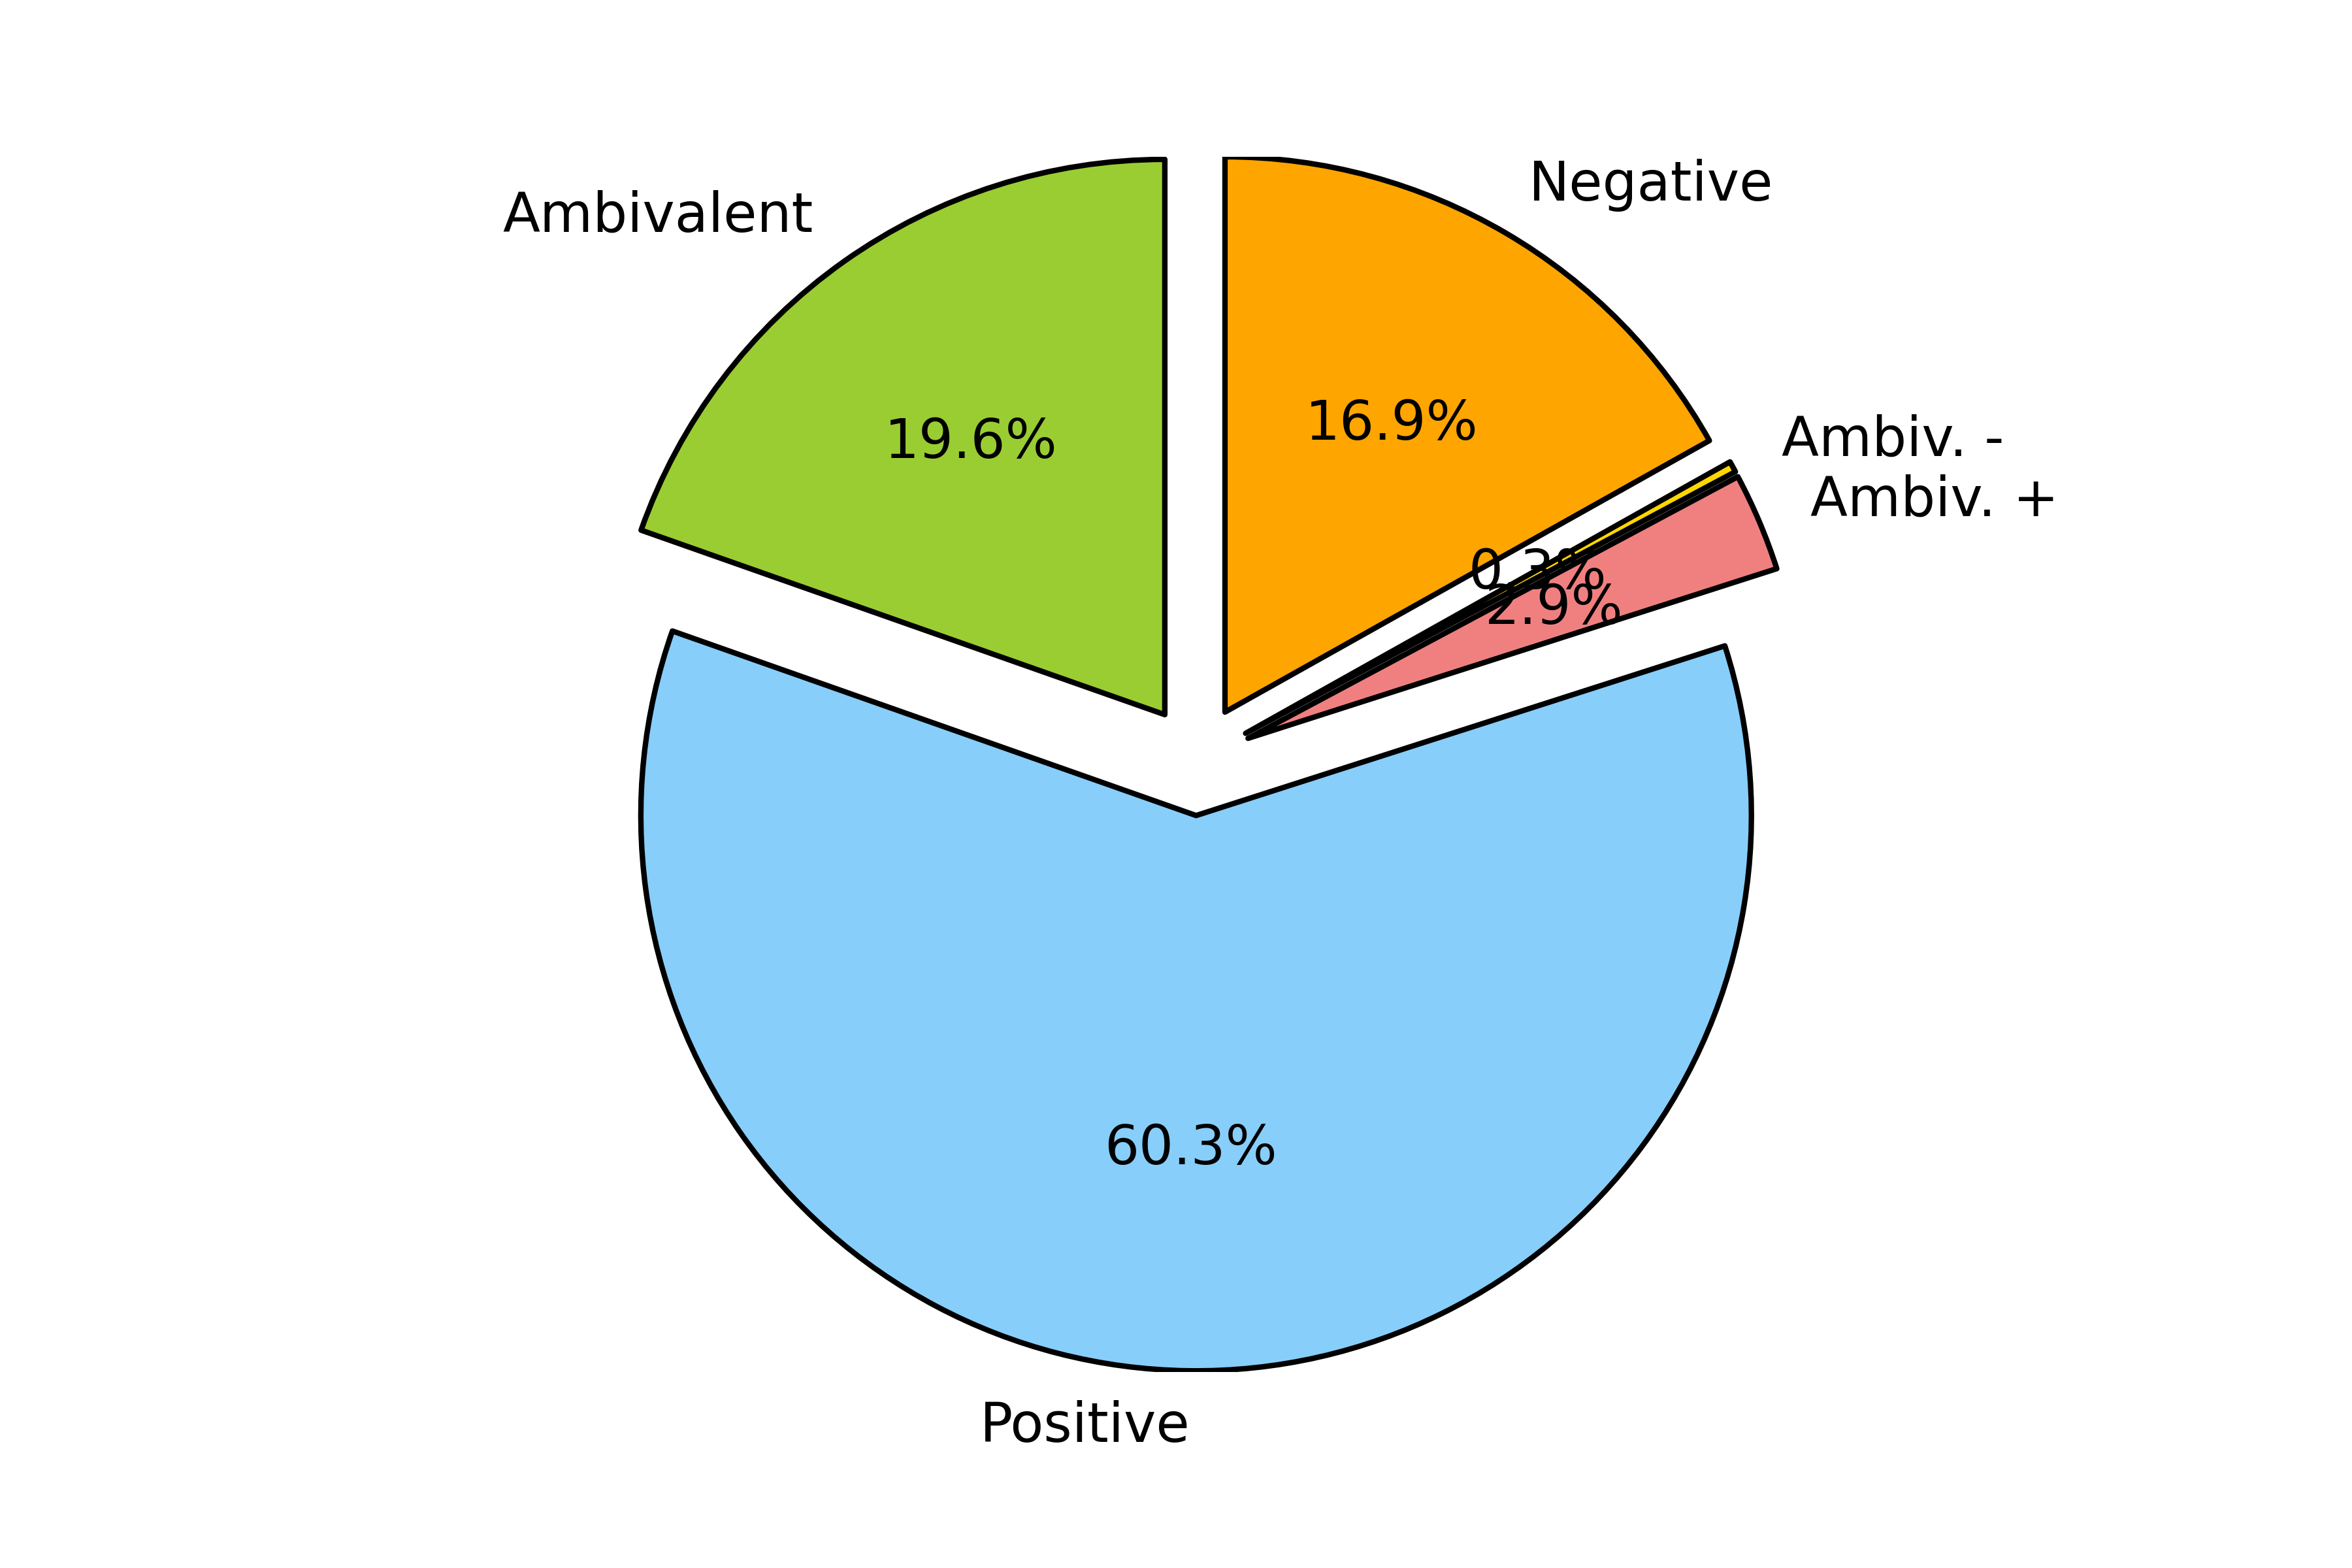
\includegraphics[trim = 1.5cm 0 1.5cm 0, clip = true, width=\textwidth]{../result/charts/emotion_identification_all}
		\caption{总体}
	\end{subfigure}
	\begin{subfigure}[b]{0.45\linewidth}
		\centering
		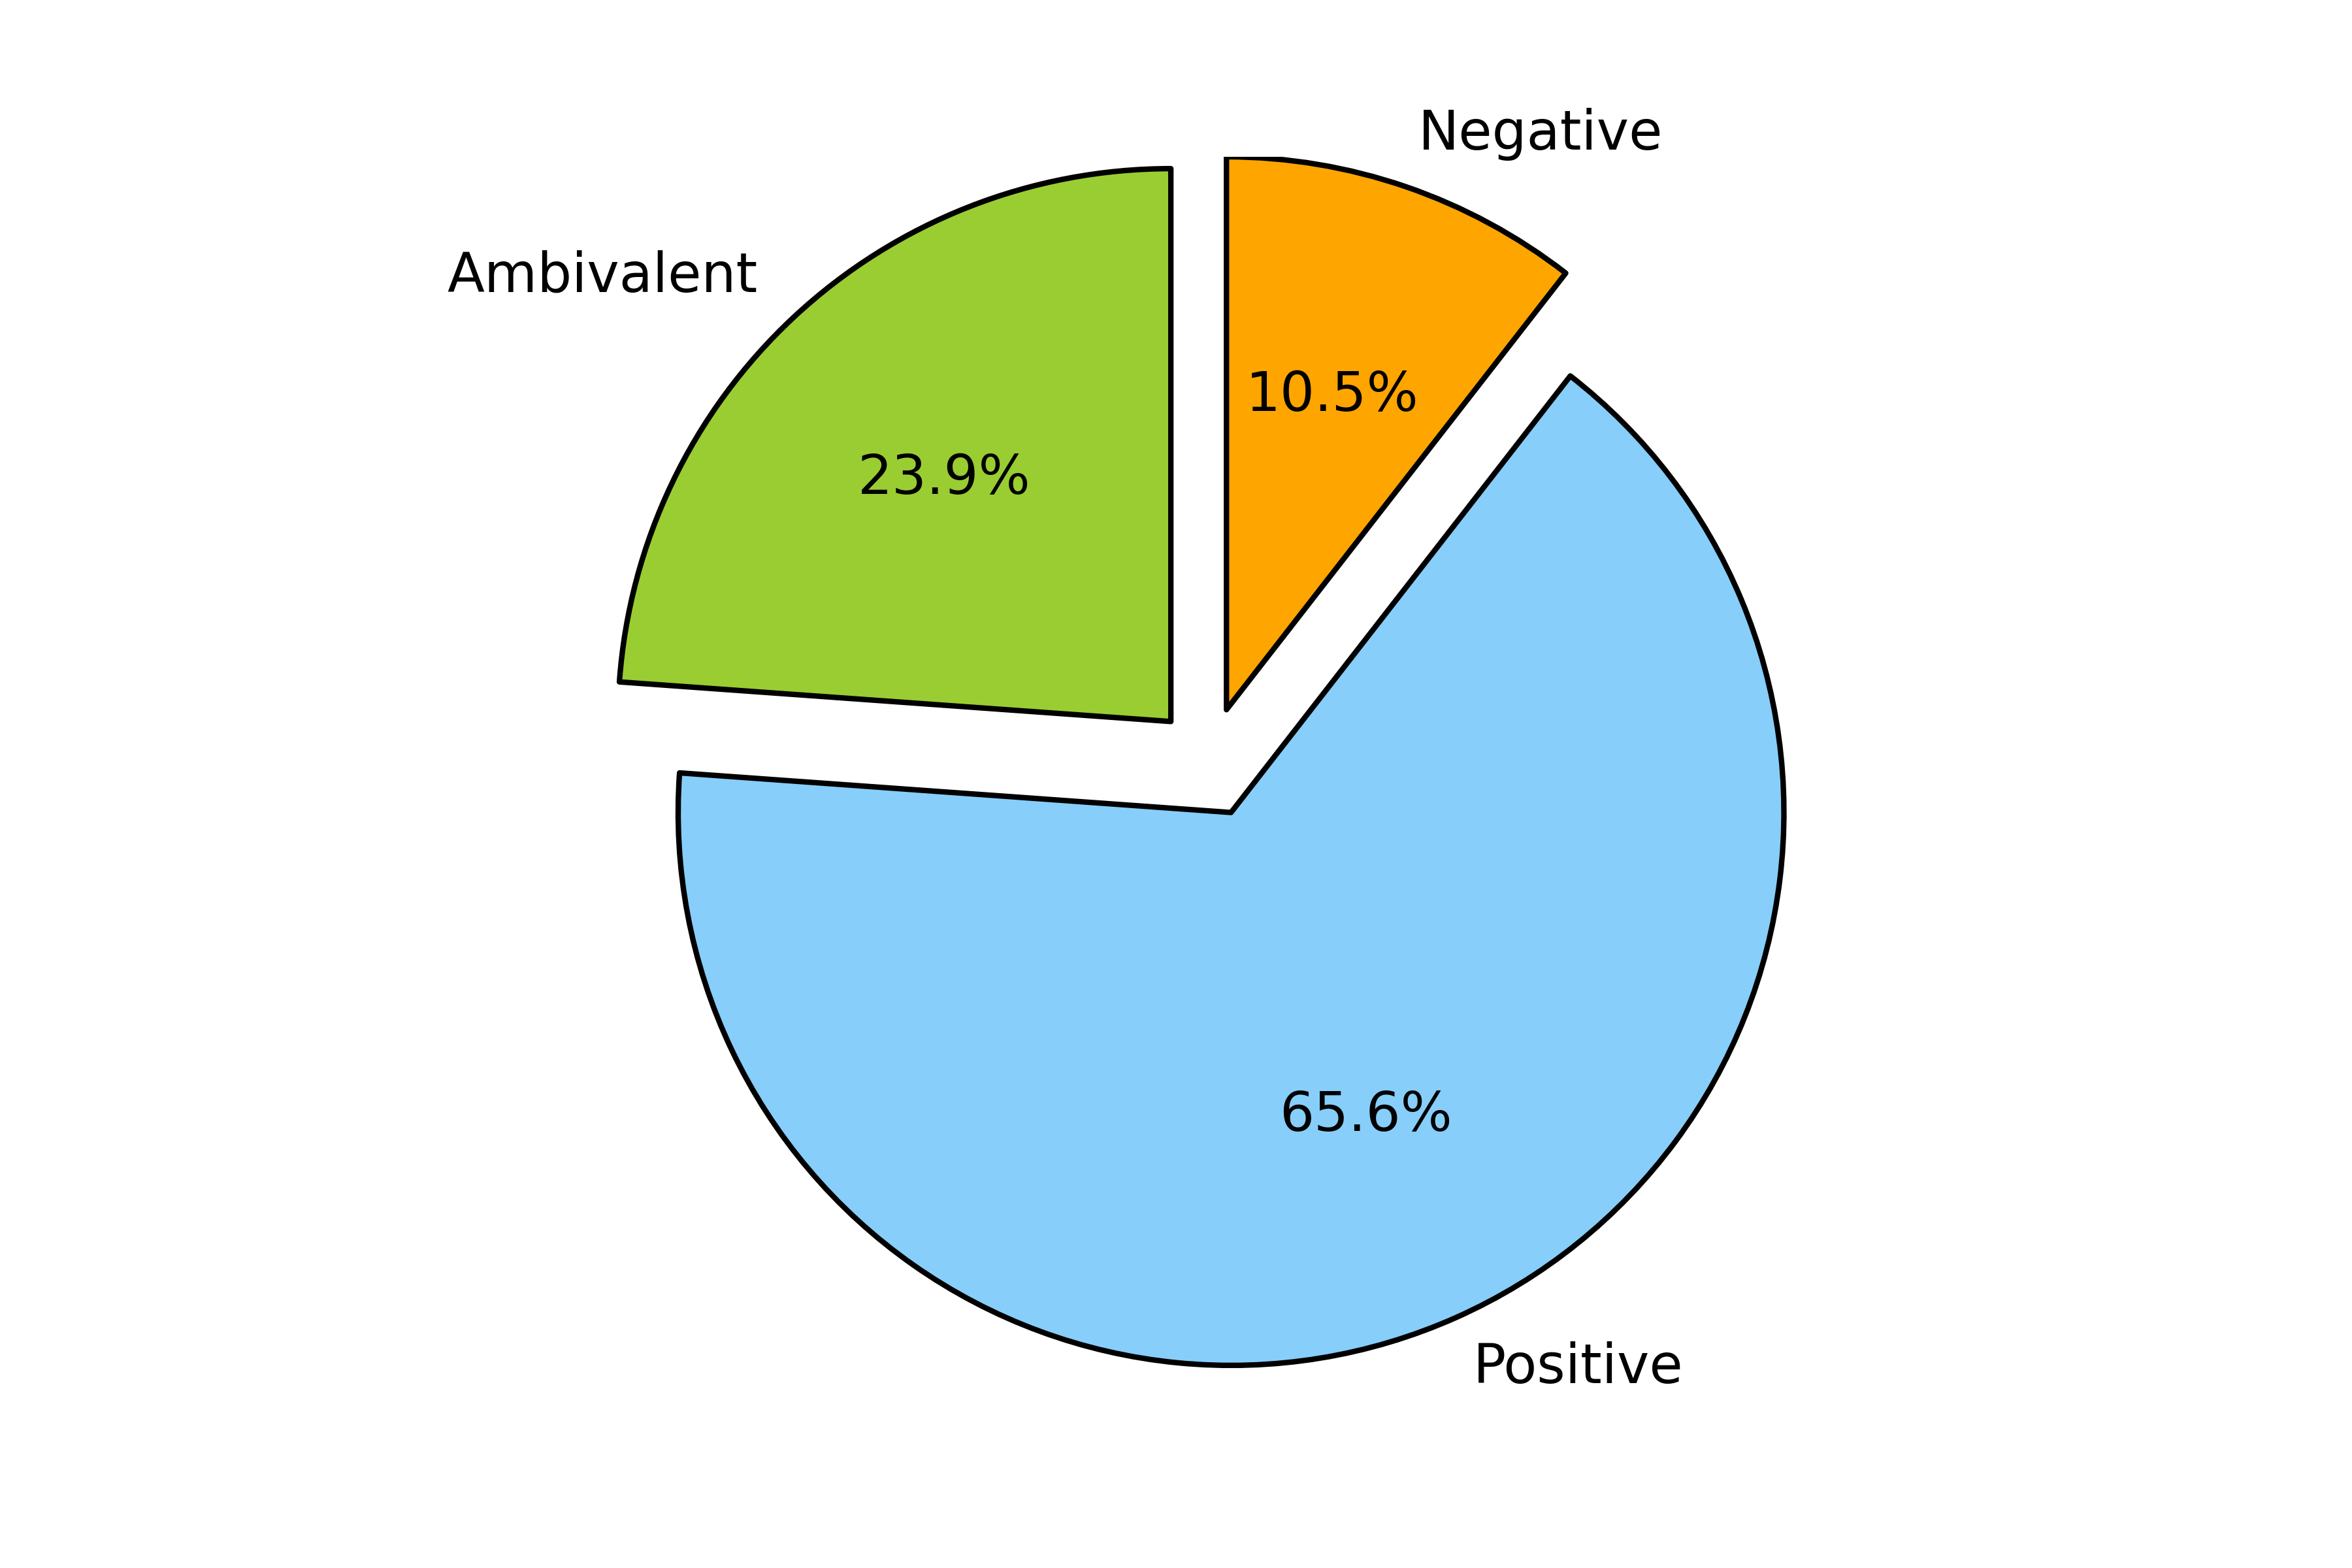
\includegraphics[trim = 1.5cm 0 1.5cm 0, clip = true, width=\textwidth]{../result/charts/emotion_tilde}
		\caption{含有波浪线的微博}
	\end{subfigure}
	\caption{含有波浪线的微博情绪分布情况。}
	\label{fig:emotion_tilde}
\end{figure}

\subsection{微博情绪词典}
\label{subsec:polar_dict}
我们可以首先利用表情和表情畸形词典统计得到的每条微博的情绪,来生成一个描述单词的极性词典,具体做法如下:首先进行分词,这里使用了结巴开源库;之后计算每个词出现的次数和出现在积极微博中的次数,将两者相除,就可以得到一个 $[0, 1]$ 之间的值来衡量这个词的极性。
$$\text{词{\it word}的积极程度}= \frac{\text{{\it word}出现在积极微博中的次数}}{\text{{\it word}出现在所有微博中的次数}}$$
在这里,我们定义如果一个词的积极程度大于0.6,那么就认为其是积极的,介于0.6和0.4之间的是无明显情绪的,小于0.4的是消极的。
表\ref{tbl:polar_dict}列出了最后得到的一些结果,详细的结果保存在/result/emotion_dict.txt。

\begin{table}[]
\centering
\begin{tabular}{|c|c|c|c|c|c|}
\hline
\multicolumn{2}{|c|}{积极} & \multicolumn{2}{c|}{消极} & \multicolumn{2}{c|}{中性} \\ \hline
词           & 积极度        & 词          & 积极度        & 词          & 积极度        \\ \hline
新婚          & 0.87       & 他妈的        & 0.20       & 楼盘         & 0.50       \\ \hline
爱           & 0.89       & 艹          & 0.24       & 毕业生        & 0.50       \\ \hline
天天开心        & 0.89       & 骗          & 0.39       & 高管         & 0.48       \\ \hline
非常感谢        & 0.86       & MLGB       & 0.34       & 美国         & 0.53       \\ \hline
好样          & 0.85       & 睡眠不足       & 0.29       & 组图         & 0.50       \\ \hline
情人节         & 0.71       & 哭泣         & 0.34       & 研究所        & 0.58       \\ \hline
\end{tabular}
\caption{生成的微博情绪词典样例。}
\label{tbl:polar_dict}
\end{table}

\subsection{表情的积极程度}
数据集提供的表情仅用三种值来划分它的极性(积极、消极和无情绪),在此,我们进行了一些统计,得到了每个表情的积极程度。具体做法如下:首先对微博进行分词,分词方法同\ref{subsec:polar_dict}一节;之后使用\ref{subsec:polar_dict}一节得到的极性词典,来计算每一条微博的积极程度,用 $[-1, 1]$ 之间的实数来表示;最后,对每个表情计算其积极程度。
使用下式来计算每一条微博的情绪:
$$\text{微博的情绪} = \frac{\sum{\text{所有出现过的单词的积极程度}}}{\text{\#所有出现过的单词}}$$
使用下式来计算每个表情的积极程度:
$$\text{表情的积极程度} = \frac{\sum{\text{包含该单词的微博的情绪}}}{\text{\#包含该单词的微博}}$$

表\ref{tbl:weighted_expreesions}展示了一部分结果。图\ref{fig:weighted_expressions_top5}是最积极和最消极的表情。

\begin{figure}
	\centering
	
\includegraphics[width=0.35\linewidth]{../result/charts/weighted_expressions_top5}
	\caption{积极程度最高和最低的5个表情,第一行为最积极的表情,第二行为最消极的表情,从左至右程度依次递减。}
	\label{fig:weighted_expressions_top5}
\end{figure}

\begin{table}[]
\centering
\begin{tabular}{|c|c|c|c|}
\hline
\multicolumn{2}{|c|}{积极} & \multicolumn{2}{c|}{消极} \\ \hline
表情            & 积极程度     & 表情          & 积极程度      \\ \hline
{[}太开心{]}     & 0.887    & {[}白眼{]}    & -0.769    \\ \hline
{[}圣诞袜{]}     & 0.905    & {[}哼{]}     & -0.748    \\ \hline
{[}给力{]}      & 0.924    & {[}怒{]}     & -0.855    \\ \hline
{[}来{]}       & 0.853    & {[}悲伤{]}    & -0.785    \\ \hline
{[}礼物{]}      & 0.879    & {[}鄙视{]}    & -0.782    \\ \hline
{[}可爱{]}      & 0.898    & {[}委屈{]}    & -0.710    \\ \hline
\end{tabular}
\caption{表情的积极程度样例}
\label{tbl:weighted_expreesions}
\end{table}

\subsection{性能对比}
性能对比分为两部分,分别针对单机与分布环境下的效率,以及分布式环境下大小数据之间的关系。

第一部分我们使用分词预处理的程序作为测试对象。测试时,首先将分词程序部署到集群上,分配6个执行器( executor )运行;之后直接在集群的其中的一台机子上运行相同的程序 (仅1个执行器)。结果显示,运行在分布式环境上的程序耗时 {\it 21m31s},而运行在单机上的程序耗时 {\it 1h48m19s}。可以看到,分布式环境上的程序性能有明显的提升。但是,值得注意的是,在分布式环境下使用了6个执行器的程序并没有达到6倍的性能提升,这可能是由于网络延迟、任务调度和数据管理消耗了一些额外资源造成的。为了研究分布式程序额外资源的消耗,我们进行了第二部分的对比。

第二部分的对比我们使用计算表情积极程度的程序作为测试对象。两次测试均使用相同的配置部署,不同的是使用的数据集大小。第一个程序输入小的数据集,大小为原始数据集的 $\frac{1}{20}$ ,第二个程序输入原始大小的数据集。第一个程序耗时 {\it 3m46s},第二个程序耗时 {\it 53m22s}。第二个程序要比第一个程序运行时间的20倍来得少,这种关系说明有一些调度管理的任务所消耗的时间要比数据集的增长来的缓慢。

\newpage
\renewcommand\refname{参考文献}
\bibliographystyle{plain}
\bibliography{Report}

\end{CJK}
\end{spacing}
\end{document}
